\documentclass[handout,code={Graphs I},title={Introduction, DFS, BFS}]{../share/cpslide}
\usetikzlibrary{arrows.meta}
\usepackage{subcaption}
\usepackage{adjustbox}
\slideinit

\begin{document}

\slidebegin



\newcommand{\graph}[2]{\begin{tikzpicture}
    \node[shape=circle,draw=black, ultra thick] (A) at (0,0) {A};
    \node[shape=circle,draw=black, ultra thick] (B) at (0,#1*1.5) {B};
    \node[shape=circle,draw=black, ultra thick] (C) at (#1*1.25 ,#1*2) {C};
    \node[shape=circle,draw=black, ultra thick] (D) at (#1*1.25,#1*0.5) {D};
    \node[shape=circle,draw=black, ultra thick] (E) at (#1*2.5, -#1*0.5) {E};
    \node[shape=circle,draw=black, ultra thick] (F) at (#1*2.5,#1*1.5) {F} ;

    \path [#2,very thick](A) edge  (B);
    \path [#2,very thick](B) edge  (C);
    \path [#2,very thick](A) edge (D);
    \path [#2,very thick](D) edge  (C);
    \path [#2,very thick](A) edge  (E);
    \path [#2,very thick](D) edge  (E);
    \path [#2,very thick](D) edge  (F);
    \path [#2,very thick](C) edge  (F);
    \path [#2,very thick](E) edge (F);
   

\end{tikzpicture}
}

\newcommand{\directedgraph}[2]{\graph{#1}{->}}
\newcommand{\undirectedgraph}[2]{\graph{#1}{-}}

\newcommand{\wgraph}[2]{\begin{tikzpicture}
    \node[shape=circle,draw=black, ultra thick] (A) at (0,0) {A};
    \node[shape=circle,draw=black, ultra thick] (B) at (0,#1*1.5) {B};
    \node[shape=circle,draw=black, ultra thick] (C) at (#1*1.25 ,#1*2) {C};
    \node[shape=circle,draw=black, ultra thick] (D) at (#1*1.25,#1*0.5) {D};
    \node[shape=circle,draw=black, ultra thick] (E) at (#1*2.5, -#1*0.5) {E};
    \node[shape=circle,draw=black, ultra thick] (F) at (#1*2.5,#1*1.5) {F} ;

\begin{scope}[>={Stealth[black]},
              every node/.style={fill=white,rectangle, scale=0.7}]
    \path [#2,very thick](A) edge node{$3$} (B);
    \path [#2,very thick](B) edge node{$5$} (C);
    \path [#2,very thick](A) edge node{$9$} (D);
    \path [#2,very thick](D) edge node{$2$} (C);
    \path [#2,very thick](A) edge node{$1$} (E);
    \path [#2,very thick](D) edge node{$4$} (E);
    \path [#2,very thick](D) edge node{$3$} (F);
    \path [#2,very thick](C) edge node{$6$} (F);
    \path [#2,very thick](E) edge node{$7$} (F);

\end{scope} 

\end{tikzpicture}
}

\newcommand{\directedwgraph}[2]{\wgraph{#1}{->}}
\newcommand{\undirectedwgraph}[2]{\wgraph{#1}{-}}

\section{What is a graph ?}

\begin{frame}{What is a graph ?}

A graph can be described as a set of points linked or not together. \\

The points are called \textbf{Vertices} and the links \textbf{Edges}. \\  

For example, a graph can represent a country : the cities are the vertices and the road are the edges. 


\end{frame}

\begin{frame}{Graph : example}
\begin{figure}
\center
\undirectedgraph{1}
\\
\\
An example of graph
\end{figure}

\begin{itemize}
\item 6 Vertices : A,B,C,D,E and F 
\item 9 Edges : (A,B), (B,C), (A,D), (D,C), (A,E), (D,E), (D,F), (C,F) and (E,F)
\end{itemize}
\end{frame}



\begin{frame}{Terminology and definitions}
A graph can be said to be :
\begin{itemize}
\item \textbf{Undirected} if all edges are both-way
\item \textbf{Directed} if there are one-way edges
\item \textbf{Weighted} if there is a number associated with each edge (like a distance)
\item \textbf{Unweighted} otherwise
\item \textbf{Connected} if there is a path between all pair of vertices
\item \textbf{Acyclic} if there is no loop
\item \textbf{Dense} if there is an edge between all pair of vertices
\end{itemize}

\begin{warning}
There may be more than one edge between two vertices. The graph is then called a Multigraph (otherwise it's a simple graph). 
\end{warning}

\end{frame}


\begin{frame}{Terminology and definitions}
Two main numbers in a graph

\begin{itemize}
\item $V$ the vertices number
\item $E$ the edges number
\end{itemize}
The degree of a vertex is the number of edges linking to this vertex.

\begin{figure}
\center
\begin{adjustbox}{max totalsize={.6\textwidth}{.6\textheight}}
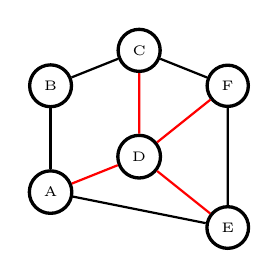
\begin{tikzpicture}[scale=0.6]
    \node[shape=circle,draw=black, very thick] (A) at (0,0) {\tiny{A}};
    \node[shape=circle,draw=black, very thick] (B) at (0,1.5*1.5) {\tiny{B}};
    \node[shape=circle,draw=black, very thick] (C) at (1.5*1.25 ,1.5*2) {\tiny{C}};
    \node[shape=circle,draw=black, very thick] (D) at (1.5*1.25,1.5*0.5) {\tiny{D}};
    \node[shape=circle,draw=black, very thick] (E) at (1.5*2.5, -1.5*0.5) {\tiny{E}};
    \node[shape=circle,draw=black, very thick] (F) at (1.5*2.5,1.5*1.5) {\tiny{F}} ;

    \path [-, thick](A) edge  (B);
    \path [-, thick](B) edge  (C);
    \path [-, thick, red](A) edge (D);
    \path [-, thick, red](D) edge  (C);
    \path [-, thick](A) edge  (E);
    \path [-, thick, red](D) edge  (E);
    \path [-, thick, red](D) edge  (F);
    \path [-, thick](C) edge  (F);
    \path [-, thick](E) edge (F);
   

\end{tikzpicture}
\end{adjustbox}
\\
$deg(D) = 4$
\end{figure}


\end{frame}





\begin{frame}{Tree}
A simple undirected graph is called a \textbf{Tree} if there is exactly one path between all pair of vertices. A tree is always acyclic. Being a tree and having $E = V-1$ are equivalent (except if there are multiple vertices between two nodes).
\end{frame}

\begin{frame}{Directed graph : example}
\begin{figure}
\center
\directedgraph{1.5}
\\
\\
An example of directed graph
\end{figure}
\end{frame}

\begin{frame}{Weighted graph : example}
\begin{figure}
\center
\undirectedwgraph{1.5}
\\
\\
An example of weighted graph
\end{figure}

\end{frame}

\begin{frame}{Tree : example}
\begin{figure}
\center 
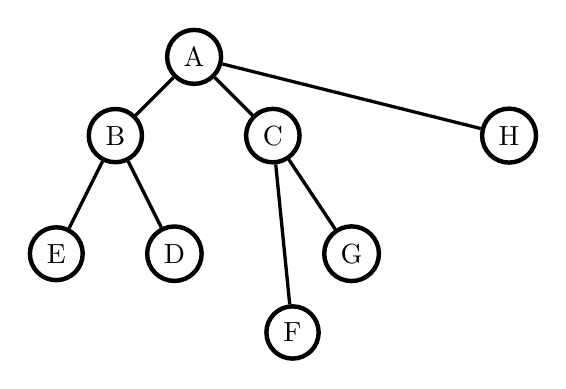
\begin{tikzpicture}
    \node[shape=circle,draw=black, ultra thick] (A) at (0,0) {A};
    \node[shape=circle,draw=black, ultra thick] (B) at (-1, -1) {B};
    \node[shape=circle,draw=black, ultra thick] (C) at (1, -1) {C};
    \node[shape=circle,draw=black, ultra thick] (D) at (-0.25, -2.5) {D};
    \node[shape=circle,draw=black, ultra thick] (E) at (-1.75, -2.5) {E};
    \node[shape=circle,draw=black, ultra thick] (F) at (1.25, -3.5) {F} ;
    \node[shape=circle,draw=black, ultra thick] (G) at (2, -2.5) {G} ;
    \node[shape=circle,draw=black, ultra thick] (H) at (4, -1) {H} ;

    \path [-,very thick](A) edge  (B);
    \path [-,very thick](A) edge  (C);
    \path [-,very thick](A) edge  (H);
    \path [-,very thick](B) edge  (D);
    \path [-,very thick](B) edge  (E);
    \path [-,very thick](C) edge  (F);
    \path [-,very thick](C) edge  (G);

   

\end{tikzpicture}
\\
An example of a tree
\end{figure}
\end{frame}

\begin{frame}{Connected vs Unconnected}
\begin{figure}
\center
\begin{subfigure}[b, scale=0.8]{0.4\textwidth}
\center
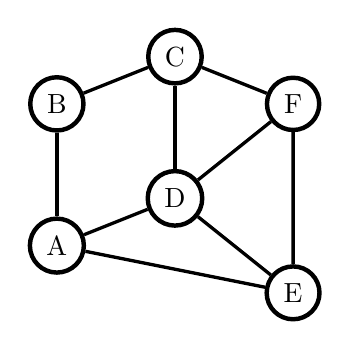
\begin{tikzpicture}[scale=0.8]
    \node[shape=circle,draw=black, ultra thick] (A) at (0,0) {A};
    \node[shape=circle,draw=black, ultra thick] (B) at (0,1.5*1.5) {B};
    \node[shape=circle,draw=black, ultra thick] (C) at (1.5*1.25 ,1.5*2) {C};
    \node[shape=circle,draw=black, ultra thick] (D) at (1.5*1.25,1.5*0.5) {D};
    \node[shape=circle,draw=black, ultra thick] (E) at (1.5*2.5, -1.5*0.5) {E};
    \node[shape=circle,draw=black, ultra thick] (F) at (1.5*2.5,1.5*1.5) {F} ;

    \path [-,very thick](A) edge  (B);
    \path [-,very thick](B) edge  (C);
    \path [-,very thick](A) edge (D);
    \path [-,very thick](D) edge  (C);
    \path [-,very thick](A) edge  (E);
    \path [-,very thick](D) edge  (E);
    \path [-,very thick](D) edge  (F);
    \path [-,very thick](C) edge  (F);
    \path [-,very thick](E) edge (F);
   

\end{tikzpicture}
\\ 
Connected

\end{subfigure}
\begin{subfigure}[b, scale=0.8]{0.4\textwidth}
\center
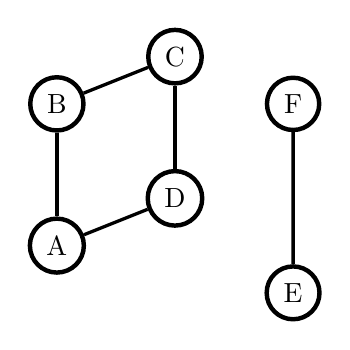
\begin{tikzpicture}[scale=0.8]
    \node[shape=circle,draw=black, ultra thick] (A) at (0,0) {A};
    \node[shape=circle,draw=black, ultra thick] (B) at (0,1.5*1.5) {B};
    \node[shape=circle,draw=black, ultra thick] (C) at (1.5*1.25 ,1.5*2) {C};
    \node[shape=circle,draw=black, ultra thick] (D) at (1.5*1.25,1.5*0.5) {D};
    \node[shape=circle,draw=black, ultra thick] (E) at (1.5*2.5, -1.5*0.5) {E};
    \node[shape=circle,draw=black, ultra thick] (F) at (1.5*2.5,1.5*1.5) {F} ;

    \path [-,very thick](A) edge  (B);
    \path [-,very thick](B) edge  (C);
    \path [-,very thick](A) edge (D);
    \path [-,very thick](D) edge  (C);
    \path [-,very thick](E) edge (F);
   

\end{tikzpicture}
\\ 
Unconnected
\end{subfigure}
\end{figure}

\end{frame}

\section{Graph Representation}

\begin{frame}{Representing a graph}
There are three ways of representing a graph : 
\begin{itemize}
\item In the form of an edges list (we won't use it here)
\item In the form of an adjacency matrix
\item In the form of an adjacency list.

\end{itemize}
\end{frame}

\begin{frame}{Adjacency matrix}
\begin{columns}[T] % align columns
\begin{column}[b]{0.6\linewidth}
\begin{minipage}{\linewidth}

\begin{figure}
\begin{adjustbox}{max totalsize={.4\textwidth}{.4\textheight}}
\undirectedgraph{1.5}
\\
\end{adjustbox}
\end{figure}

\begin{itemize}
\item Store connection in a boolean matrix
\item $a_{ij} =$ true if vertices $i$ and $j$ are connected
\item \O{V^2} memory 
\end{itemize}
\end{minipage}
\end{column}
\begin{column}[b]{0.4\linewidth}
\begin{minipage}{\linewidth}


$$
\begin{pmatrix}
0 & 1 & 0 & 1 & 1 & 0\\ 
1 & 0 & 1 & 0 & 0 & 0\\
0 & 1 & 0 & 1 & 0 & 1\\
1 & 0 & 1 & 0 & 1 & 1\\
1 & 0 & 0 & 1 & 0 & 1\\
0 & 0 & 1 & 1 & 1 & 0\\

\end{pmatrix}
$$\\
As the graph is undirected, the matrix is symmetric.
\end{minipage}
\end{column}
\end{columns}

\end{frame}

\begin{frame}{Adjacency matrix for directed graph}
\begin{columns}[T] % align columns
\begin{column}[b]{0.6\linewidth}
\begin{minipage}{\linewidth}

\begin{figure}
\begin{adjustbox}{max totalsize={.4\textwidth}{.4\textheight}}
\directedgraph{1.5}
\\
\end{adjustbox}
\end{figure}

\begin{itemize}
\item $a_{ij} =$ true if there is an edge from $i$ to $j$
\item $a_{ij} \neq a_{ji}$ in most cases
\end{itemize}
\end{minipage}
\end{column}
\begin{column}[b]{0.4\linewidth}
\begin{minipage}{\linewidth}


$$
\begin{pmatrix}
0 & 1 & 0 & 1 & 1 & 0\\ 
0 & 0 & 1 & 0 & 0 & 0\\
0 & 0 & 0 & 0 & 0 & 1\\
0 & 0 & 1 & 0 & 1 & 1\\
0 & 0 & 0 & 0 & 0 & 1\\
0 & 0 & 0 & 0 & 0 & 0\\

\end{pmatrix}
$$\\
Not symmetric

\end{minipage}
\end{column}
\end{columns}

\end{frame}

\begin{frame}{Adjacency matrix for weighted graph}
\begin{columns}[T] % align columns
\begin{column}[b]{0.6\linewidth}
\begin{minipage}{\linewidth}

\begin{figure}
\begin{adjustbox}{max totalsize={.4\textwidth}{.4\textheight}}
\undirectedwgraph{1.5}
\\
\end{adjustbox}
\end{figure}

\begin{itemize}
\item Replace the boolean array by an integer (or double) array
\item $a_{ij}= $ distance (or weight) from $i$ to $j$
\item $a_{ij}$ symmetric if the graph is not directed
\end{itemize}
\end{minipage}
\end{column}
\begin{column}[b]{0.4\linewidth}
\begin{minipage}{\linewidth}


$$
\begin{pmatrix}
0 & 3 & 0 & 9 & 1 & 0\\ 
3 & 0 & 5 & 0 & 0 & 0\\
0 & 5 & 0 & 2 & 0 & 6\\
9 & 0 & 2 & 0 & 3 & 4\\
1 & 0 & 0 & 3 & 0 & 7\\
0 & 0 & 6 & 4 & 7 & 0\\

\end{pmatrix}
$$\\

You can't use a adjacency matrix on a Multigraph !.


\end{minipage}
\end{column}
\end{columns}

\end{frame}

\begin{frame}{Adjacency list}
\begin{columns}[T] % align columns
\begin{column}[b]{0.6\linewidth}
\begin{minipage}{\linewidth}

\begin{figure}
\begin{adjustbox}{max totalsize={.4\textwidth}{.4\textheight}}
\undirectedgraph{1.5}
\\
\end{adjustbox}
\end{figure}

\begin{itemize}
\item Store connection in array of lists
\item \ci{adj[i]} is a list containing the adjacency vertices of vertex $i$
\item Only way to work in a Multigraph.
\item \O{E} memory 
\end{itemize}
\end{minipage}
\end{column}
\begin{column}[b]{0.4\linewidth}
\begin{minipage}{\linewidth}
$A: \{B, D, E\}$\\
$B: \{A, C\}$\\
$C: \{B, D, F\}$\\
$D: \{A, C, E, F\}$\\
$E: \{A, D, F\}$\\
$F: \{C, D, E\}$\\

If the graph is undirected, don't forget to add the edges in both ways !


\end{minipage}
\end{column}
\end{columns}


\end{frame}

\begin{frame}{Adjacency list for weighted graph}
\begin{columns}[T] % align columns
\begin{column}[b]{0.6\linewidth}
\begin{minipage}{\linewidth}

\begin{figure}
\begin{adjustbox}{max totalsize={.4\textwidth}{.4\textheight}}
\undirectedwgraph{1.5}
\\
\end{adjustbox}
\end{figure}

\begin{itemize}
\item Same principle 
\item For each connexion, store a pair of number : the destination vertex and the edge weight.
\item Use an array of \ci{vector<pair<int, int\textgreater{}\textgreater}

\end{itemize}
\end{minipage}
\end{column}
\begin{column}[b]{0.45\linewidth}
\begin{minipage}{\linewidth}
\footnotesize{
$A: \{(B, 3), (D, 9), (E, 1)\}$\\
$B: \{(A, 3), (C, 5)\}$\\
$C: \{(B, 5), (D, 2), (F, 6)\}$\\
$D: \{(A, 9), (C, 2), (E, 4), (F, 3)\}$\\
$E: \{(A, 1), (D,4), (F, 7)\}$\\
$F: \{(C, 6), (D,3) , (E, 7)\}$\\
}



\end{minipage}
\end{column}
\end{columns}


\end{frame}

\begin{frame}{Tree parent representation}
\begin{itemize}
\item Chose a vertex called the \textbf{root}
\item Each vertex will have a parent except for the root
\item Build it recursively
\end{itemize}
\begin{columns}
\begin{column}[b]{0.6\linewidth}

\begin{minipage}{\linewidth}

\begin{figure}
\center
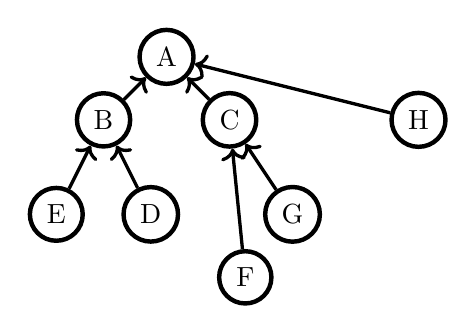
\begin{tikzpicture}[scale=0.8]
    \node[shape=circle,draw=black, ultra thick] (A) at (0,0) {A};
    \node[shape=circle,draw=black, ultra thick] (B) at (-1, -1) {B};
    \node[shape=circle,draw=black, ultra thick] (C) at (1, -1) {C};
    \node[shape=circle,draw=black, ultra thick] (D) at (-0.25, -2.5) {D};
    \node[shape=circle,draw=black, ultra thick] (E) at (-1.75, -2.5) {E};
    \node[shape=circle,draw=black, ultra thick] (F) at (1.25, -3.5) {F} ;
    \node[shape=circle,draw=black, ultra thick] (G) at (2, -2.5) {G} ;
    \node[shape=circle,draw=black, ultra thick] (H) at (4, -1) {H} ;

    \path [<-,very thick](A) edge  (B);
    \path [<-,very thick](A) edge  (C);
    \path [<-,very thick](A) edge  (H);
    \path [<-,very thick](B) edge  (D);
    \path [<-,very thick](B) edge  (E);
    \path [<-,very thick](C) edge  (F);
    \path [<-,very thick](C) edge  (G);

   

\end{tikzpicture}
\end{figure}
\end{minipage}
\end{column}
\begin{column}[b]{0.4\linewidth}
\begin{minipage}{\linewidth}
\begin{center}
Parents :
\end{center}
\footnotesize{
$A : $ has no parent (root)\\
$B : A$\\
$C : A$\\
$D : B$\\
$E : B$\\
$F : C$\\
$G : C$\\
$H : A$\\
}
\end{minipage}
\end{column}
\end{columns}

\end{frame}

\begin{frame}{Tree list of children representation}
\begin{itemize}
\item Transposed of parents representation
\item If $X$ is parent of $Y$, $Y$ is child of $X$
\item Store the children of a vertex in an array
\item A vertex without child is called a \textbf{leaf}
\end{itemize}
\begin{columns}
\begin{column}[b]{0.6\linewidth}

\begin{minipage}{\linewidth}

\begin{figure}
\center
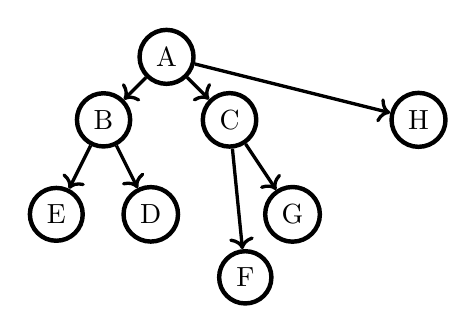
\begin{tikzpicture}[scale=0.8]
    \node[shape=circle,draw=black, ultra thick] (A) at (0,0) {A};
    \node[shape=circle,draw=black, ultra thick] (B) at (-1, -1) {B};
    \node[shape=circle,draw=black, ultra thick] (C) at (1, -1) {C};
    \node[shape=circle,draw=black, ultra thick] (D) at (-0.25, -2.5) {D};
    \node[shape=circle,draw=black, ultra thick] (E) at (-1.75, -2.5) {E};
    \node[shape=circle,draw=black, ultra thick] (F) at (1.25, -3.5) {F} ;
    \node[shape=circle,draw=black, ultra thick] (G) at (2, -2.5) {G} ;
    \node[shape=circle,draw=black, ultra thick] (H) at (4, -1) {H} ;

    \path [->,very thick](A) edge  (B);
    \path [->,very thick](A) edge  (C);
    \path [->,very thick](A) edge  (H);
    \path [->,very thick](B) edge  (D);
    \path [->,very thick](B) edge  (E);
    \path [->,very thick](C) edge  (F);
    \path [->,very thick](C) edge  (G);

   

\end{tikzpicture}
\end{figure}
\end{minipage}
\end{column}
\begin{column}[b]{0.4\linewidth}
\begin{minipage}{\linewidth}
\begin{center}
Children :
\end{center}
\footnotesize{
$A : \{B, C, H\}$\\
$B : \{D, E\}$\\
$C : \{F, G\}$\\
$D : \{\}$ (leaf)\\
$E : \{\}$ (leaf)\\
$F : \{\}$ (leaf)\\
$G : \{\}$ (leaf)\\
$H : \{\}$ (leaf)\\
}
\end{minipage}
\end{column}
\end{columns}

\end{frame}

\begin{frame}{Graph representations comparison}
Quick summary : \\
\vspace{0.5cm}

\begin{tabular}{l|ccc}

  & Memory & Scan all edges  & Edge lookup  \\
  \hline
  \hline
  Adjacency matrix & \O{V^2} & \O{V^2} & \O{1}\\
  \hline
  Adjacency list & \O{V+E} & \O{V+E} & \O{deg(v)}\\

\end{tabular}

\begin{block}{Conclusion}
Use an adjacency matrix for simple graph if there is a lot of edge lookups or if the graph is dense. Otherwise use an adjacency list.\\

\end{block}

\end{frame}

\section{DFS}

\begin{frame}{What is a DFS ?}

DFS stands for Depth First Search. It is an algorithm that visits every vertices of a connected graph.\\
\vspace{0.5cm}
The algorithm works recursively.
\begin{itemize}
\item Start by visiting one vertex.
\item When visiting a vertex : \\
\begin{itemize}
\item If visited, stop and return
\item Else, mark it as visited add call the algorithm over it's neighbours
\end{itemize}
\end{itemize}
Run time : \O{V+E} (for adjacency list) 
\end{frame}

\begin{frame}{DFS : Usage}
Use a DFS for :
\begin{itemize}
\item Check if a graph is connected
\item Count the number of vertices in a connected subgraph
\end{itemize}
\vspace{0.5cm}
Don't use a DFS for :
\begin{itemize}
\item Path finding
\item Distance calculation
\end{itemize}

\end{frame}

\begin{frame}{DFS : Code}
  \src{dfs.cpp}
\end{frame}

\begin{frame}

\begin{center}
\begin{tabular}{c c c}

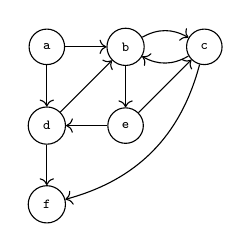
\begin{tikzpicture}[]
\node[draw, circle] (a) at (0, 0) {\tiny \texttt{a}};
\node[draw, circle] (b) at (1, 0) {\tiny \texttt{b}};
\node[draw, circle] (c) at (2, 0) {\tiny \texttt{c}};
\node[draw, circle] (e) at (1, -1) {\tiny \texttt{e}};
\node[draw, circle] (f) at (0, -2) {\tiny \texttt{f}};
\node[draw, circle] (d) at (0, -1) {\tiny \texttt{d}};

\draw[->] (a) -- (b);
\draw[->] (b) edge[bend left] (c);
\draw[->] (b) -- (e);
\draw[->] (c) edge[bend left] (f);
\draw[->] (e) -- (d);


\draw[->] (c) edge[bend left] (b);
\draw[->] (d) edge[] (b);

\draw[->] (a) edge[] (d);
\draw[->] (e) edge[] (c);
\draw[->] (d) edge[] (f);
\end{tikzpicture}

&

\quad

&

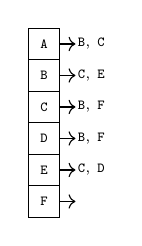
\begin{tikzpicture}[scale = 0.4]
\draw (0, 0) grid (1, 6);
\node at (0.5, 0.5) {\tiny \texttt{F}};
\node at (0.5, 1.5) {\tiny \texttt{E}};
\node at (0.5, 2.5) {\tiny \texttt{D}};
\node at (0.5, 3.5) {\tiny \texttt{C}};
\node at (0.5, 4.5) {\tiny \texttt{B}};
\node at (0.5, 5.5) {\tiny \texttt{A}};

\draw[->] (1, 0.5) -- (1.5, 0.5);
\draw[->] (1, 1.5) -- (1.5, 1.5);
\draw[->] (1, 2.5) -- (1.5, 2.5);
\draw[->] (1, 3.5) -- (1.5, 3.5);
\draw[->] (1, 4.5) -- (1.5, 4.5);
\draw[->] (1, 5.5) -- (1.5, 5.5);


\node at (2, 5.5) {\tiny \texttt{B}, \texttt{C}};
\node at (2, 4.5) {\tiny \texttt{C}, \texttt{E}};
\node at (2, 3.5) {\tiny \texttt{B}, \texttt{F}};
\node at (2, 2.5) {\tiny \texttt{B}, \texttt{F}};
\node at (2, 1.5) {\tiny \texttt{C}, \texttt{D}};
\end{tikzpicture}

\end{tabular}
\end{center}

DFS execution from node \texttt{a}

\begin{center}
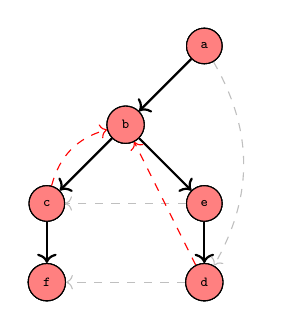
\begin{tikzpicture}[]

\node[draw, circle] (a) at (0, 0) {\tiny \texttt{a}};

\pause

\node[draw, fill = green!50!white, circle] (a) at (0, 0) {\tiny \texttt{a}};

\pause

\node[draw, circle] (b) at (-1, -1) {\tiny \texttt{b}};
\draw[->, thick] (a) -- (b);

\pause

\node[draw, fill = green!50!white, circle] (b) at (-1, -1) {\tiny \texttt{b}};

\pause

\node[draw, circle] (c) at (-2, -2) {\tiny \texttt{c}};
\draw[->, thick] (b) -- (c);

\pause 

\node[draw, fill = green!50!white, circle] (c) at (-2, -2) {\tiny \texttt{c}};

\pause

\draw[->, dashed, red] (c) edge[bend left] (b);

\pause

\node[draw, circle] (f) at (-2, -3) {\tiny \texttt{f}};
\draw[->, thick] (c) -- (f);

\pause

\node[draw, fill = green!50!white, circle] (f) at (-2, -3) {\tiny \texttt{f}};

\pause

\node[draw, fill = red!50!white, circle] (f) at (-2, -3) {\tiny \texttt{f}};

\pause

\node[draw, fill = red!50!white, circle] (c) at (-2, -2) {\tiny \texttt{c}};

\pause

\node[draw, circle] (e) at (0, -2) {\tiny \texttt{e}};
\draw[->, thick] (b) -- (e);

\pause

\node[draw, fill = green!50!white, circle] (e) at (0, -2) {\tiny \texttt{e}};

\pause

\draw[->, dashed, gray!50!white] (e) edge[] (c);

\pause

\node[draw, circle] (d) at (0, -3) {\tiny \texttt{d}};
\draw[->, thick] (e) -- (d);

\pause

\node[draw, fill = green!50!white, circle] (d) at (0, -3) {\tiny \texttt{d}};

\pause

\draw[->, dashed, red] (d) edge[] (b);

\pause 

\draw[->, dashed, gray!50!white] (d) edge[] (f);

\pause

\node[draw, fill = red!50!white, circle] (d) at (0, -3) {\tiny \texttt{d}};

\pause

\node[draw, fill = red!50!white, circle] (e) at (0, -2) {\tiny \texttt{e}};

\pause

\node[draw, fill = red!50!white, circle] (b) at (-1, -1) {\tiny \texttt{b}};

\pause

\draw[->, dashed, gray!50!white] (a) edge[bend left] (d);

\pause


\node[draw, fill = red!50!white, circle] (a) at (0, 0) {\tiny \texttt{a}};



\end{tikzpicture}
\end{center}

\end{frame}



\section{BFS}

\begin{frame}{What is a BFS ?}
BFS stands for Breadth First Search. It is an algorithm used to compute distance and shortest path on unweighed graphs.\\
\vspace{0.5cm}
This algorithm uses a \textbf{queue} datastucture ( first-in, first-out).\\

\begin{figure}
\begin{tikzpicture}
    \node[draw, shape=rectangle, minimum width=0.6cm, minimum height=1.5cm] (a1) at (-1,0) {4};
   	\node[draw, shape=rectangle, minimum width=0.6cm, minimum height=1.5cm] (a2) at (0,0) {3};
   	\node[draw, shape=rectangle, minimum width=0.6cm, minimum height=1.5cm] (a3) at (1,0) {2};
   	\node[draw, shape=rectangle, minimum width=0.6cm, minimum height=1.5cm] (a4) at (2,0) {1};
   	
   	\node[draw, shape=rectangle, minimum width=0.6cm, minimum height=1.5cm] (a0) at (-4,1) {5};
   	\node[draw, shape=rectangle, minimum width=0.6cm, minimum height=1.5cm] (a5) at (5,-1) {0};
   	

   	\path[->] (a4) edge [out=0, in=180] (a5) node[right=1cm] {\ci{pop()}};
	\path[->] (a0) edge [out=0, in=180] (a1) node[right=1cm] {\ci{push()}};
	
	\path[->] (a1) edge (a2);
   	\path[->] (a2) edge (a3);
   	\path[->] (a3) edge (a4);

\end{tikzpicture}
\end{figure}

\end{frame}

\begin{frame}{BFS : Algorithm}
Star by putting the first vertex in the queue add set its distance to be $0$, set all nodes as unvisited (distance $= \infty$). Then as long as the queue is not empty :
\begin{itemize}
\item Poll the first vertex in the queue.
\item For each of its unvisited (distance $= \infty$) neighbour :\\
\begin{itemize}
	\item Otherwise, set its distance as the distance of the polled vertex + 1 and add it to the queue.
	\item Set the parent of the neighbour as the current vertex.
\end{itemize}
\end{itemize}
To track the shortest path, begin at the destination and go up from parent to parent until reaching the starting vertex.
\end{frame}

\begin{frame}{BFS : Code}
  \src{bfs.cpp}
\end{frame}

\begin{frame}{BFS : Example}
\begin{figure}
\vspace*{-1cm} 
\center
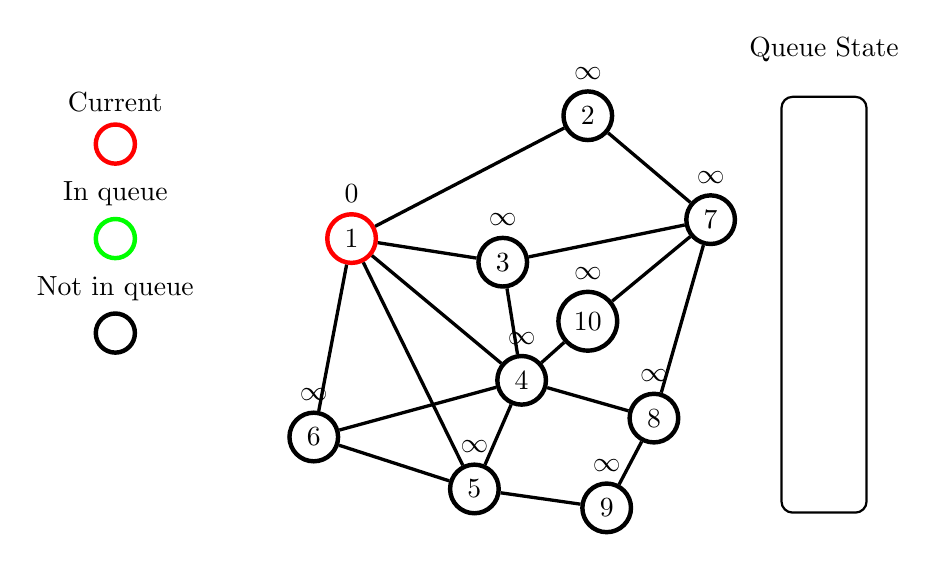
\begin{tikzpicture}[scale=1.2] 
\node[shape=circle, draw=red, 	ultra thick, scale=1.5pt, label={Current}] (U) at (-2.5, 1) {}; 
\node[shape=circle, draw=green,  ultra thick, scale=1.5pt, label={In queue}] (U) at (-2.5, 0) {}; 
\node[shape=circle, draw=black, ultra thick, scale=1.5pt, label={Not in queue}] (U) at (-2.5, -1) {}; 
\draw[thick, rounded corners,draw=black] (4.55, 1.5) rectangle ++(0.9, -1-4*0.85 );
\node[draw=white] at (5, 2) {Queue State} ; 
\node[shape=circle,draw=red, ultra thick, label={$0$}] (1) at (0,0) {1}; 
\node[shape=circle,draw=black, ultra thick, label={$\infty$}] (2) at (2.5,1.3) {2}; 
\node[shape=circle,draw=black, ultra thick, label={$\infty$}] (3) at (1.6,-0.25) {3}; 
\node[shape=circle,draw=black, ultra thick, label={$\infty$}] (4) at (1.8,-1.5) {4}; 
\node[shape=circle,draw=black, ultra thick, label={$\infty$}] (5) at (1.3,-2.65) {5}; 
\node[shape=circle,draw=black, ultra thick, label={$\infty$}] (6) at (-0.4,-2.1) {6}; 
\node[shape=circle,draw=black, ultra thick, label={$\infty$}] (7) at (3.8,0.2) {7}; 
\node[shape=circle,draw=black, ultra thick, label={$\infty$}] (8) at (3.2,-1.9) {8}; 
\node[shape=circle,draw=black, ultra thick, label={$\infty$}] (9) at (2.7,-2.85) {9}; 
\node[shape=circle,draw=black, ultra thick, label={$\infty$}] (10) at (2.5,-0.875) {10}; 
\path [-,very thick, draw=black] (1) edge  (2);
\path [-,very thick, draw=black] (1) edge  (3);
\path [-,very thick, draw=black] (1) edge  (4);
\path [-,very thick, draw=black] (1) edge  (5);
\path [-,very thick, draw=black] (1) edge  (6);
\path [-,very thick, draw=black] (2) edge  (7);
\path [-,very thick, draw=black] (3) edge  (7);
\path [-,very thick, draw=black] (3) edge  (4);
\path [-,very thick, draw=black] (4) edge  (5);
\path [-,very thick, draw=black] (4) edge  (6);
\path [-,very thick, draw=black] (4) edge  (8);
\path [-,very thick, draw=black] (4) edge  (10);
\path [-,very thick, draw=black] (5) edge  (6);
\path [-,very thick, draw=black] (5) edge  (9);
\path [-,very thick, draw=black] (7) edge  (8);
\path [-,very thick, draw=black] (7) edge  (10);
\path [-,very thick, draw=black] (8) edge  (9);
\end{tikzpicture} 
\end{figure} 
\end{frame} 
\begin{frame}{BFS : Example}
\begin{figure}
\vspace*{-1cm} 
\center
\begin{tikzpicture}[scale=1.2] 
\node[shape=circle, draw=red, 	ultra thick, scale=1.5pt, label={Current}] (U) at (-2.5, 1) {}; 
\node[shape=circle, draw=green,  ultra thick, scale=1.5pt, label={In queue}] (U) at (-2.5, 0) {}; 
\node[shape=circle, draw=black, ultra thick, scale=1.5pt, label={Not in queue}] (U) at (-2.5, -1) {}; 
\draw[thick, rounded corners,draw=black] (4.55, 1.5) rectangle ++(0.9, -1-4*0.85 );
\node[draw=white] at (5, 2) {Queue State} ; 
\node[shape=circle, draw=black, thick, minimum size=2pt] (U0) at (5, 1.0) {\tiny{2}}; 
\path[->, thick, draw=black] (2) edge [dashed, bend right=30] (U0); 
\node[shape=circle,draw=red, ultra thick, label={$0$}] (1) at (0,0) {1}; 
\node[shape=circle,draw=green, ultra thick, label={$1$}] (2) at (2.5,1.3) {2}; 
\node[shape=circle,draw=black, ultra thick, label={$\infty$}] (3) at (1.6,-0.25) {3}; 
\node[shape=circle,draw=black, ultra thick, label={$\infty$}] (4) at (1.8,-1.5) {4}; 
\node[shape=circle,draw=black, ultra thick, label={$\infty$}] (5) at (1.3,-2.65) {5}; 
\node[shape=circle,draw=black, ultra thick, label={$\infty$}] (6) at (-0.4,-2.1) {6}; 
\node[shape=circle,draw=black, ultra thick, label={$\infty$}] (7) at (3.8,0.2) {7}; 
\node[shape=circle,draw=black, ultra thick, label={$\infty$}] (8) at (3.2,-1.9) {8}; 
\node[shape=circle,draw=black, ultra thick, label={$\infty$}] (9) at (2.7,-2.85) {9}; 
\node[shape=circle,draw=black, ultra thick, label={$\infty$}] (10) at (2.5,-0.875) {10}; 
\path [->,very thick, draw=red] (1) edge  (2);
\path [-,very thick, draw=black] (1) edge  (3);
\path [-,very thick, draw=black] (1) edge  (4);
\path [-,very thick, draw=black] (1) edge  (5);
\path [-,very thick, draw=black] (1) edge  (6);
\path [-,very thick, draw=black] (2) edge  (7);
\path [-,very thick, draw=black] (3) edge  (7);
\path [-,very thick, draw=black] (3) edge  (4);
\path [-,very thick, draw=black] (4) edge  (5);
\path [-,very thick, draw=black] (4) edge  (6);
\path [-,very thick, draw=black] (4) edge  (8);
\path [-,very thick, draw=black] (4) edge  (10);
\path [-,very thick, draw=black] (5) edge  (6);
\path [-,very thick, draw=black] (5) edge  (9);
\path [-,very thick, draw=black] (7) edge  (8);
\path [-,very thick, draw=black] (7) edge  (10);
\path [-,very thick, draw=black] (8) edge  (9);
\end{tikzpicture} 
\end{figure} 
\end{frame} 
\begin{frame}{BFS : Example}
\begin{figure}
\vspace*{-1cm} 
\center
\begin{tikzpicture}[scale=1.2] 
\node[shape=circle, draw=red, 	ultra thick, scale=1.5pt, label={Current}] (U) at (-2.5, 1) {}; 
\node[shape=circle, draw=green,  ultra thick, scale=1.5pt, label={In queue}] (U) at (-2.5, 0) {}; 
\node[shape=circle, draw=black, ultra thick, scale=1.5pt, label={Not in queue}] (U) at (-2.5, -1) {}; 
\draw[thick, rounded corners,draw=black] (4.55, 1.5) rectangle ++(0.9, -1-4*0.85 );
\node[draw=white] at (5, 2) {Queue State} ; 
\node[shape=circle, draw=black, thick, minimum size=2pt] (U0) at (5, 1.0) {\tiny{2}}; 
\node[shape=circle, draw=black, thick, minimum size=2pt] (U1) at (5, 0.15000000000000002) {\tiny{3}}; 
\path[->] (U1) edge [out=75, in=-75] (U0);
\path[->, thick, draw=black] (3) edge [dashed, bend right=30] (U1); 
\node[shape=circle,draw=red, ultra thick, label={$0$}] (1) at (0,0) {1}; 
\node[shape=circle,draw=green, ultra thick, label={$1$}] (2) at (2.5,1.3) {2}; 
\node[shape=circle,draw=green, ultra thick, label={$1$}] (3) at (1.6,-0.25) {3}; 
\node[shape=circle,draw=black, ultra thick, label={$\infty$}] (4) at (1.8,-1.5) {4}; 
\node[shape=circle,draw=black, ultra thick, label={$\infty$}] (5) at (1.3,-2.65) {5}; 
\node[shape=circle,draw=black, ultra thick, label={$\infty$}] (6) at (-0.4,-2.1) {6}; 
\node[shape=circle,draw=black, ultra thick, label={$\infty$}] (7) at (3.8,0.2) {7}; 
\node[shape=circle,draw=black, ultra thick, label={$\infty$}] (8) at (3.2,-1.9) {8}; 
\node[shape=circle,draw=black, ultra thick, label={$\infty$}] (9) at (2.7,-2.85) {9}; 
\node[shape=circle,draw=black, ultra thick, label={$\infty$}] (10) at (2.5,-0.875) {10}; 
\path [-,very thick, draw=black] (1) edge  (2);
\path [->,very thick, draw=red] (1) edge  (3);
\path [-,very thick, draw=black] (1) edge  (4);
\path [-,very thick, draw=black] (1) edge  (5);
\path [-,very thick, draw=black] (1) edge  (6);
\path [-,very thick, draw=black] (2) edge  (7);
\path [-,very thick, draw=black] (3) edge  (7);
\path [-,very thick, draw=black] (3) edge  (4);
\path [-,very thick, draw=black] (4) edge  (5);
\path [-,very thick, draw=black] (4) edge  (6);
\path [-,very thick, draw=black] (4) edge  (8);
\path [-,very thick, draw=black] (4) edge  (10);
\path [-,very thick, draw=black] (5) edge  (6);
\path [-,very thick, draw=black] (5) edge  (9);
\path [-,very thick, draw=black] (7) edge  (8);
\path [-,very thick, draw=black] (7) edge  (10);
\path [-,very thick, draw=black] (8) edge  (9);
\end{tikzpicture} 
\end{figure} 
\end{frame} 
\begin{frame}{BFS : Example}
\begin{figure}
\vspace*{-1cm} 
\center
\begin{tikzpicture}[scale=1.2] 
\node[shape=circle, draw=red, 	ultra thick, scale=1.5pt, label={Current}] (U) at (-2.5, 1) {}; 
\node[shape=circle, draw=green,  ultra thick, scale=1.5pt, label={In queue}] (U) at (-2.5, 0) {}; 
\node[shape=circle, draw=black, ultra thick, scale=1.5pt, label={Not in queue}] (U) at (-2.5, -1) {}; 
\draw[thick, rounded corners,draw=black] (4.55, 1.5) rectangle ++(0.9, -1-4*0.85 );
\node[draw=white] at (5, 2) {Queue State} ; 
\node[shape=circle, draw=black, thick, minimum size=2pt] (U0) at (5, 1.0) {\tiny{2}}; 
\node[shape=circle, draw=black, thick, minimum size=2pt] (U1) at (5, 0.15000000000000002) {\tiny{3}}; 
\node[shape=circle, draw=black, thick, minimum size=2pt] (U2) at (5, -0.7) {\tiny{4}}; 
\path[->] (U1) edge [out=75, in=-75] (U0);
\path[->] (U2) edge [out=75, in=-75] (U1);
\path[->, thick, draw=black] (4) edge [dashed, bend right=30] (U2); 
\node[shape=circle,draw=red, ultra thick, label={$0$}] (1) at (0,0) {1}; 
\node[shape=circle,draw=green, ultra thick, label={$1$}] (2) at (2.5,1.3) {2}; 
\node[shape=circle,draw=green, ultra thick, label={$1$}] (3) at (1.6,-0.25) {3}; 
\node[shape=circle,draw=green, ultra thick, label={$1$}] (4) at (1.8,-1.5) {4}; 
\node[shape=circle,draw=black, ultra thick, label={$\infty$}] (5) at (1.3,-2.65) {5}; 
\node[shape=circle,draw=black, ultra thick, label={$\infty$}] (6) at (-0.4,-2.1) {6}; 
\node[shape=circle,draw=black, ultra thick, label={$\infty$}] (7) at (3.8,0.2) {7}; 
\node[shape=circle,draw=black, ultra thick, label={$\infty$}] (8) at (3.2,-1.9) {8}; 
\node[shape=circle,draw=black, ultra thick, label={$\infty$}] (9) at (2.7,-2.85) {9}; 
\node[shape=circle,draw=black, ultra thick, label={$\infty$}] (10) at (2.5,-0.875) {10}; 
\path [-,very thick, draw=black] (1) edge  (2);
\path [-,very thick, draw=black] (1) edge  (3);
\path [->,very thick, draw=red] (1) edge  (4);
\path [-,very thick, draw=black] (1) edge  (5);
\path [-,very thick, draw=black] (1) edge  (6);
\path [-,very thick, draw=black] (2) edge  (7);
\path [-,very thick, draw=black] (3) edge  (7);
\path [-,very thick, draw=black] (3) edge  (4);
\path [-,very thick, draw=black] (4) edge  (5);
\path [-,very thick, draw=black] (4) edge  (6);
\path [-,very thick, draw=black] (4) edge  (8);
\path [-,very thick, draw=black] (4) edge  (10);
\path [-,very thick, draw=black] (5) edge  (6);
\path [-,very thick, draw=black] (5) edge  (9);
\path [-,very thick, draw=black] (7) edge  (8);
\path [-,very thick, draw=black] (7) edge  (10);
\path [-,very thick, draw=black] (8) edge  (9);
\end{tikzpicture} 
\end{figure} 
\end{frame} 
\begin{frame}{BFS : Example}
\begin{figure}
\vspace*{-1cm} 
\center
\begin{tikzpicture}[scale=1.2] 
\node[shape=circle, draw=red, 	ultra thick, scale=1.5pt, label={Current}] (U) at (-2.5, 1) {}; 
\node[shape=circle, draw=green,  ultra thick, scale=1.5pt, label={In queue}] (U) at (-2.5, 0) {}; 
\node[shape=circle, draw=black, ultra thick, scale=1.5pt, label={Not in queue}] (U) at (-2.5, -1) {}; 
\draw[thick, rounded corners,draw=black] (4.55, 1.5) rectangle ++(0.9, -1-4*0.85 );
\node[draw=white] at (5, 2) {Queue State} ; 
\node[shape=circle, draw=black, thick, minimum size=2pt] (U0) at (5, 1.0) {\tiny{2}}; 
\node[shape=circle, draw=black, thick, minimum size=2pt] (U1) at (5, 0.15000000000000002) {\tiny{3}}; 
\node[shape=circle, draw=black, thick, minimum size=2pt] (U2) at (5, -0.7) {\tiny{4}}; 
\node[shape=circle, draw=black, thick, minimum size=2pt] (U3) at (5, -1.5499999999999998) {\tiny{5}}; 
\path[->] (U1) edge [out=75, in=-75] (U0);
\path[->] (U2) edge [out=75, in=-75] (U1);
\path[->] (U3) edge [out=75, in=-75] (U2);
\path[->, thick, draw=black] (5) edge [dashed, bend right=30] (U3); 
\node[shape=circle,draw=red, ultra thick, label={$0$}] (1) at (0,0) {1}; 
\node[shape=circle,draw=green, ultra thick, label={$1$}] (2) at (2.5,1.3) {2}; 
\node[shape=circle,draw=green, ultra thick, label={$1$}] (3) at (1.6,-0.25) {3}; 
\node[shape=circle,draw=green, ultra thick, label={$1$}] (4) at (1.8,-1.5) {4}; 
\node[shape=circle,draw=green, ultra thick, label={$1$}] (5) at (1.3,-2.65) {5}; 
\node[shape=circle,draw=black, ultra thick, label={$\infty$}] (6) at (-0.4,-2.1) {6}; 
\node[shape=circle,draw=black, ultra thick, label={$\infty$}] (7) at (3.8,0.2) {7}; 
\node[shape=circle,draw=black, ultra thick, label={$\infty$}] (8) at (3.2,-1.9) {8}; 
\node[shape=circle,draw=black, ultra thick, label={$\infty$}] (9) at (2.7,-2.85) {9}; 
\node[shape=circle,draw=black, ultra thick, label={$\infty$}] (10) at (2.5,-0.875) {10}; 
\path [-,very thick, draw=black] (1) edge  (2);
\path [-,very thick, draw=black] (1) edge  (3);
\path [-,very thick, draw=black] (1) edge  (4);
\path [->,very thick, draw=red] (1) edge  (5);
\path [-,very thick, draw=black] (1) edge  (6);
\path [-,very thick, draw=black] (2) edge  (7);
\path [-,very thick, draw=black] (3) edge  (7);
\path [-,very thick, draw=black] (3) edge  (4);
\path [-,very thick, draw=black] (4) edge  (5);
\path [-,very thick, draw=black] (4) edge  (6);
\path [-,very thick, draw=black] (4) edge  (8);
\path [-,very thick, draw=black] (4) edge  (10);
\path [-,very thick, draw=black] (5) edge  (6);
\path [-,very thick, draw=black] (5) edge  (9);
\path [-,very thick, draw=black] (7) edge  (8);
\path [-,very thick, draw=black] (7) edge  (10);
\path [-,very thick, draw=black] (8) edge  (9);
\end{tikzpicture} 
\end{figure} 
\end{frame} 
\begin{frame}{BFS : Example}
\begin{figure}
\vspace*{-1cm} 
\center
\begin{tikzpicture}[scale=1.2] 
\node[shape=circle, draw=red, 	ultra thick, scale=1.5pt, label={Current}] (U) at (-2.5, 1) {}; 
\node[shape=circle, draw=green,  ultra thick, scale=1.5pt, label={In queue}] (U) at (-2.5, 0) {}; 
\node[shape=circle, draw=black, ultra thick, scale=1.5pt, label={Not in queue}] (U) at (-2.5, -1) {}; 
\draw[thick, rounded corners,draw=black] (4.55, 1.5) rectangle ++(0.9, -1-4*0.85 );
\node[draw=white] at (5, 2) {Queue State} ; 
\node[shape=circle, draw=black, thick, minimum size=2pt] (U0) at (5, 1.0) {\tiny{2}}; 
\node[shape=circle, draw=black, thick, minimum size=2pt] (U1) at (5, 0.15000000000000002) {\tiny{3}}; 
\node[shape=circle, draw=black, thick, minimum size=2pt] (U2) at (5, -0.7) {\tiny{4}}; 
\node[shape=circle, draw=black, thick, minimum size=2pt] (U3) at (5, -1.5499999999999998) {\tiny{5}}; 
\node[shape=circle, draw=black, thick, minimum size=2pt] (U4) at (5, -2.4) {\tiny{6}}; 
\path[->] (U1) edge [out=75, in=-75] (U0);
\path[->] (U2) edge [out=75, in=-75] (U1);
\path[->] (U3) edge [out=75, in=-75] (U2);
\path[->] (U4) edge [out=75, in=-75] (U3);
\path[->, thick, draw=black] (6) edge [dashed, bend right=30] (U4); 
\node[shape=circle,draw=red, ultra thick, label={$0$}] (1) at (0,0) {1}; 
\node[shape=circle,draw=green, ultra thick, label={$1$}] (2) at (2.5,1.3) {2}; 
\node[shape=circle,draw=green, ultra thick, label={$1$}] (3) at (1.6,-0.25) {3}; 
\node[shape=circle,draw=green, ultra thick, label={$1$}] (4) at (1.8,-1.5) {4}; 
\node[shape=circle,draw=green, ultra thick, label={$1$}] (5) at (1.3,-2.65) {5}; 
\node[shape=circle,draw=green, ultra thick, label={$1$}] (6) at (-0.4,-2.1) {6}; 
\node[shape=circle,draw=black, ultra thick, label={$\infty$}] (7) at (3.8,0.2) {7}; 
\node[shape=circle,draw=black, ultra thick, label={$\infty$}] (8) at (3.2,-1.9) {8}; 
\node[shape=circle,draw=black, ultra thick, label={$\infty$}] (9) at (2.7,-2.85) {9}; 
\node[shape=circle,draw=black, ultra thick, label={$\infty$}] (10) at (2.5,-0.875) {10}; 
\path [-,very thick, draw=black] (1) edge  (2);
\path [-,very thick, draw=black] (1) edge  (3);
\path [-,very thick, draw=black] (1) edge  (4);
\path [-,very thick, draw=black] (1) edge  (5);
\path [->,very thick, draw=red] (1) edge  (6);
\path [-,very thick, draw=black] (2) edge  (7);
\path [-,very thick, draw=black] (3) edge  (7);
\path [-,very thick, draw=black] (3) edge  (4);
\path [-,very thick, draw=black] (4) edge  (5);
\path [-,very thick, draw=black] (4) edge  (6);
\path [-,very thick, draw=black] (4) edge  (8);
\path [-,very thick, draw=black] (4) edge  (10);
\path [-,very thick, draw=black] (5) edge  (6);
\path [-,very thick, draw=black] (5) edge  (9);
\path [-,very thick, draw=black] (7) edge  (8);
\path [-,very thick, draw=black] (7) edge  (10);
\path [-,very thick, draw=black] (8) edge  (9);
\end{tikzpicture} 
\end{figure} 
\end{frame} 
\begin{frame}{BFS : Example}
\begin{figure}
\vspace*{-1cm} 
\center
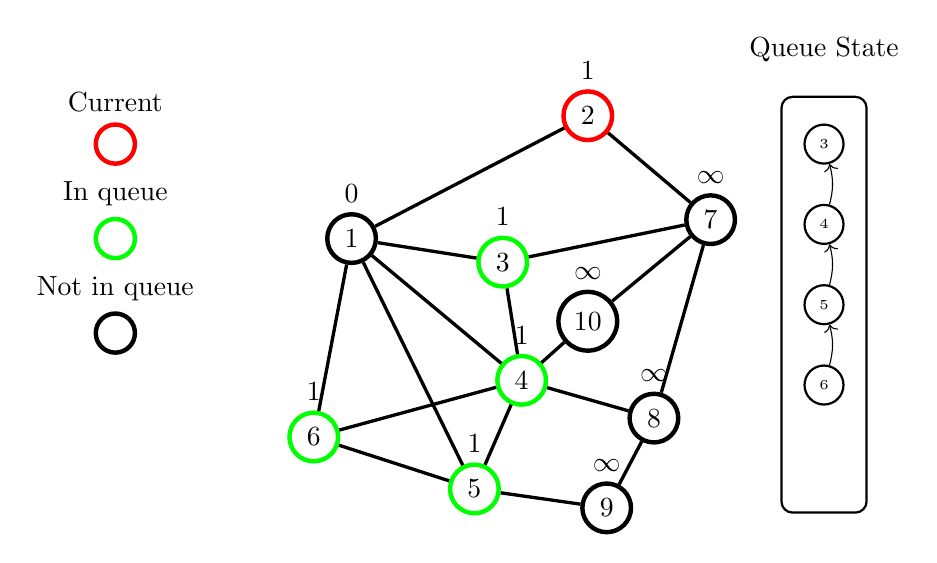
\begin{tikzpicture}[scale=1.2] 
\node[shape=circle, draw=red, 	ultra thick, scale=1.5pt, label={Current}] (U) at (-2.5, 1) {}; 
\node[shape=circle, draw=green,  ultra thick, scale=1.5pt, label={In queue}] (U) at (-2.5, 0) {}; 
\node[shape=circle, draw=black, ultra thick, scale=1.5pt, label={Not in queue}] (U) at (-2.5, -1) {}; 
\draw[thick, rounded corners,draw=black] (4.55, 1.5) rectangle ++(0.9, -1-4*0.85 );
\node[draw=white] at (5, 2) {Queue State} ; 
\node[shape=circle, draw=black, thick, minimum size=2pt] (U0) at (5, 1.0) {\tiny{3}}; 
\node[shape=circle, draw=black, thick, minimum size=2pt] (U1) at (5, 0.15000000000000002) {\tiny{4}}; 
\node[shape=circle, draw=black, thick, minimum size=2pt] (U2) at (5, -0.7) {\tiny{5}}; 
\node[shape=circle, draw=black, thick, minimum size=2pt] (U3) at (5, -1.5499999999999998) {\tiny{6}}; 
\path[->] (U1) edge [out=75, in=-75] (U0);
\path[->] (U2) edge [out=75, in=-75] (U1);
\path[->] (U3) edge [out=75, in=-75] (U2);
\node[shape=circle,draw=black, ultra thick, label={$0$}] (1) at (0,0) {1}; 
\node[shape=circle,draw=red, ultra thick, label={$1$}] (2) at (2.5,1.3) {2}; 
\node[shape=circle,draw=green, ultra thick, label={$1$}] (3) at (1.6,-0.25) {3}; 
\node[shape=circle,draw=green, ultra thick, label={$1$}] (4) at (1.8,-1.5) {4}; 
\node[shape=circle,draw=green, ultra thick, label={$1$}] (5) at (1.3,-2.65) {5}; 
\node[shape=circle,draw=green, ultra thick, label={$1$}] (6) at (-0.4,-2.1) {6}; 
\node[shape=circle,draw=black, ultra thick, label={$\infty$}] (7) at (3.8,0.2) {7}; 
\node[shape=circle,draw=black, ultra thick, label={$\infty$}] (8) at (3.2,-1.9) {8}; 
\node[shape=circle,draw=black, ultra thick, label={$\infty$}] (9) at (2.7,-2.85) {9}; 
\node[shape=circle,draw=black, ultra thick, label={$\infty$}] (10) at (2.5,-0.875) {10}; 
\path [-,very thick, draw=black] (1) edge  (2);
\path [-,very thick, draw=black] (1) edge  (3);
\path [-,very thick, draw=black] (1) edge  (4);
\path [-,very thick, draw=black] (1) edge  (5);
\path [-,very thick, draw=black] (1) edge  (6);
\path [-,very thick, draw=black] (2) edge  (7);
\path [-,very thick, draw=black] (3) edge  (7);
\path [-,very thick, draw=black] (3) edge  (4);
\path [-,very thick, draw=black] (4) edge  (5);
\path [-,very thick, draw=black] (4) edge  (6);
\path [-,very thick, draw=black] (4) edge  (8);
\path [-,very thick, draw=black] (4) edge  (10);
\path [-,very thick, draw=black] (5) edge  (6);
\path [-,very thick, draw=black] (5) edge  (9);
\path [-,very thick, draw=black] (7) edge  (8);
\path [-,very thick, draw=black] (7) edge  (10);
\path [-,very thick, draw=black] (8) edge  (9);
\end{tikzpicture} 
\end{figure} 
\end{frame} 
\begin{frame}{BFS : Example}
\begin{figure}
\vspace*{-1cm} 
\center
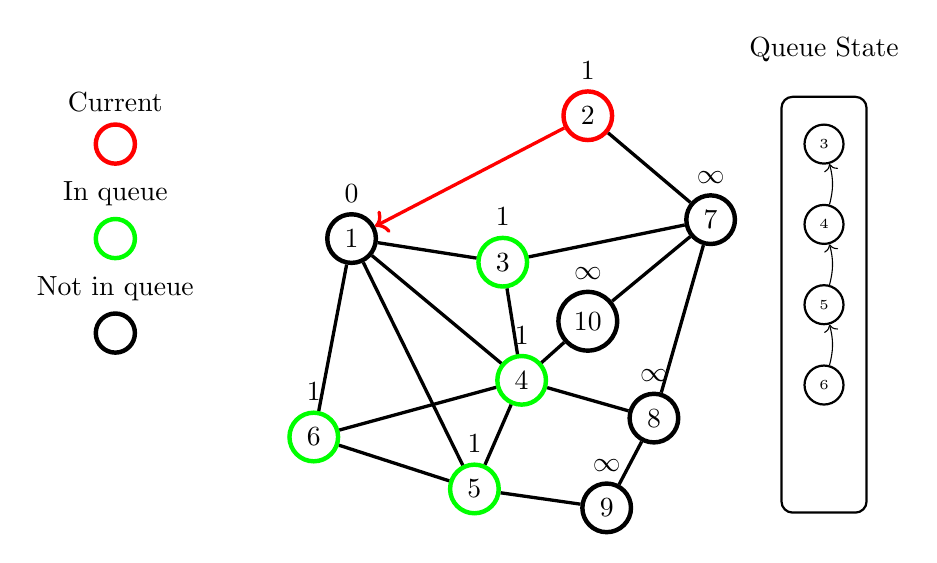
\begin{tikzpicture}[scale=1.2] 
\node[shape=circle, draw=red, 	ultra thick, scale=1.5pt, label={Current}] (U) at (-2.5, 1) {}; 
\node[shape=circle, draw=green,  ultra thick, scale=1.5pt, label={In queue}] (U) at (-2.5, 0) {}; 
\node[shape=circle, draw=black, ultra thick, scale=1.5pt, label={Not in queue}] (U) at (-2.5, -1) {}; 
\draw[thick, rounded corners,draw=black] (4.55, 1.5) rectangle ++(0.9, -1-4*0.85 );
\node[draw=white] at (5, 2) {Queue State} ; 
\node[shape=circle, draw=black, thick, minimum size=2pt] (U0) at (5, 1.0) {\tiny{3}}; 
\node[shape=circle, draw=black, thick, minimum size=2pt] (U1) at (5, 0.15000000000000002) {\tiny{4}}; 
\node[shape=circle, draw=black, thick, minimum size=2pt] (U2) at (5, -0.7) {\tiny{5}}; 
\node[shape=circle, draw=black, thick, minimum size=2pt] (U3) at (5, -1.5499999999999998) {\tiny{6}}; 
\path[->] (U1) edge [out=75, in=-75] (U0);
\path[->] (U2) edge [out=75, in=-75] (U1);
\path[->] (U3) edge [out=75, in=-75] (U2);
\node[shape=circle,draw=black, ultra thick, label={$0$}] (1) at (0,0) {1}; 
\node[shape=circle,draw=red, ultra thick, label={$1$}] (2) at (2.5,1.3) {2}; 
\node[shape=circle,draw=green, ultra thick, label={$1$}] (3) at (1.6,-0.25) {3}; 
\node[shape=circle,draw=green, ultra thick, label={$1$}] (4) at (1.8,-1.5) {4}; 
\node[shape=circle,draw=green, ultra thick, label={$1$}] (5) at (1.3,-2.65) {5}; 
\node[shape=circle,draw=green, ultra thick, label={$1$}] (6) at (-0.4,-2.1) {6}; 
\node[shape=circle,draw=black, ultra thick, label={$\infty$}] (7) at (3.8,0.2) {7}; 
\node[shape=circle,draw=black, ultra thick, label={$\infty$}] (8) at (3.2,-1.9) {8}; 
\node[shape=circle,draw=black, ultra thick, label={$\infty$}] (9) at (2.7,-2.85) {9}; 
\node[shape=circle,draw=black, ultra thick, label={$\infty$}] (10) at (2.5,-0.875) {10}; 
\path [->,very thick, draw=red] (2) edge  (1);
\path [-,very thick, draw=black] (1) edge  (3);
\path [-,very thick, draw=black] (1) edge  (4);
\path [-,very thick, draw=black] (1) edge  (5);
\path [-,very thick, draw=black] (1) edge  (6);
\path [-,very thick, draw=black] (2) edge  (7);
\path [-,very thick, draw=black] (3) edge  (7);
\path [-,very thick, draw=black] (3) edge  (4);
\path [-,very thick, draw=black] (4) edge  (5);
\path [-,very thick, draw=black] (4) edge  (6);
\path [-,very thick, draw=black] (4) edge  (8);
\path [-,very thick, draw=black] (4) edge  (10);
\path [-,very thick, draw=black] (5) edge  (6);
\path [-,very thick, draw=black] (5) edge  (9);
\path [-,very thick, draw=black] (7) edge  (8);
\path [-,very thick, draw=black] (7) edge  (10);
\path [-,very thick, draw=black] (8) edge  (9);
\end{tikzpicture} 
\end{figure} 
\end{frame} 
\begin{frame}{BFS : Example}
\begin{figure}
\vspace*{-1cm} 
\center
\begin{tikzpicture}[scale=1.2] 
\node[shape=circle, draw=red, 	ultra thick, scale=1.5pt, label={Current}] (U) at (-2.5, 1) {}; 
\node[shape=circle, draw=green,  ultra thick, scale=1.5pt, label={In queue}] (U) at (-2.5, 0) {}; 
\node[shape=circle, draw=black, ultra thick, scale=1.5pt, label={Not in queue}] (U) at (-2.5, -1) {}; 
\draw[thick, rounded corners,draw=black] (4.55, 1.5) rectangle ++(0.9, -1-4*0.85 );
\node[draw=white] at (5, 2) {Queue State} ; 
\node[shape=circle, draw=black, thick, minimum size=2pt] (U0) at (5, 1.0) {\tiny{3}}; 
\node[shape=circle, draw=black, thick, minimum size=2pt] (U1) at (5, 0.15000000000000002) {\tiny{4}}; 
\node[shape=circle, draw=black, thick, minimum size=2pt] (U2) at (5, -0.7) {\tiny{5}}; 
\node[shape=circle, draw=black, thick, minimum size=2pt] (U3) at (5, -1.5499999999999998) {\tiny{6}}; 
\node[shape=circle, draw=black, thick, minimum size=2pt] (U4) at (5, -2.4) {\tiny{7}}; 
\path[->] (U1) edge [out=75, in=-75] (U0);
\path[->] (U2) edge [out=75, in=-75] (U1);
\path[->] (U3) edge [out=75, in=-75] (U2);
\path[->] (U4) edge [out=75, in=-75] (U3);
\path[->, thick, draw=black] (7) edge [dashed, bend right=30] (U4); 
\node[shape=circle,draw=black, ultra thick, label={$0$}] (1) at (0,0) {1}; 
\node[shape=circle,draw=red, ultra thick, label={$1$}] (2) at (2.5,1.3) {2}; 
\node[shape=circle,draw=green, ultra thick, label={$1$}] (3) at (1.6,-0.25) {3}; 
\node[shape=circle,draw=green, ultra thick, label={$1$}] (4) at (1.8,-1.5) {4}; 
\node[shape=circle,draw=green, ultra thick, label={$1$}] (5) at (1.3,-2.65) {5}; 
\node[shape=circle,draw=green, ultra thick, label={$1$}] (6) at (-0.4,-2.1) {6}; 
\node[shape=circle,draw=green, ultra thick, label={$2$}] (7) at (3.8,0.2) {7}; 
\node[shape=circle,draw=black, ultra thick, label={$\infty$}] (8) at (3.2,-1.9) {8}; 
\node[shape=circle,draw=black, ultra thick, label={$\infty$}] (9) at (2.7,-2.85) {9}; 
\node[shape=circle,draw=black, ultra thick, label={$\infty$}] (10) at (2.5,-0.875) {10}; 
\path [-,very thick, draw=black] (1) edge  (2);
\path [-,very thick, draw=black] (1) edge  (3);
\path [-,very thick, draw=black] (1) edge  (4);
\path [-,very thick, draw=black] (1) edge  (5);
\path [-,very thick, draw=black] (1) edge  (6);
\path [->,very thick, draw=red] (2) edge  (7);
\path [-,very thick, draw=black] (3) edge  (7);
\path [-,very thick, draw=black] (3) edge  (4);
\path [-,very thick, draw=black] (4) edge  (5);
\path [-,very thick, draw=black] (4) edge  (6);
\path [-,very thick, draw=black] (4) edge  (8);
\path [-,very thick, draw=black] (4) edge  (10);
\path [-,very thick, draw=black] (5) edge  (6);
\path [-,very thick, draw=black] (5) edge  (9);
\path [-,very thick, draw=black] (7) edge  (8);
\path [-,very thick, draw=black] (7) edge  (10);
\path [-,very thick, draw=black] (8) edge  (9);
\end{tikzpicture} 
\end{figure} 
\end{frame} 
\begin{frame}{BFS : Example}
\begin{figure}
\vspace*{-1cm} 
\center
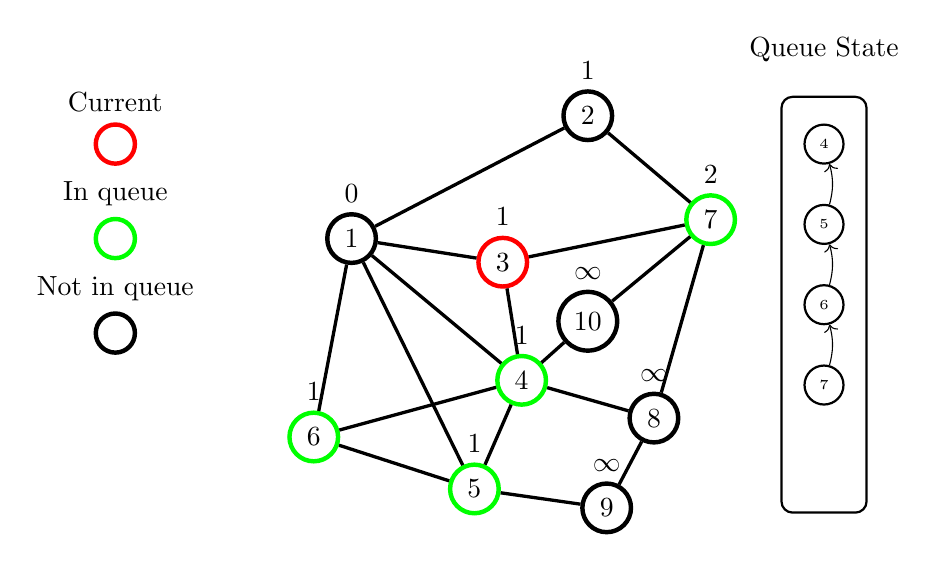
\begin{tikzpicture}[scale=1.2] 
\node[shape=circle, draw=red, 	ultra thick, scale=1.5pt, label={Current}] (U) at (-2.5, 1) {}; 
\node[shape=circle, draw=green,  ultra thick, scale=1.5pt, label={In queue}] (U) at (-2.5, 0) {}; 
\node[shape=circle, draw=black, ultra thick, scale=1.5pt, label={Not in queue}] (U) at (-2.5, -1) {}; 
\draw[thick, rounded corners,draw=black] (4.55, 1.5) rectangle ++(0.9, -1-4*0.85 );
\node[draw=white] at (5, 2) {Queue State} ; 
\node[shape=circle, draw=black, thick, minimum size=2pt] (U0) at (5, 1.0) {\tiny{4}}; 
\node[shape=circle, draw=black, thick, minimum size=2pt] (U1) at (5, 0.15000000000000002) {\tiny{5}}; 
\node[shape=circle, draw=black, thick, minimum size=2pt] (U2) at (5, -0.7) {\tiny{6}}; 
\node[shape=circle, draw=black, thick, minimum size=2pt] (U3) at (5, -1.5499999999999998) {\tiny{7}}; 
\path[->] (U1) edge [out=75, in=-75] (U0);
\path[->] (U2) edge [out=75, in=-75] (U1);
\path[->] (U3) edge [out=75, in=-75] (U2);
\node[shape=circle,draw=black, ultra thick, label={$0$}] (1) at (0,0) {1}; 
\node[shape=circle,draw=black, ultra thick, label={$1$}] (2) at (2.5,1.3) {2}; 
\node[shape=circle,draw=red, ultra thick, label={$1$}] (3) at (1.6,-0.25) {3}; 
\node[shape=circle,draw=green, ultra thick, label={$1$}] (4) at (1.8,-1.5) {4}; 
\node[shape=circle,draw=green, ultra thick, label={$1$}] (5) at (1.3,-2.65) {5}; 
\node[shape=circle,draw=green, ultra thick, label={$1$}] (6) at (-0.4,-2.1) {6}; 
\node[shape=circle,draw=green, ultra thick, label={$2$}] (7) at (3.8,0.2) {7}; 
\node[shape=circle,draw=black, ultra thick, label={$\infty$}] (8) at (3.2,-1.9) {8}; 
\node[shape=circle,draw=black, ultra thick, label={$\infty$}] (9) at (2.7,-2.85) {9}; 
\node[shape=circle,draw=black, ultra thick, label={$\infty$}] (10) at (2.5,-0.875) {10}; 
\path [-,very thick, draw=black] (1) edge  (2);
\path [-,very thick, draw=black] (1) edge  (3);
\path [-,very thick, draw=black] (1) edge  (4);
\path [-,very thick, draw=black] (1) edge  (5);
\path [-,very thick, draw=black] (1) edge  (6);
\path [-,very thick, draw=black] (2) edge  (7);
\path [-,very thick, draw=black] (3) edge  (7);
\path [-,very thick, draw=black] (3) edge  (4);
\path [-,very thick, draw=black] (4) edge  (5);
\path [-,very thick, draw=black] (4) edge  (6);
\path [-,very thick, draw=black] (4) edge  (8);
\path [-,very thick, draw=black] (4) edge  (10);
\path [-,very thick, draw=black] (5) edge  (6);
\path [-,very thick, draw=black] (5) edge  (9);
\path [-,very thick, draw=black] (7) edge  (8);
\path [-,very thick, draw=black] (7) edge  (10);
\path [-,very thick, draw=black] (8) edge  (9);
\end{tikzpicture} 
\end{figure} 
\end{frame} 
\begin{frame}{BFS : Example}
\begin{figure}
\vspace*{-1cm} 
\center
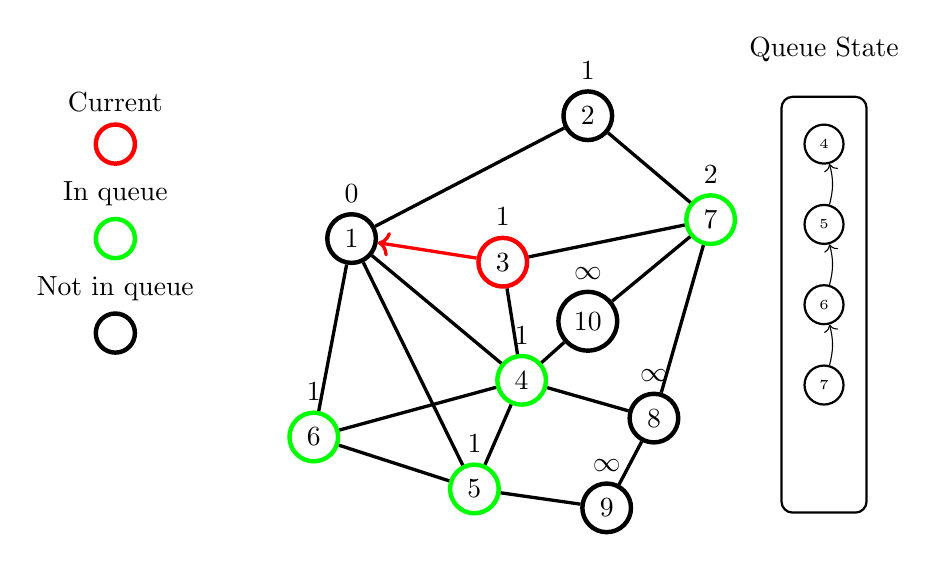
\begin{tikzpicture}[scale=1.2] 
\node[shape=circle, draw=red, 	ultra thick, scale=1.5pt, label={Current}] (U) at (-2.5, 1) {}; 
\node[shape=circle, draw=green,  ultra thick, scale=1.5pt, label={In queue}] (U) at (-2.5, 0) {}; 
\node[shape=circle, draw=black, ultra thick, scale=1.5pt, label={Not in queue}] (U) at (-2.5, -1) {}; 
\draw[thick, rounded corners,draw=black] (4.55, 1.5) rectangle ++(0.9, -1-4*0.85 );
\node[draw=white] at (5, 2) {Queue State} ; 
\node[shape=circle, draw=black, thick, minimum size=2pt] (U0) at (5, 1.0) {\tiny{4}}; 
\node[shape=circle, draw=black, thick, minimum size=2pt] (U1) at (5, 0.15000000000000002) {\tiny{5}}; 
\node[shape=circle, draw=black, thick, minimum size=2pt] (U2) at (5, -0.7) {\tiny{6}}; 
\node[shape=circle, draw=black, thick, minimum size=2pt] (U3) at (5, -1.5499999999999998) {\tiny{7}}; 
\path[->] (U1) edge [out=75, in=-75] (U0);
\path[->] (U2) edge [out=75, in=-75] (U1);
\path[->] (U3) edge [out=75, in=-75] (U2);
\node[shape=circle,draw=black, ultra thick, label={$0$}] (1) at (0,0) {1}; 
\node[shape=circle,draw=black, ultra thick, label={$1$}] (2) at (2.5,1.3) {2}; 
\node[shape=circle,draw=red, ultra thick, label={$1$}] (3) at (1.6,-0.25) {3}; 
\node[shape=circle,draw=green, ultra thick, label={$1$}] (4) at (1.8,-1.5) {4}; 
\node[shape=circle,draw=green, ultra thick, label={$1$}] (5) at (1.3,-2.65) {5}; 
\node[shape=circle,draw=green, ultra thick, label={$1$}] (6) at (-0.4,-2.1) {6}; 
\node[shape=circle,draw=green, ultra thick, label={$2$}] (7) at (3.8,0.2) {7}; 
\node[shape=circle,draw=black, ultra thick, label={$\infty$}] (8) at (3.2,-1.9) {8}; 
\node[shape=circle,draw=black, ultra thick, label={$\infty$}] (9) at (2.7,-2.85) {9}; 
\node[shape=circle,draw=black, ultra thick, label={$\infty$}] (10) at (2.5,-0.875) {10}; 
\path [-,very thick, draw=black] (1) edge  (2);
\path [->,very thick, draw=red] (3) edge  (1);
\path [-,very thick, draw=black] (1) edge  (4);
\path [-,very thick, draw=black] (1) edge  (5);
\path [-,very thick, draw=black] (1) edge  (6);
\path [-,very thick, draw=black] (2) edge  (7);
\path [-,very thick, draw=black] (3) edge  (7);
\path [-,very thick, draw=black] (3) edge  (4);
\path [-,very thick, draw=black] (4) edge  (5);
\path [-,very thick, draw=black] (4) edge  (6);
\path [-,very thick, draw=black] (4) edge  (8);
\path [-,very thick, draw=black] (4) edge  (10);
\path [-,very thick, draw=black] (5) edge  (6);
\path [-,very thick, draw=black] (5) edge  (9);
\path [-,very thick, draw=black] (7) edge  (8);
\path [-,very thick, draw=black] (7) edge  (10);
\path [-,very thick, draw=black] (8) edge  (9);
\end{tikzpicture} 
\end{figure} 
\end{frame} 
\begin{frame}{BFS : Example}
\begin{figure}
\vspace*{-1cm} 
\center
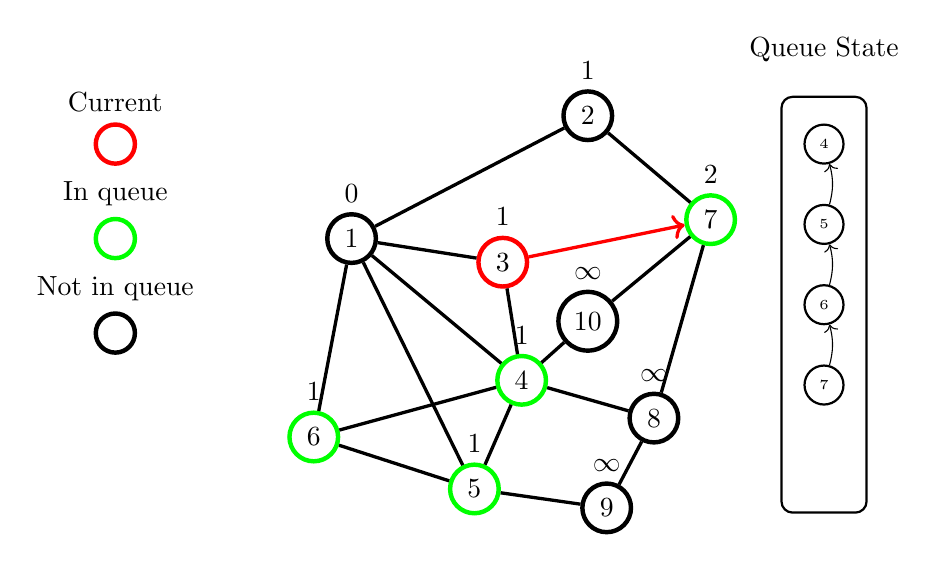
\begin{tikzpicture}[scale=1.2] 
\node[shape=circle, draw=red, 	ultra thick, scale=1.5pt, label={Current}] (U) at (-2.5, 1) {}; 
\node[shape=circle, draw=green,  ultra thick, scale=1.5pt, label={In queue}] (U) at (-2.5, 0) {}; 
\node[shape=circle, draw=black, ultra thick, scale=1.5pt, label={Not in queue}] (U) at (-2.5, -1) {}; 
\draw[thick, rounded corners,draw=black] (4.55, 1.5) rectangle ++(0.9, -1-4*0.85 );
\node[draw=white] at (5, 2) {Queue State} ; 
\node[shape=circle, draw=black, thick, minimum size=2pt] (U0) at (5, 1.0) {\tiny{4}}; 
\node[shape=circle, draw=black, thick, minimum size=2pt] (U1) at (5, 0.15000000000000002) {\tiny{5}}; 
\node[shape=circle, draw=black, thick, minimum size=2pt] (U2) at (5, -0.7) {\tiny{6}}; 
\node[shape=circle, draw=black, thick, minimum size=2pt] (U3) at (5, -1.5499999999999998) {\tiny{7}}; 
\path[->] (U1) edge [out=75, in=-75] (U0);
\path[->] (U2) edge [out=75, in=-75] (U1);
\path[->] (U3) edge [out=75, in=-75] (U2);
\node[shape=circle,draw=black, ultra thick, label={$0$}] (1) at (0,0) {1}; 
\node[shape=circle,draw=black, ultra thick, label={$1$}] (2) at (2.5,1.3) {2}; 
\node[shape=circle,draw=red, ultra thick, label={$1$}] (3) at (1.6,-0.25) {3}; 
\node[shape=circle,draw=green, ultra thick, label={$1$}] (4) at (1.8,-1.5) {4}; 
\node[shape=circle,draw=green, ultra thick, label={$1$}] (5) at (1.3,-2.65) {5}; 
\node[shape=circle,draw=green, ultra thick, label={$1$}] (6) at (-0.4,-2.1) {6}; 
\node[shape=circle,draw=green, ultra thick, label={$2$}] (7) at (3.8,0.2) {7}; 
\node[shape=circle,draw=black, ultra thick, label={$\infty$}] (8) at (3.2,-1.9) {8}; 
\node[shape=circle,draw=black, ultra thick, label={$\infty$}] (9) at (2.7,-2.85) {9}; 
\node[shape=circle,draw=black, ultra thick, label={$\infty$}] (10) at (2.5,-0.875) {10}; 
\path [-,very thick, draw=black] (1) edge  (2);
\path [-,very thick, draw=black] (1) edge  (3);
\path [-,very thick, draw=black] (1) edge  (4);
\path [-,very thick, draw=black] (1) edge  (5);
\path [-,very thick, draw=black] (1) edge  (6);
\path [-,very thick, draw=black] (2) edge  (7);
\path [->,very thick, draw=red] (3) edge  (7);
\path [-,very thick, draw=black] (3) edge  (4);
\path [-,very thick, draw=black] (4) edge  (5);
\path [-,very thick, draw=black] (4) edge  (6);
\path [-,very thick, draw=black] (4) edge  (8);
\path [-,very thick, draw=black] (4) edge  (10);
\path [-,very thick, draw=black] (5) edge  (6);
\path [-,very thick, draw=black] (5) edge  (9);
\path [-,very thick, draw=black] (7) edge  (8);
\path [-,very thick, draw=black] (7) edge  (10);
\path [-,very thick, draw=black] (8) edge  (9);
\end{tikzpicture} 
\end{figure} 
\end{frame} 
\begin{frame}{BFS : Example}
\begin{figure}
\vspace*{-1cm} 
\center
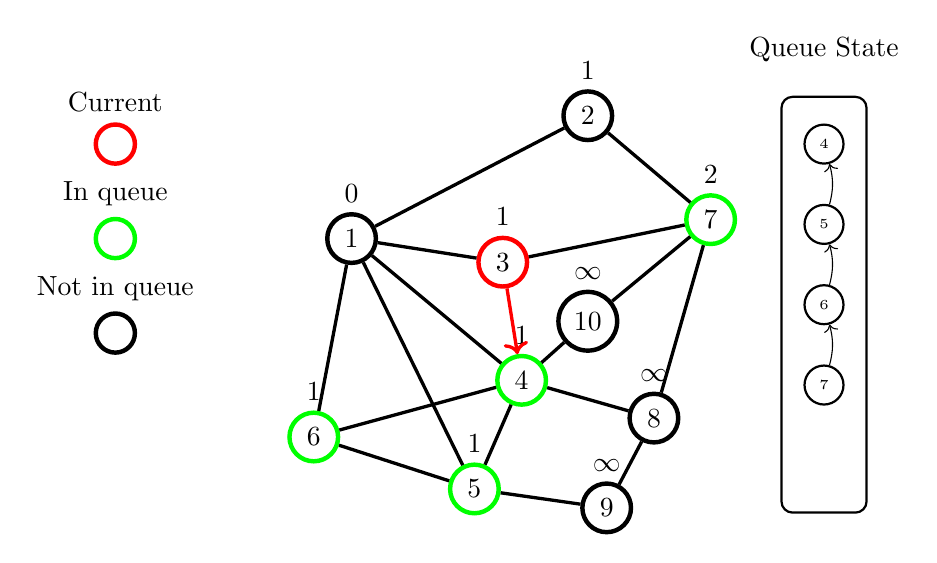
\begin{tikzpicture}[scale=1.2] 
\node[shape=circle, draw=red, 	ultra thick, scale=1.5pt, label={Current}] (U) at (-2.5, 1) {}; 
\node[shape=circle, draw=green,  ultra thick, scale=1.5pt, label={In queue}] (U) at (-2.5, 0) {}; 
\node[shape=circle, draw=black, ultra thick, scale=1.5pt, label={Not in queue}] (U) at (-2.5, -1) {}; 
\draw[thick, rounded corners,draw=black] (4.55, 1.5) rectangle ++(0.9, -1-4*0.85 );
\node[draw=white] at (5, 2) {Queue State} ; 
\node[shape=circle, draw=black, thick, minimum size=2pt] (U0) at (5, 1.0) {\tiny{4}}; 
\node[shape=circle, draw=black, thick, minimum size=2pt] (U1) at (5, 0.15000000000000002) {\tiny{5}}; 
\node[shape=circle, draw=black, thick, minimum size=2pt] (U2) at (5, -0.7) {\tiny{6}}; 
\node[shape=circle, draw=black, thick, minimum size=2pt] (U3) at (5, -1.5499999999999998) {\tiny{7}}; 
\path[->] (U1) edge [out=75, in=-75] (U0);
\path[->] (U2) edge [out=75, in=-75] (U1);
\path[->] (U3) edge [out=75, in=-75] (U2);
\node[shape=circle,draw=black, ultra thick, label={$0$}] (1) at (0,0) {1}; 
\node[shape=circle,draw=black, ultra thick, label={$1$}] (2) at (2.5,1.3) {2}; 
\node[shape=circle,draw=red, ultra thick, label={$1$}] (3) at (1.6,-0.25) {3}; 
\node[shape=circle,draw=green, ultra thick, label={$1$}] (4) at (1.8,-1.5) {4}; 
\node[shape=circle,draw=green, ultra thick, label={$1$}] (5) at (1.3,-2.65) {5}; 
\node[shape=circle,draw=green, ultra thick, label={$1$}] (6) at (-0.4,-2.1) {6}; 
\node[shape=circle,draw=green, ultra thick, label={$2$}] (7) at (3.8,0.2) {7}; 
\node[shape=circle,draw=black, ultra thick, label={$\infty$}] (8) at (3.2,-1.9) {8}; 
\node[shape=circle,draw=black, ultra thick, label={$\infty$}] (9) at (2.7,-2.85) {9}; 
\node[shape=circle,draw=black, ultra thick, label={$\infty$}] (10) at (2.5,-0.875) {10}; 
\path [-,very thick, draw=black] (1) edge  (2);
\path [-,very thick, draw=black] (1) edge  (3);
\path [-,very thick, draw=black] (1) edge  (4);
\path [-,very thick, draw=black] (1) edge  (5);
\path [-,very thick, draw=black] (1) edge  (6);
\path [-,very thick, draw=black] (2) edge  (7);
\path [-,very thick, draw=black] (3) edge  (7);
\path [->,very thick, draw=red] (3) edge  (4);
\path [-,very thick, draw=black] (4) edge  (5);
\path [-,very thick, draw=black] (4) edge  (6);
\path [-,very thick, draw=black] (4) edge  (8);
\path [-,very thick, draw=black] (4) edge  (10);
\path [-,very thick, draw=black] (5) edge  (6);
\path [-,very thick, draw=black] (5) edge  (9);
\path [-,very thick, draw=black] (7) edge  (8);
\path [-,very thick, draw=black] (7) edge  (10);
\path [-,very thick, draw=black] (8) edge  (9);
\end{tikzpicture} 
\end{figure} 
\end{frame} 
\begin{frame}{BFS : Example}
\begin{figure}
\vspace*{-1cm} 
\center
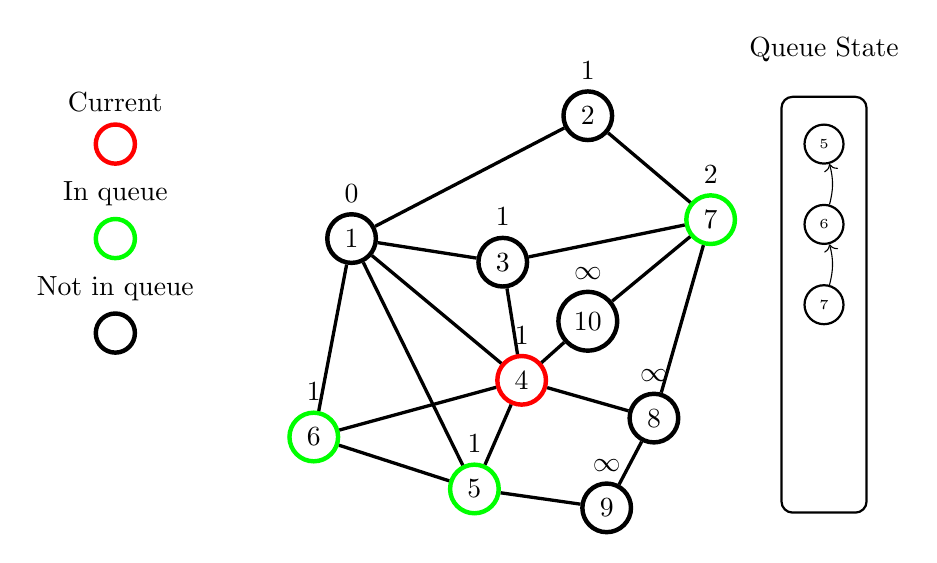
\begin{tikzpicture}[scale=1.2] 
\node[shape=circle, draw=red, 	ultra thick, scale=1.5pt, label={Current}] (U) at (-2.5, 1) {}; 
\node[shape=circle, draw=green,  ultra thick, scale=1.5pt, label={In queue}] (U) at (-2.5, 0) {}; 
\node[shape=circle, draw=black, ultra thick, scale=1.5pt, label={Not in queue}] (U) at (-2.5, -1) {}; 
\draw[thick, rounded corners,draw=black] (4.55, 1.5) rectangle ++(0.9, -1-4*0.85 );
\node[draw=white] at (5, 2) {Queue State} ; 
\node[shape=circle, draw=black, thick, minimum size=2pt] (U0) at (5, 1.0) {\tiny{5}}; 
\node[shape=circle, draw=black, thick, minimum size=2pt] (U1) at (5, 0.15000000000000002) {\tiny{6}}; 
\node[shape=circle, draw=black, thick, minimum size=2pt] (U2) at (5, -0.7) {\tiny{7}}; 
\path[->] (U1) edge [out=75, in=-75] (U0);
\path[->] (U2) edge [out=75, in=-75] (U1);
\node[shape=circle,draw=black, ultra thick, label={$0$}] (1) at (0,0) {1}; 
\node[shape=circle,draw=black, ultra thick, label={$1$}] (2) at (2.5,1.3) {2}; 
\node[shape=circle,draw=black, ultra thick, label={$1$}] (3) at (1.6,-0.25) {3}; 
\node[shape=circle,draw=red, ultra thick, label={$1$}] (4) at (1.8,-1.5) {4}; 
\node[shape=circle,draw=green, ultra thick, label={$1$}] (5) at (1.3,-2.65) {5}; 
\node[shape=circle,draw=green, ultra thick, label={$1$}] (6) at (-0.4,-2.1) {6}; 
\node[shape=circle,draw=green, ultra thick, label={$2$}] (7) at (3.8,0.2) {7}; 
\node[shape=circle,draw=black, ultra thick, label={$\infty$}] (8) at (3.2,-1.9) {8}; 
\node[shape=circle,draw=black, ultra thick, label={$\infty$}] (9) at (2.7,-2.85) {9}; 
\node[shape=circle,draw=black, ultra thick, label={$\infty$}] (10) at (2.5,-0.875) {10}; 
\path [-,very thick, draw=black] (1) edge  (2);
\path [-,very thick, draw=black] (1) edge  (3);
\path [-,very thick, draw=black] (1) edge  (4);
\path [-,very thick, draw=black] (1) edge  (5);
\path [-,very thick, draw=black] (1) edge  (6);
\path [-,very thick, draw=black] (2) edge  (7);
\path [-,very thick, draw=black] (3) edge  (7);
\path [-,very thick, draw=black] (3) edge  (4);
\path [-,very thick, draw=black] (4) edge  (5);
\path [-,very thick, draw=black] (4) edge  (6);
\path [-,very thick, draw=black] (4) edge  (8);
\path [-,very thick, draw=black] (4) edge  (10);
\path [-,very thick, draw=black] (5) edge  (6);
\path [-,very thick, draw=black] (5) edge  (9);
\path [-,very thick, draw=black] (7) edge  (8);
\path [-,very thick, draw=black] (7) edge  (10);
\path [-,very thick, draw=black] (8) edge  (9);
\end{tikzpicture} 
\end{figure} 
\end{frame} 
\begin{frame}{BFS : Example}
\begin{figure}
\vspace*{-1cm} 
\center
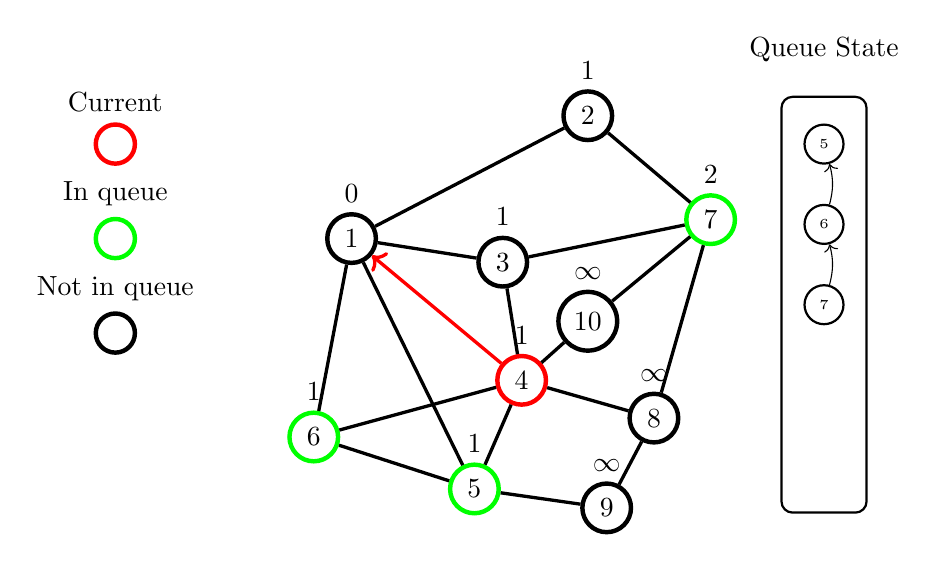
\begin{tikzpicture}[scale=1.2] 
\node[shape=circle, draw=red, 	ultra thick, scale=1.5pt, label={Current}] (U) at (-2.5, 1) {}; 
\node[shape=circle, draw=green,  ultra thick, scale=1.5pt, label={In queue}] (U) at (-2.5, 0) {}; 
\node[shape=circle, draw=black, ultra thick, scale=1.5pt, label={Not in queue}] (U) at (-2.5, -1) {}; 
\draw[thick, rounded corners,draw=black] (4.55, 1.5) rectangle ++(0.9, -1-4*0.85 );
\node[draw=white] at (5, 2) {Queue State} ; 
\node[shape=circle, draw=black, thick, minimum size=2pt] (U0) at (5, 1.0) {\tiny{5}}; 
\node[shape=circle, draw=black, thick, minimum size=2pt] (U1) at (5, 0.15000000000000002) {\tiny{6}}; 
\node[shape=circle, draw=black, thick, minimum size=2pt] (U2) at (5, -0.7) {\tiny{7}}; 
\path[->] (U1) edge [out=75, in=-75] (U0);
\path[->] (U2) edge [out=75, in=-75] (U1);
\node[shape=circle,draw=black, ultra thick, label={$0$}] (1) at (0,0) {1}; 
\node[shape=circle,draw=black, ultra thick, label={$1$}] (2) at (2.5,1.3) {2}; 
\node[shape=circle,draw=black, ultra thick, label={$1$}] (3) at (1.6,-0.25) {3}; 
\node[shape=circle,draw=red, ultra thick, label={$1$}] (4) at (1.8,-1.5) {4}; 
\node[shape=circle,draw=green, ultra thick, label={$1$}] (5) at (1.3,-2.65) {5}; 
\node[shape=circle,draw=green, ultra thick, label={$1$}] (6) at (-0.4,-2.1) {6}; 
\node[shape=circle,draw=green, ultra thick, label={$2$}] (7) at (3.8,0.2) {7}; 
\node[shape=circle,draw=black, ultra thick, label={$\infty$}] (8) at (3.2,-1.9) {8}; 
\node[shape=circle,draw=black, ultra thick, label={$\infty$}] (9) at (2.7,-2.85) {9}; 
\node[shape=circle,draw=black, ultra thick, label={$\infty$}] (10) at (2.5,-0.875) {10}; 
\path [-,very thick, draw=black] (1) edge  (2);
\path [-,very thick, draw=black] (1) edge  (3);
\path [->,very thick, draw=red] (4) edge  (1);
\path [-,very thick, draw=black] (1) edge  (5);
\path [-,very thick, draw=black] (1) edge  (6);
\path [-,very thick, draw=black] (2) edge  (7);
\path [-,very thick, draw=black] (3) edge  (7);
\path [-,very thick, draw=black] (3) edge  (4);
\path [-,very thick, draw=black] (4) edge  (5);
\path [-,very thick, draw=black] (4) edge  (6);
\path [-,very thick, draw=black] (4) edge  (8);
\path [-,very thick, draw=black] (4) edge  (10);
\path [-,very thick, draw=black] (5) edge  (6);
\path [-,very thick, draw=black] (5) edge  (9);
\path [-,very thick, draw=black] (7) edge  (8);
\path [-,very thick, draw=black] (7) edge  (10);
\path [-,very thick, draw=black] (8) edge  (9);
\end{tikzpicture} 
\end{figure} 
\end{frame} 
\begin{frame}{BFS : Example}
\begin{figure}
\vspace*{-1cm} 
\center
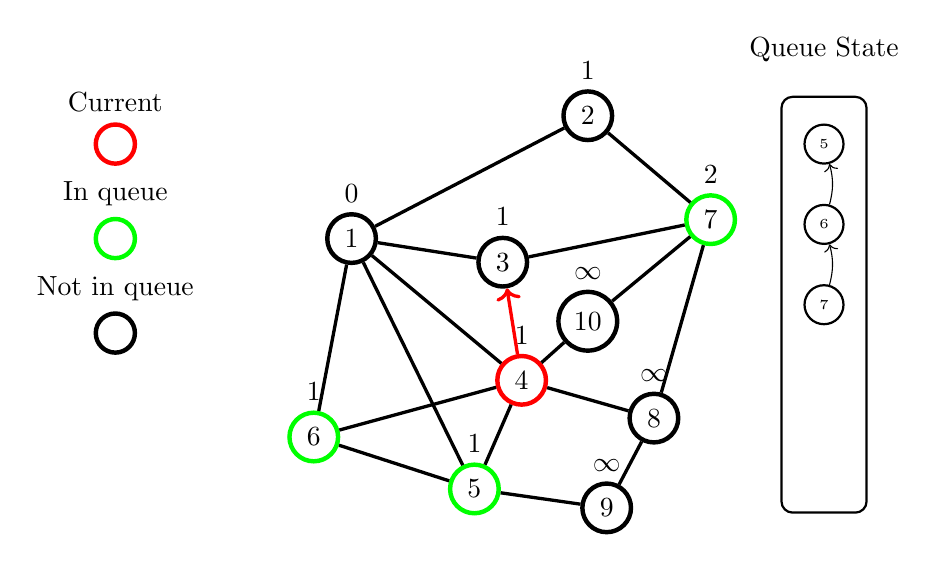
\begin{tikzpicture}[scale=1.2] 
\node[shape=circle, draw=red, 	ultra thick, scale=1.5pt, label={Current}] (U) at (-2.5, 1) {}; 
\node[shape=circle, draw=green,  ultra thick, scale=1.5pt, label={In queue}] (U) at (-2.5, 0) {}; 
\node[shape=circle, draw=black, ultra thick, scale=1.5pt, label={Not in queue}] (U) at (-2.5, -1) {}; 
\draw[thick, rounded corners,draw=black] (4.55, 1.5) rectangle ++(0.9, -1-4*0.85 );
\node[draw=white] at (5, 2) {Queue State} ; 
\node[shape=circle, draw=black, thick, minimum size=2pt] (U0) at (5, 1.0) {\tiny{5}}; 
\node[shape=circle, draw=black, thick, minimum size=2pt] (U1) at (5, 0.15000000000000002) {\tiny{6}}; 
\node[shape=circle, draw=black, thick, minimum size=2pt] (U2) at (5, -0.7) {\tiny{7}}; 
\path[->] (U1) edge [out=75, in=-75] (U0);
\path[->] (U2) edge [out=75, in=-75] (U1);
\node[shape=circle,draw=black, ultra thick, label={$0$}] (1) at (0,0) {1}; 
\node[shape=circle,draw=black, ultra thick, label={$1$}] (2) at (2.5,1.3) {2}; 
\node[shape=circle,draw=black, ultra thick, label={$1$}] (3) at (1.6,-0.25) {3}; 
\node[shape=circle,draw=red, ultra thick, label={$1$}] (4) at (1.8,-1.5) {4}; 
\node[shape=circle,draw=green, ultra thick, label={$1$}] (5) at (1.3,-2.65) {5}; 
\node[shape=circle,draw=green, ultra thick, label={$1$}] (6) at (-0.4,-2.1) {6}; 
\node[shape=circle,draw=green, ultra thick, label={$2$}] (7) at (3.8,0.2) {7}; 
\node[shape=circle,draw=black, ultra thick, label={$\infty$}] (8) at (3.2,-1.9) {8}; 
\node[shape=circle,draw=black, ultra thick, label={$\infty$}] (9) at (2.7,-2.85) {9}; 
\node[shape=circle,draw=black, ultra thick, label={$\infty$}] (10) at (2.5,-0.875) {10}; 
\path [-,very thick, draw=black] (1) edge  (2);
\path [-,very thick, draw=black] (1) edge  (3);
\path [-,very thick, draw=black] (1) edge  (4);
\path [-,very thick, draw=black] (1) edge  (5);
\path [-,very thick, draw=black] (1) edge  (6);
\path [-,very thick, draw=black] (2) edge  (7);
\path [-,very thick, draw=black] (3) edge  (7);
\path [->,very thick, draw=red] (4) edge  (3);
\path [-,very thick, draw=black] (4) edge  (5);
\path [-,very thick, draw=black] (4) edge  (6);
\path [-,very thick, draw=black] (4) edge  (8);
\path [-,very thick, draw=black] (4) edge  (10);
\path [-,very thick, draw=black] (5) edge  (6);
\path [-,very thick, draw=black] (5) edge  (9);
\path [-,very thick, draw=black] (7) edge  (8);
\path [-,very thick, draw=black] (7) edge  (10);
\path [-,very thick, draw=black] (8) edge  (9);
\end{tikzpicture} 
\end{figure} 
\end{frame} 
\begin{frame}{BFS : Example}
\begin{figure}
\vspace*{-1cm} 
\center
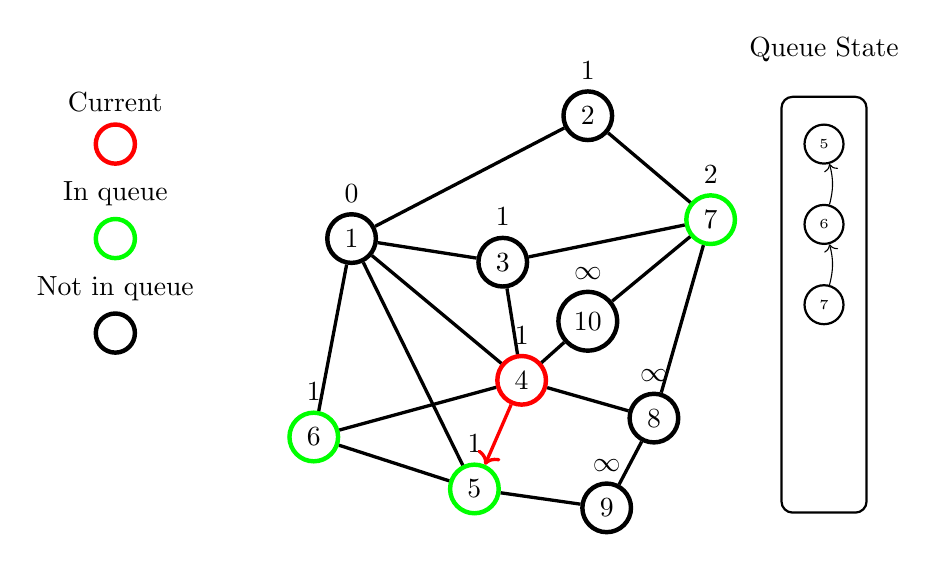
\begin{tikzpicture}[scale=1.2] 
\node[shape=circle, draw=red, 	ultra thick, scale=1.5pt, label={Current}] (U) at (-2.5, 1) {}; 
\node[shape=circle, draw=green,  ultra thick, scale=1.5pt, label={In queue}] (U) at (-2.5, 0) {}; 
\node[shape=circle, draw=black, ultra thick, scale=1.5pt, label={Not in queue}] (U) at (-2.5, -1) {}; 
\draw[thick, rounded corners,draw=black] (4.55, 1.5) rectangle ++(0.9, -1-4*0.85 );
\node[draw=white] at (5, 2) {Queue State} ; 
\node[shape=circle, draw=black, thick, minimum size=2pt] (U0) at (5, 1.0) {\tiny{5}}; 
\node[shape=circle, draw=black, thick, minimum size=2pt] (U1) at (5, 0.15000000000000002) {\tiny{6}}; 
\node[shape=circle, draw=black, thick, minimum size=2pt] (U2) at (5, -0.7) {\tiny{7}}; 
\path[->] (U1) edge [out=75, in=-75] (U0);
\path[->] (U2) edge [out=75, in=-75] (U1);
\node[shape=circle,draw=black, ultra thick, label={$0$}] (1) at (0,0) {1}; 
\node[shape=circle,draw=black, ultra thick, label={$1$}] (2) at (2.5,1.3) {2}; 
\node[shape=circle,draw=black, ultra thick, label={$1$}] (3) at (1.6,-0.25) {3}; 
\node[shape=circle,draw=red, ultra thick, label={$1$}] (4) at (1.8,-1.5) {4}; 
\node[shape=circle,draw=green, ultra thick, label={$1$}] (5) at (1.3,-2.65) {5}; 
\node[shape=circle,draw=green, ultra thick, label={$1$}] (6) at (-0.4,-2.1) {6}; 
\node[shape=circle,draw=green, ultra thick, label={$2$}] (7) at (3.8,0.2) {7}; 
\node[shape=circle,draw=black, ultra thick, label={$\infty$}] (8) at (3.2,-1.9) {8}; 
\node[shape=circle,draw=black, ultra thick, label={$\infty$}] (9) at (2.7,-2.85) {9}; 
\node[shape=circle,draw=black, ultra thick, label={$\infty$}] (10) at (2.5,-0.875) {10}; 
\path [-,very thick, draw=black] (1) edge  (2);
\path [-,very thick, draw=black] (1) edge  (3);
\path [-,very thick, draw=black] (1) edge  (4);
\path [-,very thick, draw=black] (1) edge  (5);
\path [-,very thick, draw=black] (1) edge  (6);
\path [-,very thick, draw=black] (2) edge  (7);
\path [-,very thick, draw=black] (3) edge  (7);
\path [-,very thick, draw=black] (3) edge  (4);
\path [->,very thick, draw=red] (4) edge  (5);
\path [-,very thick, draw=black] (4) edge  (6);
\path [-,very thick, draw=black] (4) edge  (8);
\path [-,very thick, draw=black] (4) edge  (10);
\path [-,very thick, draw=black] (5) edge  (6);
\path [-,very thick, draw=black] (5) edge  (9);
\path [-,very thick, draw=black] (7) edge  (8);
\path [-,very thick, draw=black] (7) edge  (10);
\path [-,very thick, draw=black] (8) edge  (9);
\end{tikzpicture} 
\end{figure} 
\end{frame} 
\begin{frame}{BFS : Example}
\begin{figure}
\vspace*{-1cm} 
\center
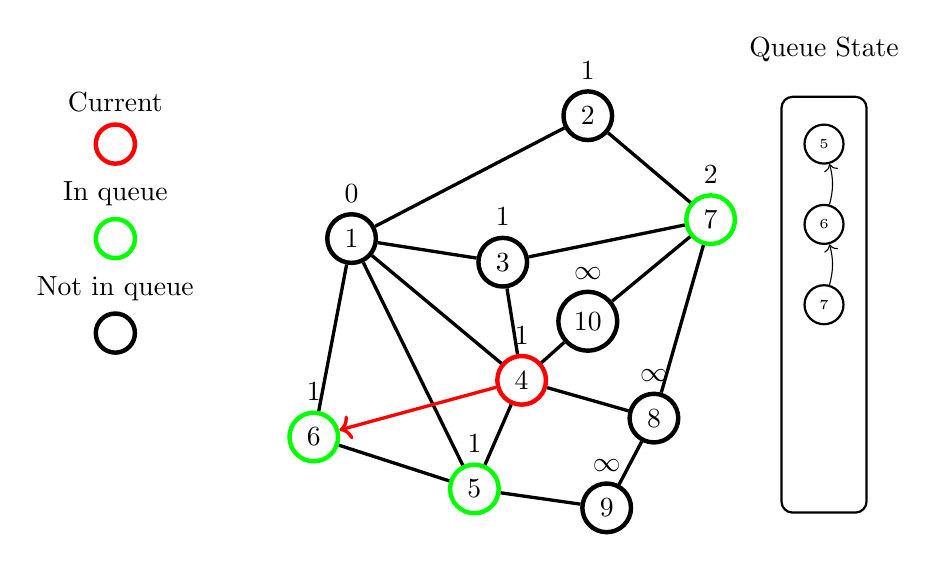
\begin{tikzpicture}[scale=1.2] 
\node[shape=circle, draw=red, 	ultra thick, scale=1.5pt, label={Current}] (U) at (-2.5, 1) {}; 
\node[shape=circle, draw=green,  ultra thick, scale=1.5pt, label={In queue}] (U) at (-2.5, 0) {}; 
\node[shape=circle, draw=black, ultra thick, scale=1.5pt, label={Not in queue}] (U) at (-2.5, -1) {}; 
\draw[thick, rounded corners,draw=black] (4.55, 1.5) rectangle ++(0.9, -1-4*0.85 );
\node[draw=white] at (5, 2) {Queue State} ; 
\node[shape=circle, draw=black, thick, minimum size=2pt] (U0) at (5, 1.0) {\tiny{5}}; 
\node[shape=circle, draw=black, thick, minimum size=2pt] (U1) at (5, 0.15000000000000002) {\tiny{6}}; 
\node[shape=circle, draw=black, thick, minimum size=2pt] (U2) at (5, -0.7) {\tiny{7}}; 
\path[->] (U1) edge [out=75, in=-75] (U0);
\path[->] (U2) edge [out=75, in=-75] (U1);
\node[shape=circle,draw=black, ultra thick, label={$0$}] (1) at (0,0) {1}; 
\node[shape=circle,draw=black, ultra thick, label={$1$}] (2) at (2.5,1.3) {2}; 
\node[shape=circle,draw=black, ultra thick, label={$1$}] (3) at (1.6,-0.25) {3}; 
\node[shape=circle,draw=red, ultra thick, label={$1$}] (4) at (1.8,-1.5) {4}; 
\node[shape=circle,draw=green, ultra thick, label={$1$}] (5) at (1.3,-2.65) {5}; 
\node[shape=circle,draw=green, ultra thick, label={$1$}] (6) at (-0.4,-2.1) {6}; 
\node[shape=circle,draw=green, ultra thick, label={$2$}] (7) at (3.8,0.2) {7}; 
\node[shape=circle,draw=black, ultra thick, label={$\infty$}] (8) at (3.2,-1.9) {8}; 
\node[shape=circle,draw=black, ultra thick, label={$\infty$}] (9) at (2.7,-2.85) {9}; 
\node[shape=circle,draw=black, ultra thick, label={$\infty$}] (10) at (2.5,-0.875) {10}; 
\path [-,very thick, draw=black] (1) edge  (2);
\path [-,very thick, draw=black] (1) edge  (3);
\path [-,very thick, draw=black] (1) edge  (4);
\path [-,very thick, draw=black] (1) edge  (5);
\path [-,very thick, draw=black] (1) edge  (6);
\path [-,very thick, draw=black] (2) edge  (7);
\path [-,very thick, draw=black] (3) edge  (7);
\path [-,very thick, draw=black] (3) edge  (4);
\path [-,very thick, draw=black] (4) edge  (5);
\path [->,very thick, draw=red] (4) edge  (6);
\path [-,very thick, draw=black] (4) edge  (8);
\path [-,very thick, draw=black] (4) edge  (10);
\path [-,very thick, draw=black] (5) edge  (6);
\path [-,very thick, draw=black] (5) edge  (9);
\path [-,very thick, draw=black] (7) edge  (8);
\path [-,very thick, draw=black] (7) edge  (10);
\path [-,very thick, draw=black] (8) edge  (9);
\end{tikzpicture} 
\end{figure} 
\end{frame} 
\begin{frame}{BFS : Example}
\begin{figure}
\vspace*{-1cm} 
\center
\begin{tikzpicture}[scale=1.2] 
\node[shape=circle, draw=red, 	ultra thick, scale=1.5pt, label={Current}] (U) at (-2.5, 1) {}; 
\node[shape=circle, draw=green,  ultra thick, scale=1.5pt, label={In queue}] (U) at (-2.5, 0) {}; 
\node[shape=circle, draw=black, ultra thick, scale=1.5pt, label={Not in queue}] (U) at (-2.5, -1) {}; 
\draw[thick, rounded corners,draw=black] (4.55, 1.5) rectangle ++(0.9, -1-4*0.85 );
\node[draw=white] at (5, 2) {Queue State} ; 
\node[shape=circle, draw=black, thick, minimum size=2pt] (U0) at (5, 1.0) {\tiny{5}}; 
\node[shape=circle, draw=black, thick, minimum size=2pt] (U1) at (5, 0.15000000000000002) {\tiny{6}}; 
\node[shape=circle, draw=black, thick, minimum size=2pt] (U2) at (5, -0.7) {\tiny{7}}; 
\node[shape=circle, draw=black, thick, minimum size=2pt] (U3) at (5, -1.5499999999999998) {\tiny{8}}; 
\path[->] (U1) edge [out=75, in=-75] (U0);
\path[->] (U2) edge [out=75, in=-75] (U1);
\path[->] (U3) edge [out=75, in=-75] (U2);
\path[->, thick, draw=black] (8) edge [dashed, bend right=30] (U3); 
\node[shape=circle,draw=black, ultra thick, label={$0$}] (1) at (0,0) {1}; 
\node[shape=circle,draw=black, ultra thick, label={$1$}] (2) at (2.5,1.3) {2}; 
\node[shape=circle,draw=black, ultra thick, label={$1$}] (3) at (1.6,-0.25) {3}; 
\node[shape=circle,draw=red, ultra thick, label={$1$}] (4) at (1.8,-1.5) {4}; 
\node[shape=circle,draw=green, ultra thick, label={$1$}] (5) at (1.3,-2.65) {5}; 
\node[shape=circle,draw=green, ultra thick, label={$1$}] (6) at (-0.4,-2.1) {6}; 
\node[shape=circle,draw=green, ultra thick, label={$2$}] (7) at (3.8,0.2) {7}; 
\node[shape=circle,draw=green, ultra thick, label={$2$}] (8) at (3.2,-1.9) {8}; 
\node[shape=circle,draw=black, ultra thick, label={$\infty$}] (9) at (2.7,-2.85) {9}; 
\node[shape=circle,draw=black, ultra thick, label={$\infty$}] (10) at (2.5,-0.875) {10}; 
\path [-,very thick, draw=black] (1) edge  (2);
\path [-,very thick, draw=black] (1) edge  (3);
\path [-,very thick, draw=black] (1) edge  (4);
\path [-,very thick, draw=black] (1) edge  (5);
\path [-,very thick, draw=black] (1) edge  (6);
\path [-,very thick, draw=black] (2) edge  (7);
\path [-,very thick, draw=black] (3) edge  (7);
\path [-,very thick, draw=black] (3) edge  (4);
\path [-,very thick, draw=black] (4) edge  (5);
\path [-,very thick, draw=black] (4) edge  (6);
\path [->,very thick, draw=red] (4) edge  (8);
\path [-,very thick, draw=black] (4) edge  (10);
\path [-,very thick, draw=black] (5) edge  (6);
\path [-,very thick, draw=black] (5) edge  (9);
\path [-,very thick, draw=black] (7) edge  (8);
\path [-,very thick, draw=black] (7) edge  (10);
\path [-,very thick, draw=black] (8) edge  (9);
\end{tikzpicture} 
\end{figure} 
\end{frame} 
\begin{frame}{BFS : Example}
\begin{figure}
\vspace*{-1cm} 
\center
\begin{tikzpicture}[scale=1.2] 
\node[shape=circle, draw=red, 	ultra thick, scale=1.5pt, label={Current}] (U) at (-2.5, 1) {}; 
\node[shape=circle, draw=green,  ultra thick, scale=1.5pt, label={In queue}] (U) at (-2.5, 0) {}; 
\node[shape=circle, draw=black, ultra thick, scale=1.5pt, label={Not in queue}] (U) at (-2.5, -1) {}; 
\draw[thick, rounded corners,draw=black] (4.55, 1.5) rectangle ++(0.9, -1-4*0.85 );
\node[draw=white] at (5, 2) {Queue State} ; 
\node[shape=circle, draw=black, thick, minimum size=2pt] (U0) at (5, 1.0) {\tiny{5}}; 
\node[shape=circle, draw=black, thick, minimum size=2pt] (U1) at (5, 0.15000000000000002) {\tiny{6}}; 
\node[shape=circle, draw=black, thick, minimum size=2pt] (U2) at (5, -0.7) {\tiny{7}}; 
\node[shape=circle, draw=black, thick, minimum size=2pt] (U3) at (5, -1.5499999999999998) {\tiny{8}}; 
\node[shape=circle, draw=black, thick, minimum size=2pt] (U4) at (5, -2.4) {\tiny{10}}; 
\path[->] (U1) edge [out=75, in=-75] (U0);
\path[->] (U2) edge [out=75, in=-75] (U1);
\path[->] (U3) edge [out=75, in=-75] (U2);
\path[->] (U4) edge [out=75, in=-75] (U3);
\path[->, thick, draw=black] (10) edge [dashed, bend right=30] (U4); 
\node[shape=circle,draw=black, ultra thick, label={$0$}] (1) at (0,0) {1}; 
\node[shape=circle,draw=black, ultra thick, label={$1$}] (2) at (2.5,1.3) {2}; 
\node[shape=circle,draw=black, ultra thick, label={$1$}] (3) at (1.6,-0.25) {3}; 
\node[shape=circle,draw=red, ultra thick, label={$1$}] (4) at (1.8,-1.5) {4}; 
\node[shape=circle,draw=green, ultra thick, label={$1$}] (5) at (1.3,-2.65) {5}; 
\node[shape=circle,draw=green, ultra thick, label={$1$}] (6) at (-0.4,-2.1) {6}; 
\node[shape=circle,draw=green, ultra thick, label={$2$}] (7) at (3.8,0.2) {7}; 
\node[shape=circle,draw=green, ultra thick, label={$2$}] (8) at (3.2,-1.9) {8}; 
\node[shape=circle,draw=black, ultra thick, label={$\infty$}] (9) at (2.7,-2.85) {9}; 
\node[shape=circle,draw=green, ultra thick, label={$2$}] (10) at (2.5,-0.875) {10}; 
\path [-,very thick, draw=black] (1) edge  (2);
\path [-,very thick, draw=black] (1) edge  (3);
\path [-,very thick, draw=black] (1) edge  (4);
\path [-,very thick, draw=black] (1) edge  (5);
\path [-,very thick, draw=black] (1) edge  (6);
\path [-,very thick, draw=black] (2) edge  (7);
\path [-,very thick, draw=black] (3) edge  (7);
\path [-,very thick, draw=black] (3) edge  (4);
\path [-,very thick, draw=black] (4) edge  (5);
\path [-,very thick, draw=black] (4) edge  (6);
\path [-,very thick, draw=black] (4) edge  (8);
\path [->,very thick, draw=red] (4) edge  (10);
\path [-,very thick, draw=black] (5) edge  (6);
\path [-,very thick, draw=black] (5) edge  (9);
\path [-,very thick, draw=black] (7) edge  (8);
\path [-,very thick, draw=black] (7) edge  (10);
\path [-,very thick, draw=black] (8) edge  (9);
\end{tikzpicture} 
\end{figure} 
\end{frame} 
\begin{frame}{BFS : Example}
\begin{figure}
\vspace*{-1cm} 
\center
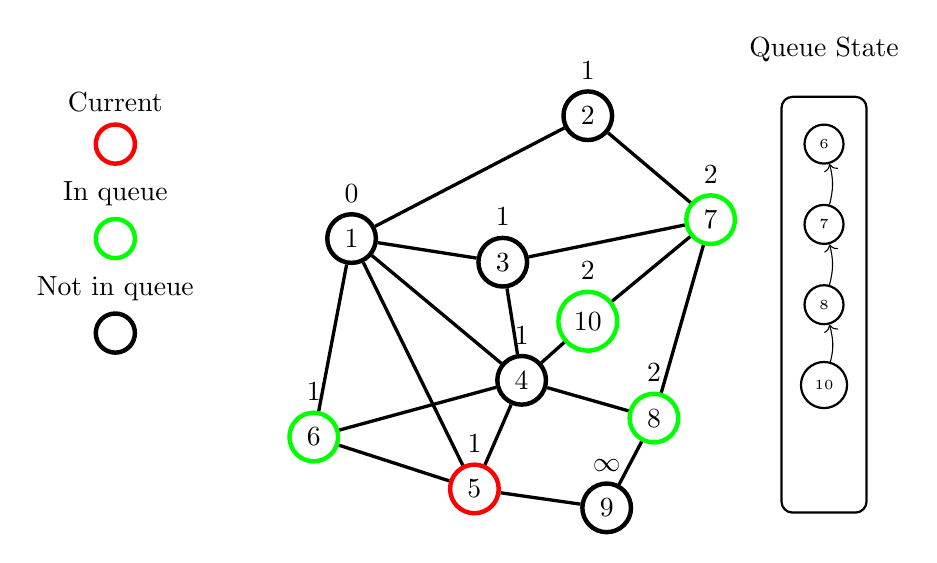
\begin{tikzpicture}[scale=1.2] 
\node[shape=circle, draw=red, 	ultra thick, scale=1.5pt, label={Current}] (U) at (-2.5, 1) {}; 
\node[shape=circle, draw=green,  ultra thick, scale=1.5pt, label={In queue}] (U) at (-2.5, 0) {}; 
\node[shape=circle, draw=black, ultra thick, scale=1.5pt, label={Not in queue}] (U) at (-2.5, -1) {}; 
\draw[thick, rounded corners,draw=black] (4.55, 1.5) rectangle ++(0.9, -1-4*0.85 );
\node[draw=white] at (5, 2) {Queue State} ; 
\node[shape=circle, draw=black, thick, minimum size=2pt] (U0) at (5, 1.0) {\tiny{6}}; 
\node[shape=circle, draw=black, thick, minimum size=2pt] (U1) at (5, 0.15000000000000002) {\tiny{7}}; 
\node[shape=circle, draw=black, thick, minimum size=2pt] (U2) at (5, -0.7) {\tiny{8}}; 
\node[shape=circle, draw=black, thick, minimum size=2pt] (U3) at (5, -1.5499999999999998) {\tiny{10}}; 
\path[->] (U1) edge [out=75, in=-75] (U0);
\path[->] (U2) edge [out=75, in=-75] (U1);
\path[->] (U3) edge [out=75, in=-75] (U2);
\node[shape=circle,draw=black, ultra thick, label={$0$}] (1) at (0,0) {1}; 
\node[shape=circle,draw=black, ultra thick, label={$1$}] (2) at (2.5,1.3) {2}; 
\node[shape=circle,draw=black, ultra thick, label={$1$}] (3) at (1.6,-0.25) {3}; 
\node[shape=circle,draw=black, ultra thick, label={$1$}] (4) at (1.8,-1.5) {4}; 
\node[shape=circle,draw=red, ultra thick, label={$1$}] (5) at (1.3,-2.65) {5}; 
\node[shape=circle,draw=green, ultra thick, label={$1$}] (6) at (-0.4,-2.1) {6}; 
\node[shape=circle,draw=green, ultra thick, label={$2$}] (7) at (3.8,0.2) {7}; 
\node[shape=circle,draw=green, ultra thick, label={$2$}] (8) at (3.2,-1.9) {8}; 
\node[shape=circle,draw=black, ultra thick, label={$\infty$}] (9) at (2.7,-2.85) {9}; 
\node[shape=circle,draw=green, ultra thick, label={$2$}] (10) at (2.5,-0.875) {10}; 
\path [-,very thick, draw=black] (1) edge  (2);
\path [-,very thick, draw=black] (1) edge  (3);
\path [-,very thick, draw=black] (1) edge  (4);
\path [-,very thick, draw=black] (1) edge  (5);
\path [-,very thick, draw=black] (1) edge  (6);
\path [-,very thick, draw=black] (2) edge  (7);
\path [-,very thick, draw=black] (3) edge  (7);
\path [-,very thick, draw=black] (3) edge  (4);
\path [-,very thick, draw=black] (4) edge  (5);
\path [-,very thick, draw=black] (4) edge  (6);
\path [-,very thick, draw=black] (4) edge  (8);
\path [-,very thick, draw=black] (4) edge  (10);
\path [-,very thick, draw=black] (5) edge  (6);
\path [-,very thick, draw=black] (5) edge  (9);
\path [-,very thick, draw=black] (7) edge  (8);
\path [-,very thick, draw=black] (7) edge  (10);
\path [-,very thick, draw=black] (8) edge  (9);
\end{tikzpicture} 
\end{figure} 
\end{frame} 
\begin{frame}{BFS : Example}
\begin{figure}
\vspace*{-1cm} 
\center
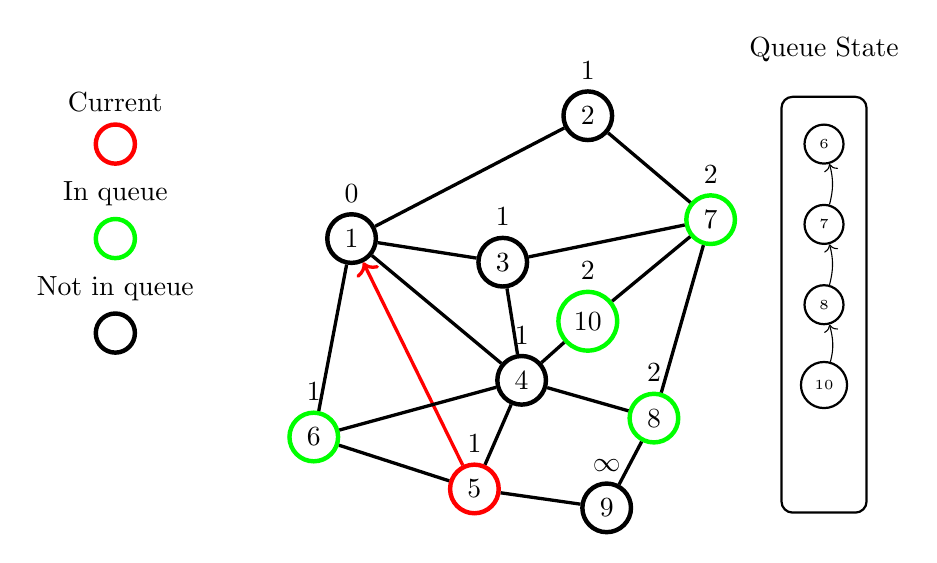
\begin{tikzpicture}[scale=1.2] 
\node[shape=circle, draw=red, 	ultra thick, scale=1.5pt, label={Current}] (U) at (-2.5, 1) {}; 
\node[shape=circle, draw=green,  ultra thick, scale=1.5pt, label={In queue}] (U) at (-2.5, 0) {}; 
\node[shape=circle, draw=black, ultra thick, scale=1.5pt, label={Not in queue}] (U) at (-2.5, -1) {}; 
\draw[thick, rounded corners,draw=black] (4.55, 1.5) rectangle ++(0.9, -1-4*0.85 );
\node[draw=white] at (5, 2) {Queue State} ; 
\node[shape=circle, draw=black, thick, minimum size=2pt] (U0) at (5, 1.0) {\tiny{6}}; 
\node[shape=circle, draw=black, thick, minimum size=2pt] (U1) at (5, 0.15000000000000002) {\tiny{7}}; 
\node[shape=circle, draw=black, thick, minimum size=2pt] (U2) at (5, -0.7) {\tiny{8}}; 
\node[shape=circle, draw=black, thick, minimum size=2pt] (U3) at (5, -1.5499999999999998) {\tiny{10}}; 
\path[->] (U1) edge [out=75, in=-75] (U0);
\path[->] (U2) edge [out=75, in=-75] (U1);
\path[->] (U3) edge [out=75, in=-75] (U2);
\node[shape=circle,draw=black, ultra thick, label={$0$}] (1) at (0,0) {1}; 
\node[shape=circle,draw=black, ultra thick, label={$1$}] (2) at (2.5,1.3) {2}; 
\node[shape=circle,draw=black, ultra thick, label={$1$}] (3) at (1.6,-0.25) {3}; 
\node[shape=circle,draw=black, ultra thick, label={$1$}] (4) at (1.8,-1.5) {4}; 
\node[shape=circle,draw=red, ultra thick, label={$1$}] (5) at (1.3,-2.65) {5}; 
\node[shape=circle,draw=green, ultra thick, label={$1$}] (6) at (-0.4,-2.1) {6}; 
\node[shape=circle,draw=green, ultra thick, label={$2$}] (7) at (3.8,0.2) {7}; 
\node[shape=circle,draw=green, ultra thick, label={$2$}] (8) at (3.2,-1.9) {8}; 
\node[shape=circle,draw=black, ultra thick, label={$\infty$}] (9) at (2.7,-2.85) {9}; 
\node[shape=circle,draw=green, ultra thick, label={$2$}] (10) at (2.5,-0.875) {10}; 
\path [-,very thick, draw=black] (1) edge  (2);
\path [-,very thick, draw=black] (1) edge  (3);
\path [-,very thick, draw=black] (1) edge  (4);
\path [->,very thick, draw=red] (5) edge  (1);
\path [-,very thick, draw=black] (1) edge  (6);
\path [-,very thick, draw=black] (2) edge  (7);
\path [-,very thick, draw=black] (3) edge  (7);
\path [-,very thick, draw=black] (3) edge  (4);
\path [-,very thick, draw=black] (4) edge  (5);
\path [-,very thick, draw=black] (4) edge  (6);
\path [-,very thick, draw=black] (4) edge  (8);
\path [-,very thick, draw=black] (4) edge  (10);
\path [-,very thick, draw=black] (5) edge  (6);
\path [-,very thick, draw=black] (5) edge  (9);
\path [-,very thick, draw=black] (7) edge  (8);
\path [-,very thick, draw=black] (7) edge  (10);
\path [-,very thick, draw=black] (8) edge  (9);
\end{tikzpicture} 
\end{figure} 
\end{frame} 
\begin{frame}{BFS : Example}
\begin{figure}
\vspace*{-1cm} 
\center
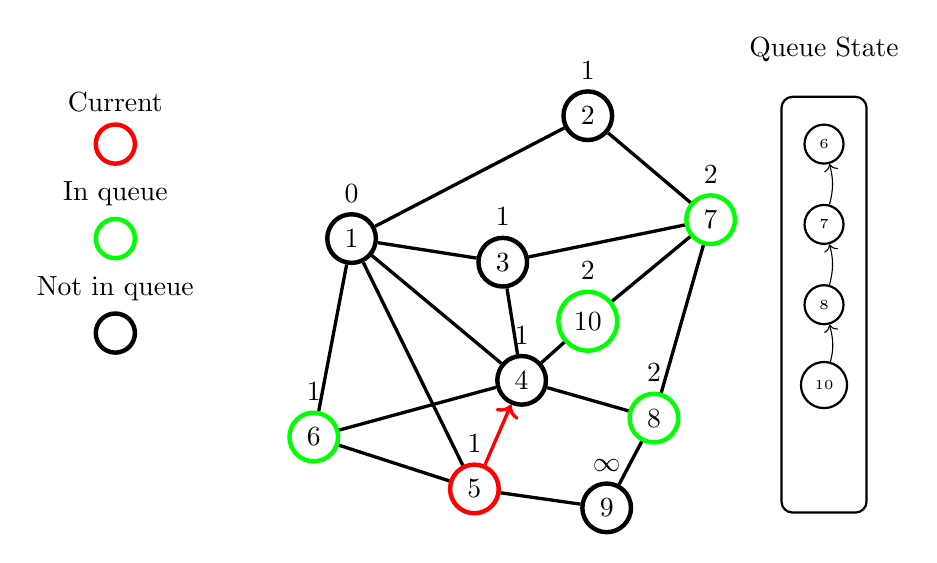
\begin{tikzpicture}[scale=1.2] 
\node[shape=circle, draw=red, 	ultra thick, scale=1.5pt, label={Current}] (U) at (-2.5, 1) {}; 
\node[shape=circle, draw=green,  ultra thick, scale=1.5pt, label={In queue}] (U) at (-2.5, 0) {}; 
\node[shape=circle, draw=black, ultra thick, scale=1.5pt, label={Not in queue}] (U) at (-2.5, -1) {}; 
\draw[thick, rounded corners,draw=black] (4.55, 1.5) rectangle ++(0.9, -1-4*0.85 );
\node[draw=white] at (5, 2) {Queue State} ; 
\node[shape=circle, draw=black, thick, minimum size=2pt] (U0) at (5, 1.0) {\tiny{6}}; 
\node[shape=circle, draw=black, thick, minimum size=2pt] (U1) at (5, 0.15000000000000002) {\tiny{7}}; 
\node[shape=circle, draw=black, thick, minimum size=2pt] (U2) at (5, -0.7) {\tiny{8}}; 
\node[shape=circle, draw=black, thick, minimum size=2pt] (U3) at (5, -1.5499999999999998) {\tiny{10}}; 
\path[->] (U1) edge [out=75, in=-75] (U0);
\path[->] (U2) edge [out=75, in=-75] (U1);
\path[->] (U3) edge [out=75, in=-75] (U2);
\node[shape=circle,draw=black, ultra thick, label={$0$}] (1) at (0,0) {1}; 
\node[shape=circle,draw=black, ultra thick, label={$1$}] (2) at (2.5,1.3) {2}; 
\node[shape=circle,draw=black, ultra thick, label={$1$}] (3) at (1.6,-0.25) {3}; 
\node[shape=circle,draw=black, ultra thick, label={$1$}] (4) at (1.8,-1.5) {4}; 
\node[shape=circle,draw=red, ultra thick, label={$1$}] (5) at (1.3,-2.65) {5}; 
\node[shape=circle,draw=green, ultra thick, label={$1$}] (6) at (-0.4,-2.1) {6}; 
\node[shape=circle,draw=green, ultra thick, label={$2$}] (7) at (3.8,0.2) {7}; 
\node[shape=circle,draw=green, ultra thick, label={$2$}] (8) at (3.2,-1.9) {8}; 
\node[shape=circle,draw=black, ultra thick, label={$\infty$}] (9) at (2.7,-2.85) {9}; 
\node[shape=circle,draw=green, ultra thick, label={$2$}] (10) at (2.5,-0.875) {10}; 
\path [-,very thick, draw=black] (1) edge  (2);
\path [-,very thick, draw=black] (1) edge  (3);
\path [-,very thick, draw=black] (1) edge  (4);
\path [-,very thick, draw=black] (1) edge  (5);
\path [-,very thick, draw=black] (1) edge  (6);
\path [-,very thick, draw=black] (2) edge  (7);
\path [-,very thick, draw=black] (3) edge  (7);
\path [-,very thick, draw=black] (3) edge  (4);
\path [->,very thick, draw=red] (5) edge  (4);
\path [-,very thick, draw=black] (4) edge  (6);
\path [-,very thick, draw=black] (4) edge  (8);
\path [-,very thick, draw=black] (4) edge  (10);
\path [-,very thick, draw=black] (5) edge  (6);
\path [-,very thick, draw=black] (5) edge  (9);
\path [-,very thick, draw=black] (7) edge  (8);
\path [-,very thick, draw=black] (7) edge  (10);
\path [-,very thick, draw=black] (8) edge  (9);
\end{tikzpicture} 
\end{figure} 
\end{frame} 
\begin{frame}{BFS : Example}
\begin{figure}
\vspace*{-1cm} 
\center
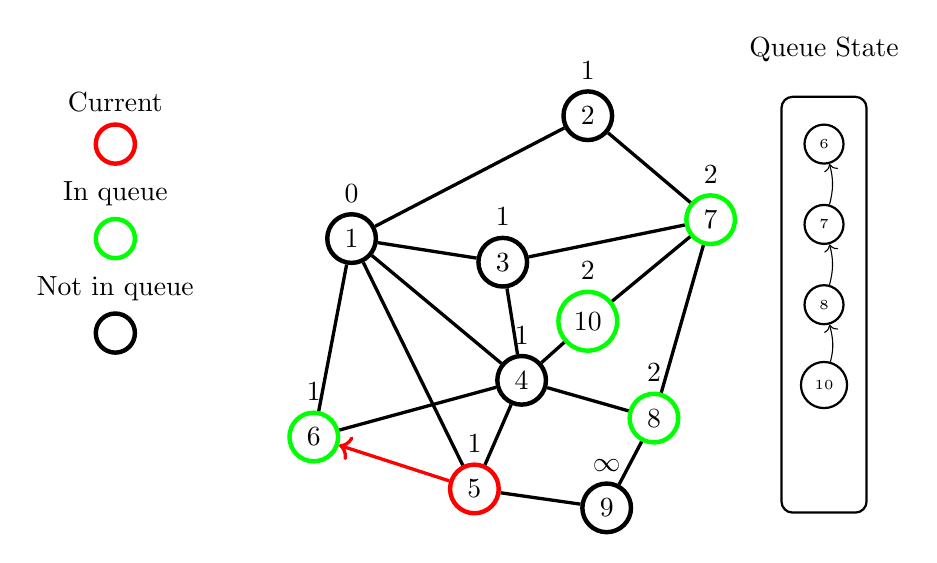
\begin{tikzpicture}[scale=1.2] 
\node[shape=circle, draw=red, 	ultra thick, scale=1.5pt, label={Current}] (U) at (-2.5, 1) {}; 
\node[shape=circle, draw=green,  ultra thick, scale=1.5pt, label={In queue}] (U) at (-2.5, 0) {}; 
\node[shape=circle, draw=black, ultra thick, scale=1.5pt, label={Not in queue}] (U) at (-2.5, -1) {}; 
\draw[thick, rounded corners,draw=black] (4.55, 1.5) rectangle ++(0.9, -1-4*0.85 );
\node[draw=white] at (5, 2) {Queue State} ; 
\node[shape=circle, draw=black, thick, minimum size=2pt] (U0) at (5, 1.0) {\tiny{6}}; 
\node[shape=circle, draw=black, thick, minimum size=2pt] (U1) at (5, 0.15000000000000002) {\tiny{7}}; 
\node[shape=circle, draw=black, thick, minimum size=2pt] (U2) at (5, -0.7) {\tiny{8}}; 
\node[shape=circle, draw=black, thick, minimum size=2pt] (U3) at (5, -1.5499999999999998) {\tiny{10}}; 
\path[->] (U1) edge [out=75, in=-75] (U0);
\path[->] (U2) edge [out=75, in=-75] (U1);
\path[->] (U3) edge [out=75, in=-75] (U2);
\node[shape=circle,draw=black, ultra thick, label={$0$}] (1) at (0,0) {1}; 
\node[shape=circle,draw=black, ultra thick, label={$1$}] (2) at (2.5,1.3) {2}; 
\node[shape=circle,draw=black, ultra thick, label={$1$}] (3) at (1.6,-0.25) {3}; 
\node[shape=circle,draw=black, ultra thick, label={$1$}] (4) at (1.8,-1.5) {4}; 
\node[shape=circle,draw=red, ultra thick, label={$1$}] (5) at (1.3,-2.65) {5}; 
\node[shape=circle,draw=green, ultra thick, label={$1$}] (6) at (-0.4,-2.1) {6}; 
\node[shape=circle,draw=green, ultra thick, label={$2$}] (7) at (3.8,0.2) {7}; 
\node[shape=circle,draw=green, ultra thick, label={$2$}] (8) at (3.2,-1.9) {8}; 
\node[shape=circle,draw=black, ultra thick, label={$\infty$}] (9) at (2.7,-2.85) {9}; 
\node[shape=circle,draw=green, ultra thick, label={$2$}] (10) at (2.5,-0.875) {10}; 
\path [-,very thick, draw=black] (1) edge  (2);
\path [-,very thick, draw=black] (1) edge  (3);
\path [-,very thick, draw=black] (1) edge  (4);
\path [-,very thick, draw=black] (1) edge  (5);
\path [-,very thick, draw=black] (1) edge  (6);
\path [-,very thick, draw=black] (2) edge  (7);
\path [-,very thick, draw=black] (3) edge  (7);
\path [-,very thick, draw=black] (3) edge  (4);
\path [-,very thick, draw=black] (4) edge  (5);
\path [-,very thick, draw=black] (4) edge  (6);
\path [-,very thick, draw=black] (4) edge  (8);
\path [-,very thick, draw=black] (4) edge  (10);
\path [->,very thick, draw=red] (5) edge  (6);
\path [-,very thick, draw=black] (5) edge  (9);
\path [-,very thick, draw=black] (7) edge  (8);
\path [-,very thick, draw=black] (7) edge  (10);
\path [-,very thick, draw=black] (8) edge  (9);
\end{tikzpicture} 
\end{figure} 
\end{frame} 
\begin{frame}{BFS : Example}
\begin{figure}
\vspace*{-1cm} 
\center
\begin{tikzpicture}[scale=1.2] 
\node[shape=circle, draw=red, 	ultra thick, scale=1.5pt, label={Current}] (U) at (-2.5, 1) {}; 
\node[shape=circle, draw=green,  ultra thick, scale=1.5pt, label={In queue}] (U) at (-2.5, 0) {}; 
\node[shape=circle, draw=black, ultra thick, scale=1.5pt, label={Not in queue}] (U) at (-2.5, -1) {}; 
\draw[thick, rounded corners,draw=black] (4.55, 1.5) rectangle ++(0.9, -1-4*0.85 );
\node[draw=white] at (5, 2) {Queue State} ; 
\node[shape=circle, draw=black, thick, minimum size=2pt] (U0) at (5, 1.0) {\tiny{6}}; 
\node[shape=circle, draw=black, thick, minimum size=2pt] (U1) at (5, 0.15000000000000002) {\tiny{7}}; 
\node[shape=circle, draw=black, thick, minimum size=2pt] (U2) at (5, -0.7) {\tiny{8}}; 
\node[shape=circle, draw=black, thick, minimum size=2pt] (U3) at (5, -1.5499999999999998) {\tiny{10}}; 
\node[shape=circle, draw=black, thick, minimum size=2pt] (U4) at (5, -2.4) {\tiny{9}}; 
\path[->] (U1) edge [out=75, in=-75] (U0);
\path[->] (U2) edge [out=75, in=-75] (U1);
\path[->] (U3) edge [out=75, in=-75] (U2);
\path[->] (U4) edge [out=75, in=-75] (U3);
\path[->, thick, draw=black] (9) edge [dashed, bend right=30] (U4); 
\node[shape=circle,draw=black, ultra thick, label={$0$}] (1) at (0,0) {1}; 
\node[shape=circle,draw=black, ultra thick, label={$1$}] (2) at (2.5,1.3) {2}; 
\node[shape=circle,draw=black, ultra thick, label={$1$}] (3) at (1.6,-0.25) {3}; 
\node[shape=circle,draw=black, ultra thick, label={$1$}] (4) at (1.8,-1.5) {4}; 
\node[shape=circle,draw=red, ultra thick, label={$1$}] (5) at (1.3,-2.65) {5}; 
\node[shape=circle,draw=green, ultra thick, label={$1$}] (6) at (-0.4,-2.1) {6}; 
\node[shape=circle,draw=green, ultra thick, label={$2$}] (7) at (3.8,0.2) {7}; 
\node[shape=circle,draw=green, ultra thick, label={$2$}] (8) at (3.2,-1.9) {8}; 
\node[shape=circle,draw=green, ultra thick, label={$2$}] (9) at (2.7,-2.85) {9}; 
\node[shape=circle,draw=green, ultra thick, label={$2$}] (10) at (2.5,-0.875) {10}; 
\path [-,very thick, draw=black] (1) edge  (2);
\path [-,very thick, draw=black] (1) edge  (3);
\path [-,very thick, draw=black] (1) edge  (4);
\path [-,very thick, draw=black] (1) edge  (5);
\path [-,very thick, draw=black] (1) edge  (6);
\path [-,very thick, draw=black] (2) edge  (7);
\path [-,very thick, draw=black] (3) edge  (7);
\path [-,very thick, draw=black] (3) edge  (4);
\path [-,very thick, draw=black] (4) edge  (5);
\path [-,very thick, draw=black] (4) edge  (6);
\path [-,very thick, draw=black] (4) edge  (8);
\path [-,very thick, draw=black] (4) edge  (10);
\path [-,very thick, draw=black] (5) edge  (6);
\path [->,very thick, draw=red] (5) edge  (9);
\path [-,very thick, draw=black] (7) edge  (8);
\path [-,very thick, draw=black] (7) edge  (10);
\path [-,very thick, draw=black] (8) edge  (9);
\end{tikzpicture} 
\end{figure} 
\end{frame} 
\begin{frame}{BFS : Example}
\begin{figure}
\vspace*{-1cm} 
\center
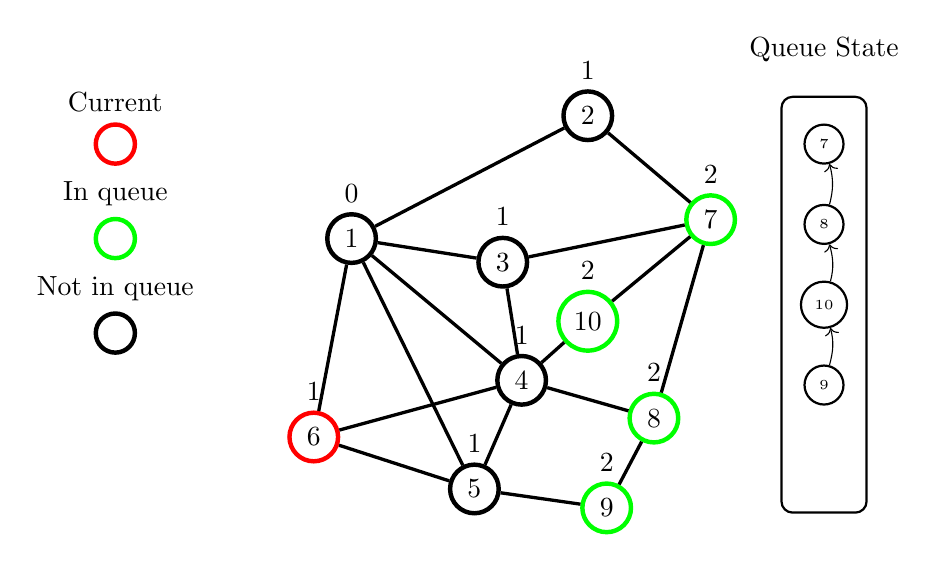
\begin{tikzpicture}[scale=1.2] 
\node[shape=circle, draw=red, 	ultra thick, scale=1.5pt, label={Current}] (U) at (-2.5, 1) {}; 
\node[shape=circle, draw=green,  ultra thick, scale=1.5pt, label={In queue}] (U) at (-2.5, 0) {}; 
\node[shape=circle, draw=black, ultra thick, scale=1.5pt, label={Not in queue}] (U) at (-2.5, -1) {}; 
\draw[thick, rounded corners,draw=black] (4.55, 1.5) rectangle ++(0.9, -1-4*0.85 );
\node[draw=white] at (5, 2) {Queue State} ; 
\node[shape=circle, draw=black, thick, minimum size=2pt] (U0) at (5, 1.0) {\tiny{7}}; 
\node[shape=circle, draw=black, thick, minimum size=2pt] (U1) at (5, 0.15000000000000002) {\tiny{8}}; 
\node[shape=circle, draw=black, thick, minimum size=2pt] (U2) at (5, -0.7) {\tiny{10}}; 
\node[shape=circle, draw=black, thick, minimum size=2pt] (U3) at (5, -1.5499999999999998) {\tiny{9}}; 
\path[->] (U1) edge [out=75, in=-75] (U0);
\path[->] (U2) edge [out=75, in=-75] (U1);
\path[->] (U3) edge [out=75, in=-75] (U2);
\node[shape=circle,draw=black, ultra thick, label={$0$}] (1) at (0,0) {1}; 
\node[shape=circle,draw=black, ultra thick, label={$1$}] (2) at (2.5,1.3) {2}; 
\node[shape=circle,draw=black, ultra thick, label={$1$}] (3) at (1.6,-0.25) {3}; 
\node[shape=circle,draw=black, ultra thick, label={$1$}] (4) at (1.8,-1.5) {4}; 
\node[shape=circle,draw=black, ultra thick, label={$1$}] (5) at (1.3,-2.65) {5}; 
\node[shape=circle,draw=red, ultra thick, label={$1$}] (6) at (-0.4,-2.1) {6}; 
\node[shape=circle,draw=green, ultra thick, label={$2$}] (7) at (3.8,0.2) {7}; 
\node[shape=circle,draw=green, ultra thick, label={$2$}] (8) at (3.2,-1.9) {8}; 
\node[shape=circle,draw=green, ultra thick, label={$2$}] (9) at (2.7,-2.85) {9}; 
\node[shape=circle,draw=green, ultra thick, label={$2$}] (10) at (2.5,-0.875) {10}; 
\path [-,very thick, draw=black] (1) edge  (2);
\path [-,very thick, draw=black] (1) edge  (3);
\path [-,very thick, draw=black] (1) edge  (4);
\path [-,very thick, draw=black] (1) edge  (5);
\path [-,very thick, draw=black] (1) edge  (6);
\path [-,very thick, draw=black] (2) edge  (7);
\path [-,very thick, draw=black] (3) edge  (7);
\path [-,very thick, draw=black] (3) edge  (4);
\path [-,very thick, draw=black] (4) edge  (5);
\path [-,very thick, draw=black] (4) edge  (6);
\path [-,very thick, draw=black] (4) edge  (8);
\path [-,very thick, draw=black] (4) edge  (10);
\path [-,very thick, draw=black] (5) edge  (6);
\path [-,very thick, draw=black] (5) edge  (9);
\path [-,very thick, draw=black] (7) edge  (8);
\path [-,very thick, draw=black] (7) edge  (10);
\path [-,very thick, draw=black] (8) edge  (9);
\end{tikzpicture} 
\end{figure} 
\end{frame} 
\begin{frame}{BFS : Example}
\begin{figure}
\vspace*{-1cm} 
\center
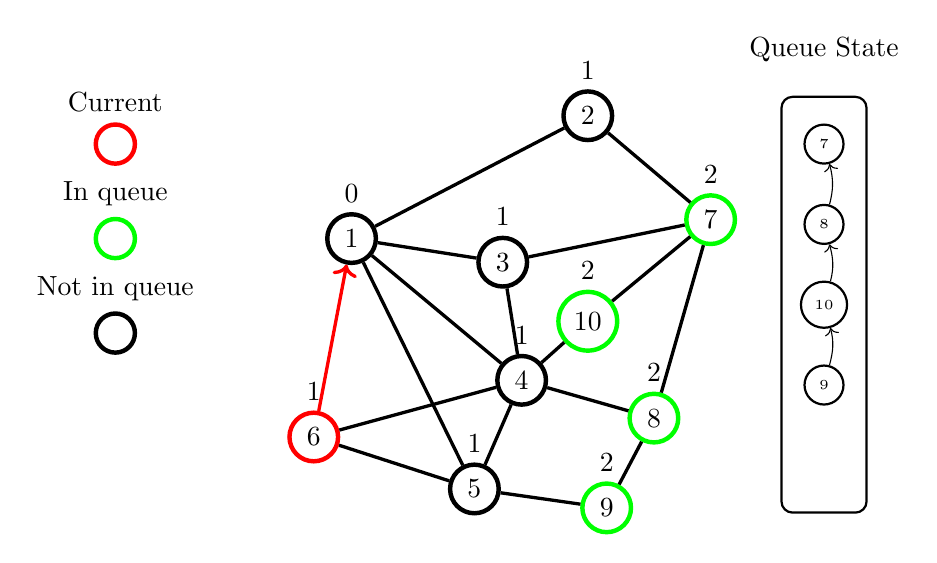
\begin{tikzpicture}[scale=1.2] 
\node[shape=circle, draw=red, 	ultra thick, scale=1.5pt, label={Current}] (U) at (-2.5, 1) {}; 
\node[shape=circle, draw=green,  ultra thick, scale=1.5pt, label={In queue}] (U) at (-2.5, 0) {}; 
\node[shape=circle, draw=black, ultra thick, scale=1.5pt, label={Not in queue}] (U) at (-2.5, -1) {}; 
\draw[thick, rounded corners,draw=black] (4.55, 1.5) rectangle ++(0.9, -1-4*0.85 );
\node[draw=white] at (5, 2) {Queue State} ; 
\node[shape=circle, draw=black, thick, minimum size=2pt] (U0) at (5, 1.0) {\tiny{7}}; 
\node[shape=circle, draw=black, thick, minimum size=2pt] (U1) at (5, 0.15000000000000002) {\tiny{8}}; 
\node[shape=circle, draw=black, thick, minimum size=2pt] (U2) at (5, -0.7) {\tiny{10}}; 
\node[shape=circle, draw=black, thick, minimum size=2pt] (U3) at (5, -1.5499999999999998) {\tiny{9}}; 
\path[->] (U1) edge [out=75, in=-75] (U0);
\path[->] (U2) edge [out=75, in=-75] (U1);
\path[->] (U3) edge [out=75, in=-75] (U2);
\node[shape=circle,draw=black, ultra thick, label={$0$}] (1) at (0,0) {1}; 
\node[shape=circle,draw=black, ultra thick, label={$1$}] (2) at (2.5,1.3) {2}; 
\node[shape=circle,draw=black, ultra thick, label={$1$}] (3) at (1.6,-0.25) {3}; 
\node[shape=circle,draw=black, ultra thick, label={$1$}] (4) at (1.8,-1.5) {4}; 
\node[shape=circle,draw=black, ultra thick, label={$1$}] (5) at (1.3,-2.65) {5}; 
\node[shape=circle,draw=red, ultra thick, label={$1$}] (6) at (-0.4,-2.1) {6}; 
\node[shape=circle,draw=green, ultra thick, label={$2$}] (7) at (3.8,0.2) {7}; 
\node[shape=circle,draw=green, ultra thick, label={$2$}] (8) at (3.2,-1.9) {8}; 
\node[shape=circle,draw=green, ultra thick, label={$2$}] (9) at (2.7,-2.85) {9}; 
\node[shape=circle,draw=green, ultra thick, label={$2$}] (10) at (2.5,-0.875) {10}; 
\path [-,very thick, draw=black] (1) edge  (2);
\path [-,very thick, draw=black] (1) edge  (3);
\path [-,very thick, draw=black] (1) edge  (4);
\path [-,very thick, draw=black] (1) edge  (5);
\path [->,very thick, draw=red] (6) edge  (1);
\path [-,very thick, draw=black] (2) edge  (7);
\path [-,very thick, draw=black] (3) edge  (7);
\path [-,very thick, draw=black] (3) edge  (4);
\path [-,very thick, draw=black] (4) edge  (5);
\path [-,very thick, draw=black] (4) edge  (6);
\path [-,very thick, draw=black] (4) edge  (8);
\path [-,very thick, draw=black] (4) edge  (10);
\path [-,very thick, draw=black] (5) edge  (6);
\path [-,very thick, draw=black] (5) edge  (9);
\path [-,very thick, draw=black] (7) edge  (8);
\path [-,very thick, draw=black] (7) edge  (10);
\path [-,very thick, draw=black] (8) edge  (9);
\end{tikzpicture} 
\end{figure} 
\end{frame} 
\begin{frame}{BFS : Example}
\begin{figure}
\vspace*{-1cm} 
\center
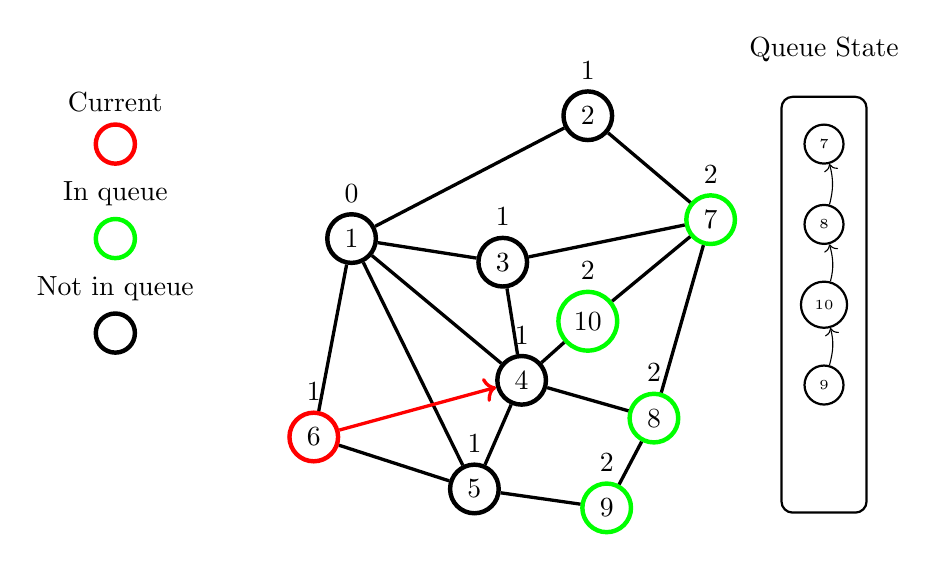
\begin{tikzpicture}[scale=1.2] 
\node[shape=circle, draw=red, 	ultra thick, scale=1.5pt, label={Current}] (U) at (-2.5, 1) {}; 
\node[shape=circle, draw=green,  ultra thick, scale=1.5pt, label={In queue}] (U) at (-2.5, 0) {}; 
\node[shape=circle, draw=black, ultra thick, scale=1.5pt, label={Not in queue}] (U) at (-2.5, -1) {}; 
\draw[thick, rounded corners,draw=black] (4.55, 1.5) rectangle ++(0.9, -1-4*0.85 );
\node[draw=white] at (5, 2) {Queue State} ; 
\node[shape=circle, draw=black, thick, minimum size=2pt] (U0) at (5, 1.0) {\tiny{7}}; 
\node[shape=circle, draw=black, thick, minimum size=2pt] (U1) at (5, 0.15000000000000002) {\tiny{8}}; 
\node[shape=circle, draw=black, thick, minimum size=2pt] (U2) at (5, -0.7) {\tiny{10}}; 
\node[shape=circle, draw=black, thick, minimum size=2pt] (U3) at (5, -1.5499999999999998) {\tiny{9}}; 
\path[->] (U1) edge [out=75, in=-75] (U0);
\path[->] (U2) edge [out=75, in=-75] (U1);
\path[->] (U3) edge [out=75, in=-75] (U2);
\node[shape=circle,draw=black, ultra thick, label={$0$}] (1) at (0,0) {1}; 
\node[shape=circle,draw=black, ultra thick, label={$1$}] (2) at (2.5,1.3) {2}; 
\node[shape=circle,draw=black, ultra thick, label={$1$}] (3) at (1.6,-0.25) {3}; 
\node[shape=circle,draw=black, ultra thick, label={$1$}] (4) at (1.8,-1.5) {4}; 
\node[shape=circle,draw=black, ultra thick, label={$1$}] (5) at (1.3,-2.65) {5}; 
\node[shape=circle,draw=red, ultra thick, label={$1$}] (6) at (-0.4,-2.1) {6}; 
\node[shape=circle,draw=green, ultra thick, label={$2$}] (7) at (3.8,0.2) {7}; 
\node[shape=circle,draw=green, ultra thick, label={$2$}] (8) at (3.2,-1.9) {8}; 
\node[shape=circle,draw=green, ultra thick, label={$2$}] (9) at (2.7,-2.85) {9}; 
\node[shape=circle,draw=green, ultra thick, label={$2$}] (10) at (2.5,-0.875) {10}; 
\path [-,very thick, draw=black] (1) edge  (2);
\path [-,very thick, draw=black] (1) edge  (3);
\path [-,very thick, draw=black] (1) edge  (4);
\path [-,very thick, draw=black] (1) edge  (5);
\path [-,very thick, draw=black] (1) edge  (6);
\path [-,very thick, draw=black] (2) edge  (7);
\path [-,very thick, draw=black] (3) edge  (7);
\path [-,very thick, draw=black] (3) edge  (4);
\path [-,very thick, draw=black] (4) edge  (5);
\path [->,very thick, draw=red] (6) edge  (4);
\path [-,very thick, draw=black] (4) edge  (8);
\path [-,very thick, draw=black] (4) edge  (10);
\path [-,very thick, draw=black] (5) edge  (6);
\path [-,very thick, draw=black] (5) edge  (9);
\path [-,very thick, draw=black] (7) edge  (8);
\path [-,very thick, draw=black] (7) edge  (10);
\path [-,very thick, draw=black] (8) edge  (9);
\end{tikzpicture} 
\end{figure} 
\end{frame} 
\begin{frame}{BFS : Example}
\begin{figure}
\vspace*{-1cm} 
\center
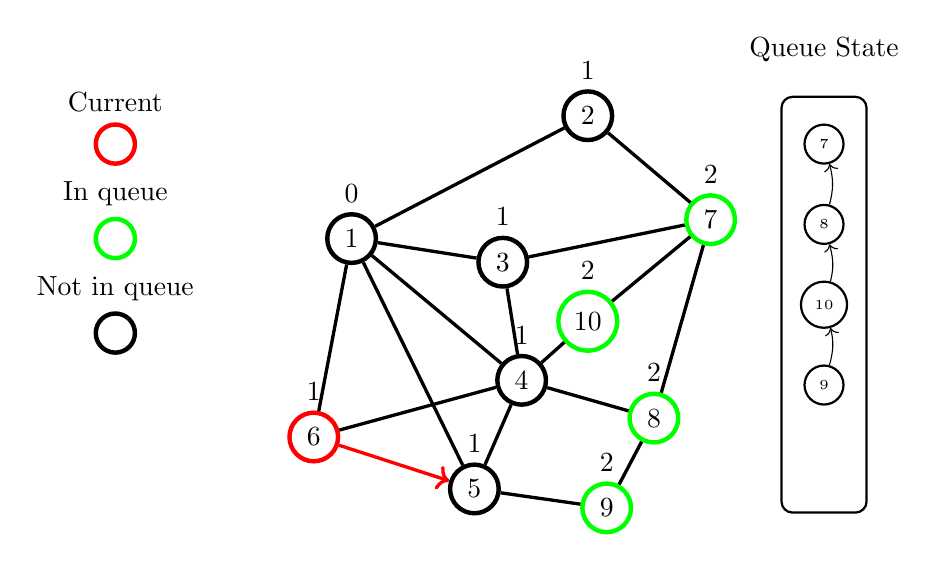
\begin{tikzpicture}[scale=1.2] 
\node[shape=circle, draw=red, 	ultra thick, scale=1.5pt, label={Current}] (U) at (-2.5, 1) {}; 
\node[shape=circle, draw=green,  ultra thick, scale=1.5pt, label={In queue}] (U) at (-2.5, 0) {}; 
\node[shape=circle, draw=black, ultra thick, scale=1.5pt, label={Not in queue}] (U) at (-2.5, -1) {}; 
\draw[thick, rounded corners,draw=black] (4.55, 1.5) rectangle ++(0.9, -1-4*0.85 );
\node[draw=white] at (5, 2) {Queue State} ; 
\node[shape=circle, draw=black, thick, minimum size=2pt] (U0) at (5, 1.0) {\tiny{7}}; 
\node[shape=circle, draw=black, thick, minimum size=2pt] (U1) at (5, 0.15000000000000002) {\tiny{8}}; 
\node[shape=circle, draw=black, thick, minimum size=2pt] (U2) at (5, -0.7) {\tiny{10}}; 
\node[shape=circle, draw=black, thick, minimum size=2pt] (U3) at (5, -1.5499999999999998) {\tiny{9}}; 
\path[->] (U1) edge [out=75, in=-75] (U0);
\path[->] (U2) edge [out=75, in=-75] (U1);
\path[->] (U3) edge [out=75, in=-75] (U2);
\node[shape=circle,draw=black, ultra thick, label={$0$}] (1) at (0,0) {1}; 
\node[shape=circle,draw=black, ultra thick, label={$1$}] (2) at (2.5,1.3) {2}; 
\node[shape=circle,draw=black, ultra thick, label={$1$}] (3) at (1.6,-0.25) {3}; 
\node[shape=circle,draw=black, ultra thick, label={$1$}] (4) at (1.8,-1.5) {4}; 
\node[shape=circle,draw=black, ultra thick, label={$1$}] (5) at (1.3,-2.65) {5}; 
\node[shape=circle,draw=red, ultra thick, label={$1$}] (6) at (-0.4,-2.1) {6}; 
\node[shape=circle,draw=green, ultra thick, label={$2$}] (7) at (3.8,0.2) {7}; 
\node[shape=circle,draw=green, ultra thick, label={$2$}] (8) at (3.2,-1.9) {8}; 
\node[shape=circle,draw=green, ultra thick, label={$2$}] (9) at (2.7,-2.85) {9}; 
\node[shape=circle,draw=green, ultra thick, label={$2$}] (10) at (2.5,-0.875) {10}; 
\path [-,very thick, draw=black] (1) edge  (2);
\path [-,very thick, draw=black] (1) edge  (3);
\path [-,very thick, draw=black] (1) edge  (4);
\path [-,very thick, draw=black] (1) edge  (5);
\path [-,very thick, draw=black] (1) edge  (6);
\path [-,very thick, draw=black] (2) edge  (7);
\path [-,very thick, draw=black] (3) edge  (7);
\path [-,very thick, draw=black] (3) edge  (4);
\path [-,very thick, draw=black] (4) edge  (5);
\path [-,very thick, draw=black] (4) edge  (6);
\path [-,very thick, draw=black] (4) edge  (8);
\path [-,very thick, draw=black] (4) edge  (10);
\path [->,very thick, draw=red] (6) edge  (5);
\path [-,very thick, draw=black] (5) edge  (9);
\path [-,very thick, draw=black] (7) edge  (8);
\path [-,very thick, draw=black] (7) edge  (10);
\path [-,very thick, draw=black] (8) edge  (9);
\end{tikzpicture} 
\end{figure} 
\end{frame} 
\begin{frame}{BFS : Example}
\begin{figure}
\vspace*{-1cm} 
\center
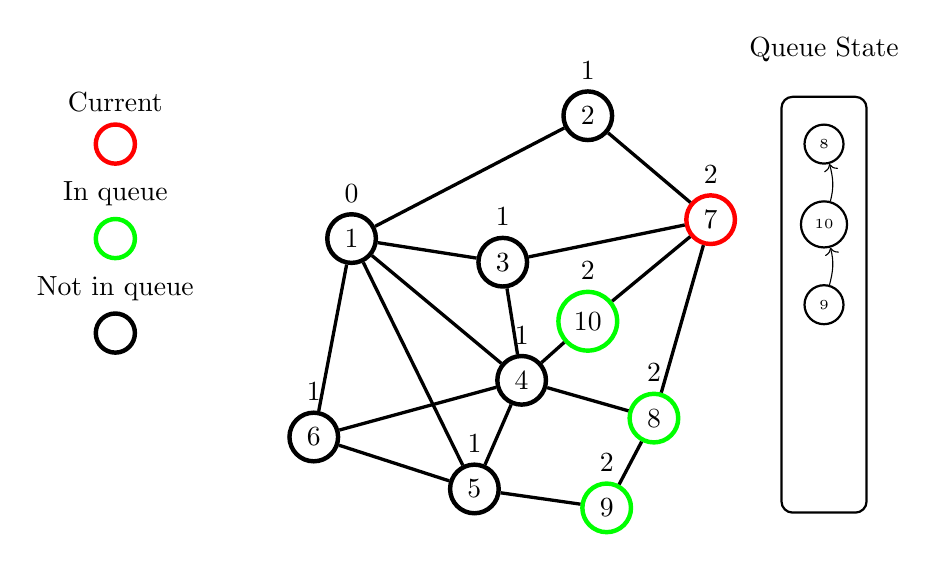
\begin{tikzpicture}[scale=1.2] 
\node[shape=circle, draw=red, 	ultra thick, scale=1.5pt, label={Current}] (U) at (-2.5, 1) {}; 
\node[shape=circle, draw=green,  ultra thick, scale=1.5pt, label={In queue}] (U) at (-2.5, 0) {}; 
\node[shape=circle, draw=black, ultra thick, scale=1.5pt, label={Not in queue}] (U) at (-2.5, -1) {}; 
\draw[thick, rounded corners,draw=black] (4.55, 1.5) rectangle ++(0.9, -1-4*0.85 );
\node[draw=white] at (5, 2) {Queue State} ; 
\node[shape=circle, draw=black, thick, minimum size=2pt] (U0) at (5, 1.0) {\tiny{8}}; 
\node[shape=circle, draw=black, thick, minimum size=2pt] (U1) at (5, 0.15000000000000002) {\tiny{10}}; 
\node[shape=circle, draw=black, thick, minimum size=2pt] (U2) at (5, -0.7) {\tiny{9}}; 
\path[->] (U1) edge [out=75, in=-75] (U0);
\path[->] (U2) edge [out=75, in=-75] (U1);
\node[shape=circle,draw=black, ultra thick, label={$0$}] (1) at (0,0) {1}; 
\node[shape=circle,draw=black, ultra thick, label={$1$}] (2) at (2.5,1.3) {2}; 
\node[shape=circle,draw=black, ultra thick, label={$1$}] (3) at (1.6,-0.25) {3}; 
\node[shape=circle,draw=black, ultra thick, label={$1$}] (4) at (1.8,-1.5) {4}; 
\node[shape=circle,draw=black, ultra thick, label={$1$}] (5) at (1.3,-2.65) {5}; 
\node[shape=circle,draw=black, ultra thick, label={$1$}] (6) at (-0.4,-2.1) {6}; 
\node[shape=circle,draw=red, ultra thick, label={$2$}] (7) at (3.8,0.2) {7}; 
\node[shape=circle,draw=green, ultra thick, label={$2$}] (8) at (3.2,-1.9) {8}; 
\node[shape=circle,draw=green, ultra thick, label={$2$}] (9) at (2.7,-2.85) {9}; 
\node[shape=circle,draw=green, ultra thick, label={$2$}] (10) at (2.5,-0.875) {10}; 
\path [-,very thick, draw=black] (1) edge  (2);
\path [-,very thick, draw=black] (1) edge  (3);
\path [-,very thick, draw=black] (1) edge  (4);
\path [-,very thick, draw=black] (1) edge  (5);
\path [-,very thick, draw=black] (1) edge  (6);
\path [-,very thick, draw=black] (2) edge  (7);
\path [-,very thick, draw=black] (3) edge  (7);
\path [-,very thick, draw=black] (3) edge  (4);
\path [-,very thick, draw=black] (4) edge  (5);
\path [-,very thick, draw=black] (4) edge  (6);
\path [-,very thick, draw=black] (4) edge  (8);
\path [-,very thick, draw=black] (4) edge  (10);
\path [-,very thick, draw=black] (5) edge  (6);
\path [-,very thick, draw=black] (5) edge  (9);
\path [-,very thick, draw=black] (7) edge  (8);
\path [-,very thick, draw=black] (7) edge  (10);
\path [-,very thick, draw=black] (8) edge  (9);
\end{tikzpicture} 
\end{figure} 
\end{frame} 
\begin{frame}{BFS : Example}
\begin{figure}
\vspace*{-1cm} 
\center
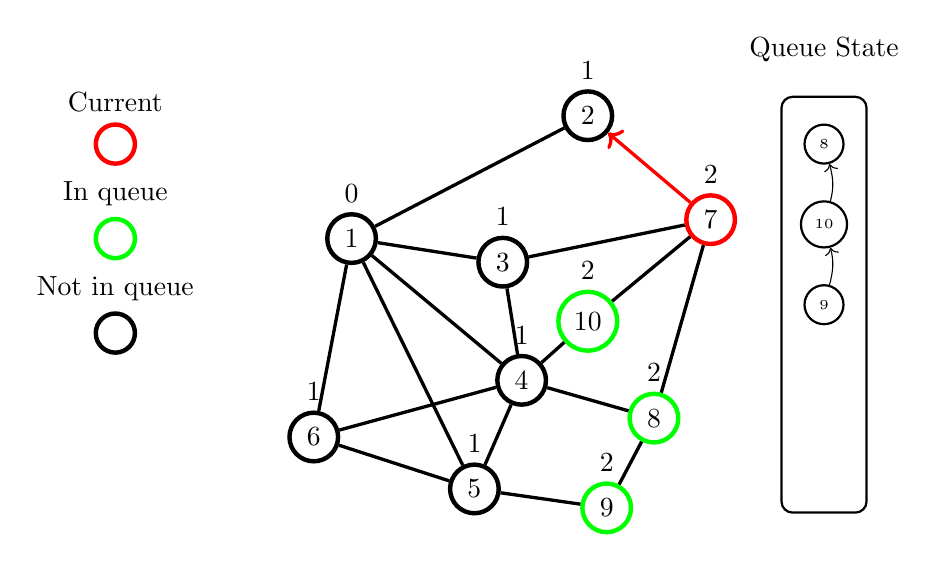
\begin{tikzpicture}[scale=1.2] 
\node[shape=circle, draw=red, 	ultra thick, scale=1.5pt, label={Current}] (U) at (-2.5, 1) {}; 
\node[shape=circle, draw=green,  ultra thick, scale=1.5pt, label={In queue}] (U) at (-2.5, 0) {}; 
\node[shape=circle, draw=black, ultra thick, scale=1.5pt, label={Not in queue}] (U) at (-2.5, -1) {}; 
\draw[thick, rounded corners,draw=black] (4.55, 1.5) rectangle ++(0.9, -1-4*0.85 );
\node[draw=white] at (5, 2) {Queue State} ; 
\node[shape=circle, draw=black, thick, minimum size=2pt] (U0) at (5, 1.0) {\tiny{8}}; 
\node[shape=circle, draw=black, thick, minimum size=2pt] (U1) at (5, 0.15000000000000002) {\tiny{10}}; 
\node[shape=circle, draw=black, thick, minimum size=2pt] (U2) at (5, -0.7) {\tiny{9}}; 
\path[->] (U1) edge [out=75, in=-75] (U0);
\path[->] (U2) edge [out=75, in=-75] (U1);
\node[shape=circle,draw=black, ultra thick, label={$0$}] (1) at (0,0) {1}; 
\node[shape=circle,draw=black, ultra thick, label={$1$}] (2) at (2.5,1.3) {2}; 
\node[shape=circle,draw=black, ultra thick, label={$1$}] (3) at (1.6,-0.25) {3}; 
\node[shape=circle,draw=black, ultra thick, label={$1$}] (4) at (1.8,-1.5) {4}; 
\node[shape=circle,draw=black, ultra thick, label={$1$}] (5) at (1.3,-2.65) {5}; 
\node[shape=circle,draw=black, ultra thick, label={$1$}] (6) at (-0.4,-2.1) {6}; 
\node[shape=circle,draw=red, ultra thick, label={$2$}] (7) at (3.8,0.2) {7}; 
\node[shape=circle,draw=green, ultra thick, label={$2$}] (8) at (3.2,-1.9) {8}; 
\node[shape=circle,draw=green, ultra thick, label={$2$}] (9) at (2.7,-2.85) {9}; 
\node[shape=circle,draw=green, ultra thick, label={$2$}] (10) at (2.5,-0.875) {10}; 
\path [-,very thick, draw=black] (1) edge  (2);
\path [-,very thick, draw=black] (1) edge  (3);
\path [-,very thick, draw=black] (1) edge  (4);
\path [-,very thick, draw=black] (1) edge  (5);
\path [-,very thick, draw=black] (1) edge  (6);
\path [->,very thick, draw=red] (7) edge  (2);
\path [-,very thick, draw=black] (3) edge  (7);
\path [-,very thick, draw=black] (3) edge  (4);
\path [-,very thick, draw=black] (4) edge  (5);
\path [-,very thick, draw=black] (4) edge  (6);
\path [-,very thick, draw=black] (4) edge  (8);
\path [-,very thick, draw=black] (4) edge  (10);
\path [-,very thick, draw=black] (5) edge  (6);
\path [-,very thick, draw=black] (5) edge  (9);
\path [-,very thick, draw=black] (7) edge  (8);
\path [-,very thick, draw=black] (7) edge  (10);
\path [-,very thick, draw=black] (8) edge  (9);
\end{tikzpicture} 
\end{figure} 
\end{frame} 
\begin{frame}{BFS : Example}
\begin{figure}
\vspace*{-1cm} 
\center
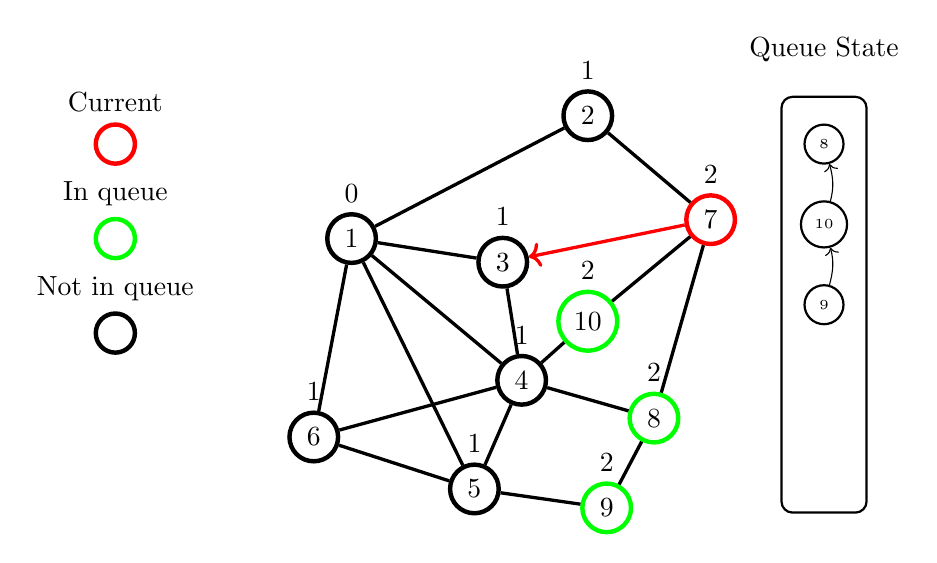
\begin{tikzpicture}[scale=1.2] 
\node[shape=circle, draw=red, 	ultra thick, scale=1.5pt, label={Current}] (U) at (-2.5, 1) {}; 
\node[shape=circle, draw=green,  ultra thick, scale=1.5pt, label={In queue}] (U) at (-2.5, 0) {}; 
\node[shape=circle, draw=black, ultra thick, scale=1.5pt, label={Not in queue}] (U) at (-2.5, -1) {}; 
\draw[thick, rounded corners,draw=black] (4.55, 1.5) rectangle ++(0.9, -1-4*0.85 );
\node[draw=white] at (5, 2) {Queue State} ; 
\node[shape=circle, draw=black, thick, minimum size=2pt] (U0) at (5, 1.0) {\tiny{8}}; 
\node[shape=circle, draw=black, thick, minimum size=2pt] (U1) at (5, 0.15000000000000002) {\tiny{10}}; 
\node[shape=circle, draw=black, thick, minimum size=2pt] (U2) at (5, -0.7) {\tiny{9}}; 
\path[->] (U1) edge [out=75, in=-75] (U0);
\path[->] (U2) edge [out=75, in=-75] (U1);
\node[shape=circle,draw=black, ultra thick, label={$0$}] (1) at (0,0) {1}; 
\node[shape=circle,draw=black, ultra thick, label={$1$}] (2) at (2.5,1.3) {2}; 
\node[shape=circle,draw=black, ultra thick, label={$1$}] (3) at (1.6,-0.25) {3}; 
\node[shape=circle,draw=black, ultra thick, label={$1$}] (4) at (1.8,-1.5) {4}; 
\node[shape=circle,draw=black, ultra thick, label={$1$}] (5) at (1.3,-2.65) {5}; 
\node[shape=circle,draw=black, ultra thick, label={$1$}] (6) at (-0.4,-2.1) {6}; 
\node[shape=circle,draw=red, ultra thick, label={$2$}] (7) at (3.8,0.2) {7}; 
\node[shape=circle,draw=green, ultra thick, label={$2$}] (8) at (3.2,-1.9) {8}; 
\node[shape=circle,draw=green, ultra thick, label={$2$}] (9) at (2.7,-2.85) {9}; 
\node[shape=circle,draw=green, ultra thick, label={$2$}] (10) at (2.5,-0.875) {10}; 
\path [-,very thick, draw=black] (1) edge  (2);
\path [-,very thick, draw=black] (1) edge  (3);
\path [-,very thick, draw=black] (1) edge  (4);
\path [-,very thick, draw=black] (1) edge  (5);
\path [-,very thick, draw=black] (1) edge  (6);
\path [-,very thick, draw=black] (2) edge  (7);
\path [->,very thick, draw=red] (7) edge  (3);
\path [-,very thick, draw=black] (3) edge  (4);
\path [-,very thick, draw=black] (4) edge  (5);
\path [-,very thick, draw=black] (4) edge  (6);
\path [-,very thick, draw=black] (4) edge  (8);
\path [-,very thick, draw=black] (4) edge  (10);
\path [-,very thick, draw=black] (5) edge  (6);
\path [-,very thick, draw=black] (5) edge  (9);
\path [-,very thick, draw=black] (7) edge  (8);
\path [-,very thick, draw=black] (7) edge  (10);
\path [-,very thick, draw=black] (8) edge  (9);
\end{tikzpicture} 
\end{figure} 
\end{frame} 
\begin{frame}{BFS : Example}
\begin{figure}
\vspace*{-1cm} 
\center
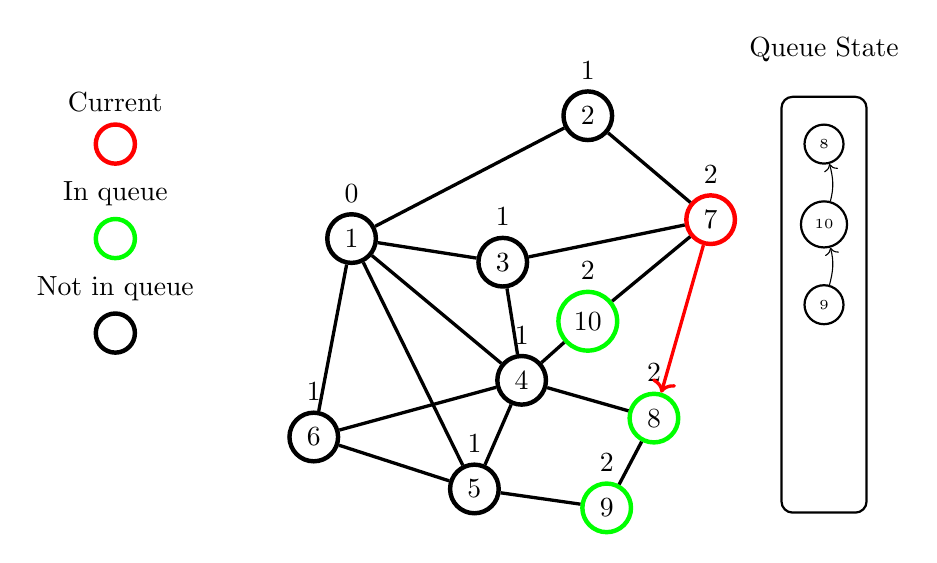
\begin{tikzpicture}[scale=1.2] 
\node[shape=circle, draw=red, 	ultra thick, scale=1.5pt, label={Current}] (U) at (-2.5, 1) {}; 
\node[shape=circle, draw=green,  ultra thick, scale=1.5pt, label={In queue}] (U) at (-2.5, 0) {}; 
\node[shape=circle, draw=black, ultra thick, scale=1.5pt, label={Not in queue}] (U) at (-2.5, -1) {}; 
\draw[thick, rounded corners,draw=black] (4.55, 1.5) rectangle ++(0.9, -1-4*0.85 );
\node[draw=white] at (5, 2) {Queue State} ; 
\node[shape=circle, draw=black, thick, minimum size=2pt] (U0) at (5, 1.0) {\tiny{8}}; 
\node[shape=circle, draw=black, thick, minimum size=2pt] (U1) at (5, 0.15000000000000002) {\tiny{10}}; 
\node[shape=circle, draw=black, thick, minimum size=2pt] (U2) at (5, -0.7) {\tiny{9}}; 
\path[->] (U1) edge [out=75, in=-75] (U0);
\path[->] (U2) edge [out=75, in=-75] (U1);
\node[shape=circle,draw=black, ultra thick, label={$0$}] (1) at (0,0) {1}; 
\node[shape=circle,draw=black, ultra thick, label={$1$}] (2) at (2.5,1.3) {2}; 
\node[shape=circle,draw=black, ultra thick, label={$1$}] (3) at (1.6,-0.25) {3}; 
\node[shape=circle,draw=black, ultra thick, label={$1$}] (4) at (1.8,-1.5) {4}; 
\node[shape=circle,draw=black, ultra thick, label={$1$}] (5) at (1.3,-2.65) {5}; 
\node[shape=circle,draw=black, ultra thick, label={$1$}] (6) at (-0.4,-2.1) {6}; 
\node[shape=circle,draw=red, ultra thick, label={$2$}] (7) at (3.8,0.2) {7}; 
\node[shape=circle,draw=green, ultra thick, label={$2$}] (8) at (3.2,-1.9) {8}; 
\node[shape=circle,draw=green, ultra thick, label={$2$}] (9) at (2.7,-2.85) {9}; 
\node[shape=circle,draw=green, ultra thick, label={$2$}] (10) at (2.5,-0.875) {10}; 
\path [-,very thick, draw=black] (1) edge  (2);
\path [-,very thick, draw=black] (1) edge  (3);
\path [-,very thick, draw=black] (1) edge  (4);
\path [-,very thick, draw=black] (1) edge  (5);
\path [-,very thick, draw=black] (1) edge  (6);
\path [-,very thick, draw=black] (2) edge  (7);
\path [-,very thick, draw=black] (3) edge  (7);
\path [-,very thick, draw=black] (3) edge  (4);
\path [-,very thick, draw=black] (4) edge  (5);
\path [-,very thick, draw=black] (4) edge  (6);
\path [-,very thick, draw=black] (4) edge  (8);
\path [-,very thick, draw=black] (4) edge  (10);
\path [-,very thick, draw=black] (5) edge  (6);
\path [-,very thick, draw=black] (5) edge  (9);
\path [->,very thick, draw=red] (7) edge  (8);
\path [-,very thick, draw=black] (7) edge  (10);
\path [-,very thick, draw=black] (8) edge  (9);
\end{tikzpicture} 
\end{figure} 
\end{frame} 
\begin{frame}{BFS : Example}
\begin{figure}
\vspace*{-1cm} 
\center
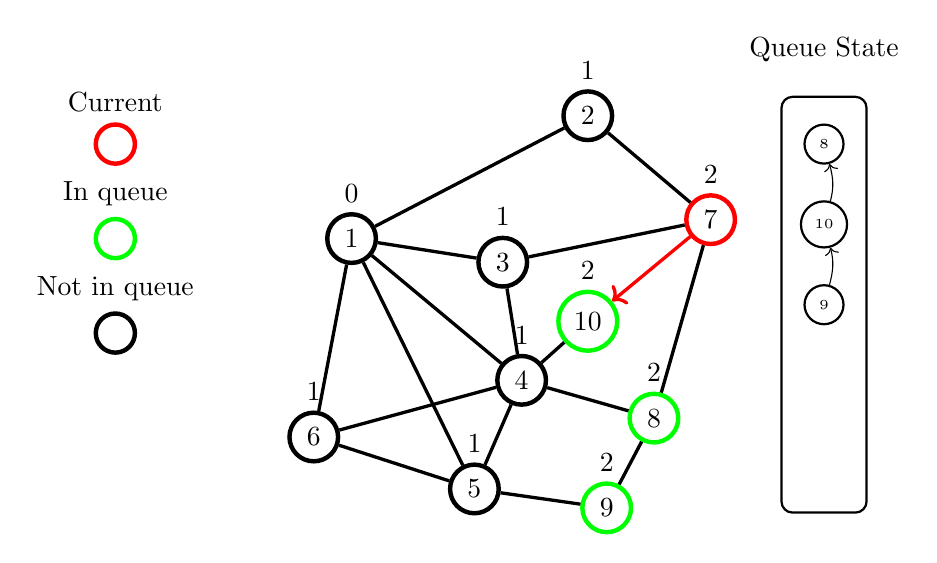
\begin{tikzpicture}[scale=1.2] 
\node[shape=circle, draw=red, 	ultra thick, scale=1.5pt, label={Current}] (U) at (-2.5, 1) {}; 
\node[shape=circle, draw=green,  ultra thick, scale=1.5pt, label={In queue}] (U) at (-2.5, 0) {}; 
\node[shape=circle, draw=black, ultra thick, scale=1.5pt, label={Not in queue}] (U) at (-2.5, -1) {}; 
\draw[thick, rounded corners,draw=black] (4.55, 1.5) rectangle ++(0.9, -1-4*0.85 );
\node[draw=white] at (5, 2) {Queue State} ; 
\node[shape=circle, draw=black, thick, minimum size=2pt] (U0) at (5, 1.0) {\tiny{8}}; 
\node[shape=circle, draw=black, thick, minimum size=2pt] (U1) at (5, 0.15000000000000002) {\tiny{10}}; 
\node[shape=circle, draw=black, thick, minimum size=2pt] (U2) at (5, -0.7) {\tiny{9}}; 
\path[->] (U1) edge [out=75, in=-75] (U0);
\path[->] (U2) edge [out=75, in=-75] (U1);
\node[shape=circle,draw=black, ultra thick, label={$0$}] (1) at (0,0) {1}; 
\node[shape=circle,draw=black, ultra thick, label={$1$}] (2) at (2.5,1.3) {2}; 
\node[shape=circle,draw=black, ultra thick, label={$1$}] (3) at (1.6,-0.25) {3}; 
\node[shape=circle,draw=black, ultra thick, label={$1$}] (4) at (1.8,-1.5) {4}; 
\node[shape=circle,draw=black, ultra thick, label={$1$}] (5) at (1.3,-2.65) {5}; 
\node[shape=circle,draw=black, ultra thick, label={$1$}] (6) at (-0.4,-2.1) {6}; 
\node[shape=circle,draw=red, ultra thick, label={$2$}] (7) at (3.8,0.2) {7}; 
\node[shape=circle,draw=green, ultra thick, label={$2$}] (8) at (3.2,-1.9) {8}; 
\node[shape=circle,draw=green, ultra thick, label={$2$}] (9) at (2.7,-2.85) {9}; 
\node[shape=circle,draw=green, ultra thick, label={$2$}] (10) at (2.5,-0.875) {10}; 
\path [-,very thick, draw=black] (1) edge  (2);
\path [-,very thick, draw=black] (1) edge  (3);
\path [-,very thick, draw=black] (1) edge  (4);
\path [-,very thick, draw=black] (1) edge  (5);
\path [-,very thick, draw=black] (1) edge  (6);
\path [-,very thick, draw=black] (2) edge  (7);
\path [-,very thick, draw=black] (3) edge  (7);
\path [-,very thick, draw=black] (3) edge  (4);
\path [-,very thick, draw=black] (4) edge  (5);
\path [-,very thick, draw=black] (4) edge  (6);
\path [-,very thick, draw=black] (4) edge  (8);
\path [-,very thick, draw=black] (4) edge  (10);
\path [-,very thick, draw=black] (5) edge  (6);
\path [-,very thick, draw=black] (5) edge  (9);
\path [-,very thick, draw=black] (7) edge  (8);
\path [->,very thick, draw=red] (7) edge  (10);
\path [-,very thick, draw=black] (8) edge  (9);
\end{tikzpicture} 
\end{figure} 
\end{frame} 
\begin{frame}{BFS : Example}
\begin{figure}
\vspace*{-1cm} 
\center
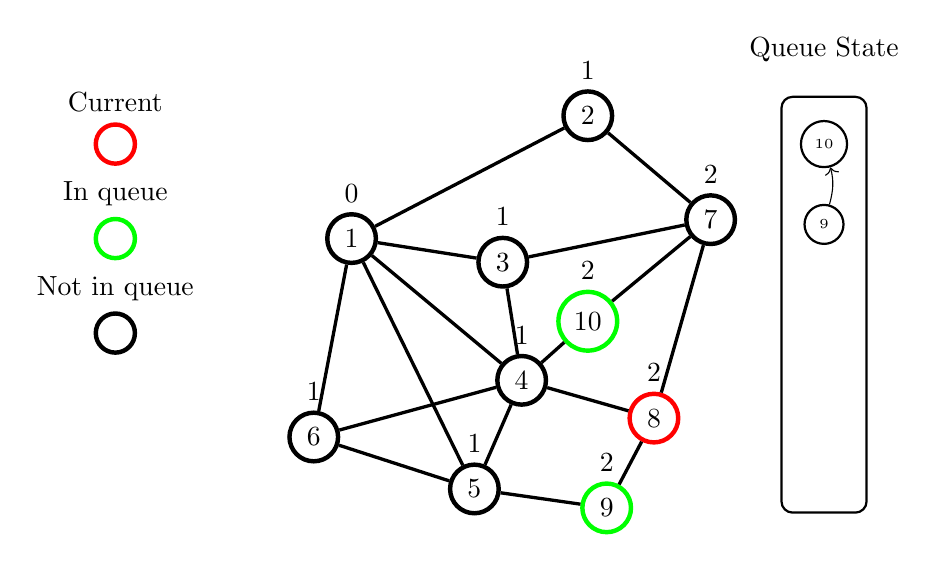
\begin{tikzpicture}[scale=1.2] 
\node[shape=circle, draw=red, 	ultra thick, scale=1.5pt, label={Current}] (U) at (-2.5, 1) {}; 
\node[shape=circle, draw=green,  ultra thick, scale=1.5pt, label={In queue}] (U) at (-2.5, 0) {}; 
\node[shape=circle, draw=black, ultra thick, scale=1.5pt, label={Not in queue}] (U) at (-2.5, -1) {}; 
\draw[thick, rounded corners,draw=black] (4.55, 1.5) rectangle ++(0.9, -1-4*0.85 );
\node[draw=white] at (5, 2) {Queue State} ; 
\node[shape=circle, draw=black, thick, minimum size=2pt] (U0) at (5, 1.0) {\tiny{10}}; 
\node[shape=circle, draw=black, thick, minimum size=2pt] (U1) at (5, 0.15000000000000002) {\tiny{9}}; 
\path[->] (U1) edge [out=75, in=-75] (U0);
\node[shape=circle,draw=black, ultra thick, label={$0$}] (1) at (0,0) {1}; 
\node[shape=circle,draw=black, ultra thick, label={$1$}] (2) at (2.5,1.3) {2}; 
\node[shape=circle,draw=black, ultra thick, label={$1$}] (3) at (1.6,-0.25) {3}; 
\node[shape=circle,draw=black, ultra thick, label={$1$}] (4) at (1.8,-1.5) {4}; 
\node[shape=circle,draw=black, ultra thick, label={$1$}] (5) at (1.3,-2.65) {5}; 
\node[shape=circle,draw=black, ultra thick, label={$1$}] (6) at (-0.4,-2.1) {6}; 
\node[shape=circle,draw=black, ultra thick, label={$2$}] (7) at (3.8,0.2) {7}; 
\node[shape=circle,draw=red, ultra thick, label={$2$}] (8) at (3.2,-1.9) {8}; 
\node[shape=circle,draw=green, ultra thick, label={$2$}] (9) at (2.7,-2.85) {9}; 
\node[shape=circle,draw=green, ultra thick, label={$2$}] (10) at (2.5,-0.875) {10}; 
\path [-,very thick, draw=black] (1) edge  (2);
\path [-,very thick, draw=black] (1) edge  (3);
\path [-,very thick, draw=black] (1) edge  (4);
\path [-,very thick, draw=black] (1) edge  (5);
\path [-,very thick, draw=black] (1) edge  (6);
\path [-,very thick, draw=black] (2) edge  (7);
\path [-,very thick, draw=black] (3) edge  (7);
\path [-,very thick, draw=black] (3) edge  (4);
\path [-,very thick, draw=black] (4) edge  (5);
\path [-,very thick, draw=black] (4) edge  (6);
\path [-,very thick, draw=black] (4) edge  (8);
\path [-,very thick, draw=black] (4) edge  (10);
\path [-,very thick, draw=black] (5) edge  (6);
\path [-,very thick, draw=black] (5) edge  (9);
\path [-,very thick, draw=black] (7) edge  (8);
\path [-,very thick, draw=black] (7) edge  (10);
\path [-,very thick, draw=black] (8) edge  (9);
\end{tikzpicture} 
\end{figure} 
\end{frame} 
\begin{frame}{BFS : Example}
\begin{figure}
\vspace*{-1cm} 
\center
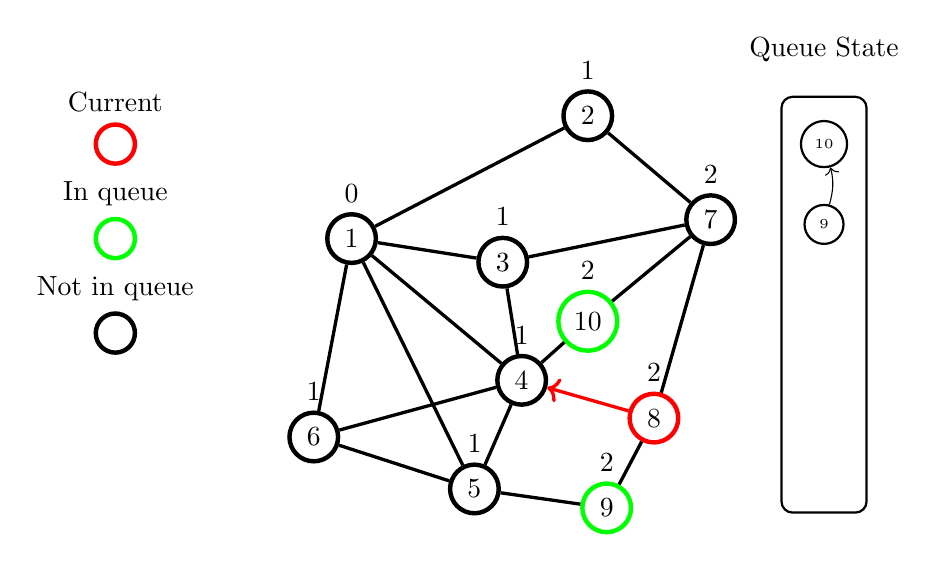
\begin{tikzpicture}[scale=1.2] 
\node[shape=circle, draw=red, 	ultra thick, scale=1.5pt, label={Current}] (U) at (-2.5, 1) {}; 
\node[shape=circle, draw=green,  ultra thick, scale=1.5pt, label={In queue}] (U) at (-2.5, 0) {}; 
\node[shape=circle, draw=black, ultra thick, scale=1.5pt, label={Not in queue}] (U) at (-2.5, -1) {}; 
\draw[thick, rounded corners,draw=black] (4.55, 1.5) rectangle ++(0.9, -1-4*0.85 );
\node[draw=white] at (5, 2) {Queue State} ; 
\node[shape=circle, draw=black, thick, minimum size=2pt] (U0) at (5, 1.0) {\tiny{10}}; 
\node[shape=circle, draw=black, thick, minimum size=2pt] (U1) at (5, 0.15000000000000002) {\tiny{9}}; 
\path[->] (U1) edge [out=75, in=-75] (U0);
\node[shape=circle,draw=black, ultra thick, label={$0$}] (1) at (0,0) {1}; 
\node[shape=circle,draw=black, ultra thick, label={$1$}] (2) at (2.5,1.3) {2}; 
\node[shape=circle,draw=black, ultra thick, label={$1$}] (3) at (1.6,-0.25) {3}; 
\node[shape=circle,draw=black, ultra thick, label={$1$}] (4) at (1.8,-1.5) {4}; 
\node[shape=circle,draw=black, ultra thick, label={$1$}] (5) at (1.3,-2.65) {5}; 
\node[shape=circle,draw=black, ultra thick, label={$1$}] (6) at (-0.4,-2.1) {6}; 
\node[shape=circle,draw=black, ultra thick, label={$2$}] (7) at (3.8,0.2) {7}; 
\node[shape=circle,draw=red, ultra thick, label={$2$}] (8) at (3.2,-1.9) {8}; 
\node[shape=circle,draw=green, ultra thick, label={$2$}] (9) at (2.7,-2.85) {9}; 
\node[shape=circle,draw=green, ultra thick, label={$2$}] (10) at (2.5,-0.875) {10}; 
\path [-,very thick, draw=black] (1) edge  (2);
\path [-,very thick, draw=black] (1) edge  (3);
\path [-,very thick, draw=black] (1) edge  (4);
\path [-,very thick, draw=black] (1) edge  (5);
\path [-,very thick, draw=black] (1) edge  (6);
\path [-,very thick, draw=black] (2) edge  (7);
\path [-,very thick, draw=black] (3) edge  (7);
\path [-,very thick, draw=black] (3) edge  (4);
\path [-,very thick, draw=black] (4) edge  (5);
\path [-,very thick, draw=black] (4) edge  (6);
\path [->,very thick, draw=red] (8) edge  (4);
\path [-,very thick, draw=black] (4) edge  (10);
\path [-,very thick, draw=black] (5) edge  (6);
\path [-,very thick, draw=black] (5) edge  (9);
\path [-,very thick, draw=black] (7) edge  (8);
\path [-,very thick, draw=black] (7) edge  (10);
\path [-,very thick, draw=black] (8) edge  (9);
\end{tikzpicture} 
\end{figure} 
\end{frame} 
\begin{frame}{BFS : Example}
\begin{figure}
\vspace*{-1cm} 
\center
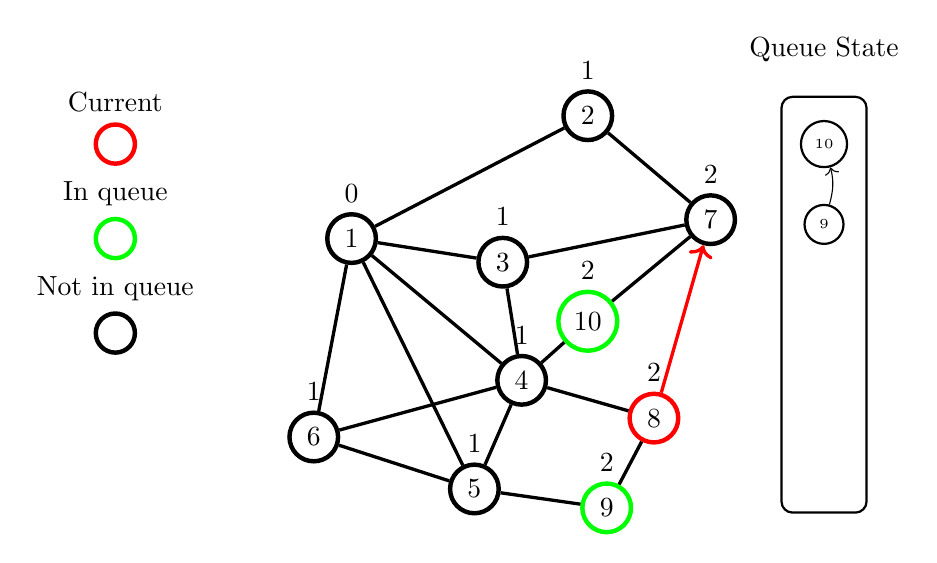
\begin{tikzpicture}[scale=1.2] 
\node[shape=circle, draw=red, 	ultra thick, scale=1.5pt, label={Current}] (U) at (-2.5, 1) {}; 
\node[shape=circle, draw=green,  ultra thick, scale=1.5pt, label={In queue}] (U) at (-2.5, 0) {}; 
\node[shape=circle, draw=black, ultra thick, scale=1.5pt, label={Not in queue}] (U) at (-2.5, -1) {}; 
\draw[thick, rounded corners,draw=black] (4.55, 1.5) rectangle ++(0.9, -1-4*0.85 );
\node[draw=white] at (5, 2) {Queue State} ; 
\node[shape=circle, draw=black, thick, minimum size=2pt] (U0) at (5, 1.0) {\tiny{10}}; 
\node[shape=circle, draw=black, thick, minimum size=2pt] (U1) at (5, 0.15000000000000002) {\tiny{9}}; 
\path[->] (U1) edge [out=75, in=-75] (U0);
\node[shape=circle,draw=black, ultra thick, label={$0$}] (1) at (0,0) {1}; 
\node[shape=circle,draw=black, ultra thick, label={$1$}] (2) at (2.5,1.3) {2}; 
\node[shape=circle,draw=black, ultra thick, label={$1$}] (3) at (1.6,-0.25) {3}; 
\node[shape=circle,draw=black, ultra thick, label={$1$}] (4) at (1.8,-1.5) {4}; 
\node[shape=circle,draw=black, ultra thick, label={$1$}] (5) at (1.3,-2.65) {5}; 
\node[shape=circle,draw=black, ultra thick, label={$1$}] (6) at (-0.4,-2.1) {6}; 
\node[shape=circle,draw=black, ultra thick, label={$2$}] (7) at (3.8,0.2) {7}; 
\node[shape=circle,draw=red, ultra thick, label={$2$}] (8) at (3.2,-1.9) {8}; 
\node[shape=circle,draw=green, ultra thick, label={$2$}] (9) at (2.7,-2.85) {9}; 
\node[shape=circle,draw=green, ultra thick, label={$2$}] (10) at (2.5,-0.875) {10}; 
\path [-,very thick, draw=black] (1) edge  (2);
\path [-,very thick, draw=black] (1) edge  (3);
\path [-,very thick, draw=black] (1) edge  (4);
\path [-,very thick, draw=black] (1) edge  (5);
\path [-,very thick, draw=black] (1) edge  (6);
\path [-,very thick, draw=black] (2) edge  (7);
\path [-,very thick, draw=black] (3) edge  (7);
\path [-,very thick, draw=black] (3) edge  (4);
\path [-,very thick, draw=black] (4) edge  (5);
\path [-,very thick, draw=black] (4) edge  (6);
\path [-,very thick, draw=black] (4) edge  (8);
\path [-,very thick, draw=black] (4) edge  (10);
\path [-,very thick, draw=black] (5) edge  (6);
\path [-,very thick, draw=black] (5) edge  (9);
\path [->,very thick, draw=red] (8) edge  (7);
\path [-,very thick, draw=black] (7) edge  (10);
\path [-,very thick, draw=black] (8) edge  (9);
\end{tikzpicture} 
\end{figure} 
\end{frame} 
\begin{frame}{BFS : Example}
\begin{figure}
\vspace*{-1cm} 
\center
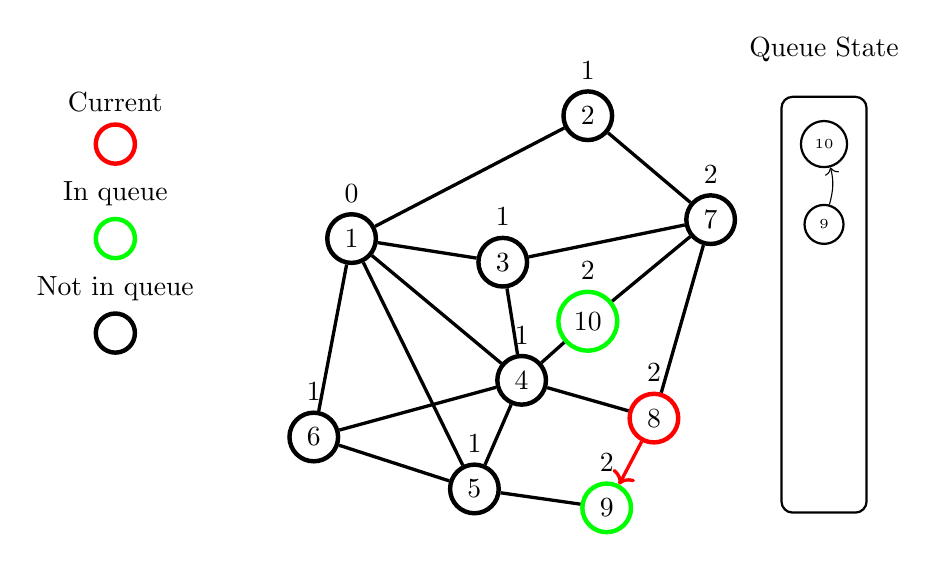
\begin{tikzpicture}[scale=1.2] 
\node[shape=circle, draw=red, 	ultra thick, scale=1.5pt, label={Current}] (U) at (-2.5, 1) {}; 
\node[shape=circle, draw=green,  ultra thick, scale=1.5pt, label={In queue}] (U) at (-2.5, 0) {}; 
\node[shape=circle, draw=black, ultra thick, scale=1.5pt, label={Not in queue}] (U) at (-2.5, -1) {}; 
\draw[thick, rounded corners,draw=black] (4.55, 1.5) rectangle ++(0.9, -1-4*0.85 );
\node[draw=white] at (5, 2) {Queue State} ; 
\node[shape=circle, draw=black, thick, minimum size=2pt] (U0) at (5, 1.0) {\tiny{10}}; 
\node[shape=circle, draw=black, thick, minimum size=2pt] (U1) at (5, 0.15000000000000002) {\tiny{9}}; 
\path[->] (U1) edge [out=75, in=-75] (U0);
\node[shape=circle,draw=black, ultra thick, label={$0$}] (1) at (0,0) {1}; 
\node[shape=circle,draw=black, ultra thick, label={$1$}] (2) at (2.5,1.3) {2}; 
\node[shape=circle,draw=black, ultra thick, label={$1$}] (3) at (1.6,-0.25) {3}; 
\node[shape=circle,draw=black, ultra thick, label={$1$}] (4) at (1.8,-1.5) {4}; 
\node[shape=circle,draw=black, ultra thick, label={$1$}] (5) at (1.3,-2.65) {5}; 
\node[shape=circle,draw=black, ultra thick, label={$1$}] (6) at (-0.4,-2.1) {6}; 
\node[shape=circle,draw=black, ultra thick, label={$2$}] (7) at (3.8,0.2) {7}; 
\node[shape=circle,draw=red, ultra thick, label={$2$}] (8) at (3.2,-1.9) {8}; 
\node[shape=circle,draw=green, ultra thick, label={$2$}] (9) at (2.7,-2.85) {9}; 
\node[shape=circle,draw=green, ultra thick, label={$2$}] (10) at (2.5,-0.875) {10}; 
\path [-,very thick, draw=black] (1) edge  (2);
\path [-,very thick, draw=black] (1) edge  (3);
\path [-,very thick, draw=black] (1) edge  (4);
\path [-,very thick, draw=black] (1) edge  (5);
\path [-,very thick, draw=black] (1) edge  (6);
\path [-,very thick, draw=black] (2) edge  (7);
\path [-,very thick, draw=black] (3) edge  (7);
\path [-,very thick, draw=black] (3) edge  (4);
\path [-,very thick, draw=black] (4) edge  (5);
\path [-,very thick, draw=black] (4) edge  (6);
\path [-,very thick, draw=black] (4) edge  (8);
\path [-,very thick, draw=black] (4) edge  (10);
\path [-,very thick, draw=black] (5) edge  (6);
\path [-,very thick, draw=black] (5) edge  (9);
\path [-,very thick, draw=black] (7) edge  (8);
\path [-,very thick, draw=black] (7) edge  (10);
\path [->,very thick, draw=red] (8) edge  (9);
\end{tikzpicture} 
\end{figure} 
\end{frame} 
\begin{frame}{BFS : Example}
\begin{figure}
\vspace*{-1cm} 
\center
\begin{tikzpicture}[scale=1.2] 
\node[shape=circle, draw=red, 	ultra thick, scale=1.5pt, label={Current}] (U) at (-2.5, 1) {}; 
\node[shape=circle, draw=green,  ultra thick, scale=1.5pt, label={In queue}] (U) at (-2.5, 0) {}; 
\node[shape=circle, draw=black, ultra thick, scale=1.5pt, label={Not in queue}] (U) at (-2.5, -1) {}; 
\draw[thick, rounded corners,draw=black] (4.55, 1.5) rectangle ++(0.9, -1-4*0.85 );
\node[draw=white] at (5, 2) {Queue State} ; 
\node[shape=circle, draw=black, thick, minimum size=2pt] (U0) at (5, 1.0) {\tiny{9}}; 
\node[shape=circle,draw=black, ultra thick, label={$0$}] (1) at (0,0) {1}; 
\node[shape=circle,draw=black, ultra thick, label={$1$}] (2) at (2.5,1.3) {2}; 
\node[shape=circle,draw=black, ultra thick, label={$1$}] (3) at (1.6,-0.25) {3}; 
\node[shape=circle,draw=black, ultra thick, label={$1$}] (4) at (1.8,-1.5) {4}; 
\node[shape=circle,draw=black, ultra thick, label={$1$}] (5) at (1.3,-2.65) {5}; 
\node[shape=circle,draw=black, ultra thick, label={$1$}] (6) at (-0.4,-2.1) {6}; 
\node[shape=circle,draw=black, ultra thick, label={$2$}] (7) at (3.8,0.2) {7}; 
\node[shape=circle,draw=black, ultra thick, label={$2$}] (8) at (3.2,-1.9) {8}; 
\node[shape=circle,draw=green, ultra thick, label={$2$}] (9) at (2.7,-2.85) {9}; 
\node[shape=circle,draw=red, ultra thick, label={$2$}] (10) at (2.5,-0.875) {10}; 
\path [-,very thick, draw=black] (1) edge  (2);
\path [-,very thick, draw=black] (1) edge  (3);
\path [-,very thick, draw=black] (1) edge  (4);
\path [-,very thick, draw=black] (1) edge  (5);
\path [-,very thick, draw=black] (1) edge  (6);
\path [-,very thick, draw=black] (2) edge  (7);
\path [-,very thick, draw=black] (3) edge  (7);
\path [-,very thick, draw=black] (3) edge  (4);
\path [-,very thick, draw=black] (4) edge  (5);
\path [-,very thick, draw=black] (4) edge  (6);
\path [-,very thick, draw=black] (4) edge  (8);
\path [-,very thick, draw=black] (4) edge  (10);
\path [-,very thick, draw=black] (5) edge  (6);
\path [-,very thick, draw=black] (5) edge  (9);
\path [-,very thick, draw=black] (7) edge  (8);
\path [-,very thick, draw=black] (7) edge  (10);
\path [-,very thick, draw=black] (8) edge  (9);
\end{tikzpicture} 
\end{figure} 
\end{frame} 
\begin{frame}{BFS : Example}
\begin{figure}
\vspace*{-1cm} 
\center
\begin{tikzpicture}[scale=1.2] 
\node[shape=circle, draw=red, 	ultra thick, scale=1.5pt, label={Current}] (U) at (-2.5, 1) {}; 
\node[shape=circle, draw=green,  ultra thick, scale=1.5pt, label={In queue}] (U) at (-2.5, 0) {}; 
\node[shape=circle, draw=black, ultra thick, scale=1.5pt, label={Not in queue}] (U) at (-2.5, -1) {}; 
\draw[thick, rounded corners,draw=black] (4.55, 1.5) rectangle ++(0.9, -1-4*0.85 );
\node[draw=white] at (5, 2) {Queue State} ; 
\node[shape=circle, draw=black, thick, minimum size=2pt] (U0) at (5, 1.0) {\tiny{9}}; 
\node[shape=circle,draw=black, ultra thick, label={$0$}] (1) at (0,0) {1}; 
\node[shape=circle,draw=black, ultra thick, label={$1$}] (2) at (2.5,1.3) {2}; 
\node[shape=circle,draw=black, ultra thick, label={$1$}] (3) at (1.6,-0.25) {3}; 
\node[shape=circle,draw=black, ultra thick, label={$1$}] (4) at (1.8,-1.5) {4}; 
\node[shape=circle,draw=black, ultra thick, label={$1$}] (5) at (1.3,-2.65) {5}; 
\node[shape=circle,draw=black, ultra thick, label={$1$}] (6) at (-0.4,-2.1) {6}; 
\node[shape=circle,draw=black, ultra thick, label={$2$}] (7) at (3.8,0.2) {7}; 
\node[shape=circle,draw=black, ultra thick, label={$2$}] (8) at (3.2,-1.9) {8}; 
\node[shape=circle,draw=green, ultra thick, label={$2$}] (9) at (2.7,-2.85) {9}; 
\node[shape=circle,draw=red, ultra thick, label={$2$}] (10) at (2.5,-0.875) {10}; 
\path [-,very thick, draw=black] (1) edge  (2);
\path [-,very thick, draw=black] (1) edge  (3);
\path [-,very thick, draw=black] (1) edge  (4);
\path [-,very thick, draw=black] (1) edge  (5);
\path [-,very thick, draw=black] (1) edge  (6);
\path [-,very thick, draw=black] (2) edge  (7);
\path [-,very thick, draw=black] (3) edge  (7);
\path [-,very thick, draw=black] (3) edge  (4);
\path [-,very thick, draw=black] (4) edge  (5);
\path [-,very thick, draw=black] (4) edge  (6);
\path [-,very thick, draw=black] (4) edge  (8);
\path [->,very thick, draw=red] (10) edge  (4);
\path [-,very thick, draw=black] (5) edge  (6);
\path [-,very thick, draw=black] (5) edge  (9);
\path [-,very thick, draw=black] (7) edge  (8);
\path [-,very thick, draw=black] (7) edge  (10);
\path [-,very thick, draw=black] (8) edge  (9);
\end{tikzpicture} 
\end{figure} 
\end{frame} 
\begin{frame}{BFS : Example}
\begin{figure}
\vspace*{-1cm} 
\center
\begin{tikzpicture}[scale=1.2] 
\node[shape=circle, draw=red, 	ultra thick, scale=1.5pt, label={Current}] (U) at (-2.5, 1) {}; 
\node[shape=circle, draw=green,  ultra thick, scale=1.5pt, label={In queue}] (U) at (-2.5, 0) {}; 
\node[shape=circle, draw=black, ultra thick, scale=1.5pt, label={Not in queue}] (U) at (-2.5, -1) {}; 
\draw[thick, rounded corners,draw=black] (4.55, 1.5) rectangle ++(0.9, -1-4*0.85 );
\node[draw=white] at (5, 2) {Queue State} ; 
\node[shape=circle, draw=black, thick, minimum size=2pt] (U0) at (5, 1.0) {\tiny{9}}; 
\node[shape=circle,draw=black, ultra thick, label={$0$}] (1) at (0,0) {1}; 
\node[shape=circle,draw=black, ultra thick, label={$1$}] (2) at (2.5,1.3) {2}; 
\node[shape=circle,draw=black, ultra thick, label={$1$}] (3) at (1.6,-0.25) {3}; 
\node[shape=circle,draw=black, ultra thick, label={$1$}] (4) at (1.8,-1.5) {4}; 
\node[shape=circle,draw=black, ultra thick, label={$1$}] (5) at (1.3,-2.65) {5}; 
\node[shape=circle,draw=black, ultra thick, label={$1$}] (6) at (-0.4,-2.1) {6}; 
\node[shape=circle,draw=black, ultra thick, label={$2$}] (7) at (3.8,0.2) {7}; 
\node[shape=circle,draw=black, ultra thick, label={$2$}] (8) at (3.2,-1.9) {8}; 
\node[shape=circle,draw=green, ultra thick, label={$2$}] (9) at (2.7,-2.85) {9}; 
\node[shape=circle,draw=red, ultra thick, label={$2$}] (10) at (2.5,-0.875) {10}; 
\path [-,very thick, draw=black] (1) edge  (2);
\path [-,very thick, draw=black] (1) edge  (3);
\path [-,very thick, draw=black] (1) edge  (4);
\path [-,very thick, draw=black] (1) edge  (5);
\path [-,very thick, draw=black] (1) edge  (6);
\path [-,very thick, draw=black] (2) edge  (7);
\path [-,very thick, draw=black] (3) edge  (7);
\path [-,very thick, draw=black] (3) edge  (4);
\path [-,very thick, draw=black] (4) edge  (5);
\path [-,very thick, draw=black] (4) edge  (6);
\path [-,very thick, draw=black] (4) edge  (8);
\path [-,very thick, draw=black] (4) edge  (10);
\path [-,very thick, draw=black] (5) edge  (6);
\path [-,very thick, draw=black] (5) edge  (9);
\path [-,very thick, draw=black] (7) edge  (8);
\path [->,very thick, draw=red] (10) edge  (7);
\path [-,very thick, draw=black] (8) edge  (9);
\end{tikzpicture} 
\end{figure} 
\end{frame} 
\begin{frame}{BFS : Example}
\begin{figure}
\vspace*{-1cm} 
\center
\begin{tikzpicture}[scale=1.2] 
\node[shape=circle, draw=red, 	ultra thick, scale=1.5pt, label={Current}] (U) at (-2.5, 1) {}; 
\node[shape=circle, draw=green,  ultra thick, scale=1.5pt, label={In queue}] (U) at (-2.5, 0) {}; 
\node[shape=circle, draw=black, ultra thick, scale=1.5pt, label={Not in queue}] (U) at (-2.5, -1) {}; 
\draw[thick, rounded corners,draw=black] (4.55, 1.5) rectangle ++(0.9, -1-4*0.85 );
\node[draw=white] at (5, 2) {Queue State} ; 
\node[shape=circle,draw=black, ultra thick, label={$0$}] (1) at (0,0) {1}; 
\node[shape=circle,draw=black, ultra thick, label={$1$}] (2) at (2.5,1.3) {2}; 
\node[shape=circle,draw=black, ultra thick, label={$1$}] (3) at (1.6,-0.25) {3}; 
\node[shape=circle,draw=black, ultra thick, label={$1$}] (4) at (1.8,-1.5) {4}; 
\node[shape=circle,draw=black, ultra thick, label={$1$}] (5) at (1.3,-2.65) {5}; 
\node[shape=circle,draw=black, ultra thick, label={$1$}] (6) at (-0.4,-2.1) {6}; 
\node[shape=circle,draw=black, ultra thick, label={$2$}] (7) at (3.8,0.2) {7}; 
\node[shape=circle,draw=black, ultra thick, label={$2$}] (8) at (3.2,-1.9) {8}; 
\node[shape=circle,draw=red, ultra thick, label={$2$}] (9) at (2.7,-2.85) {9}; 
\node[shape=circle,draw=black, ultra thick, label={$2$}] (10) at (2.5,-0.875) {10}; 
\path [-,very thick, draw=black] (1) edge  (2);
\path [-,very thick, draw=black] (1) edge  (3);
\path [-,very thick, draw=black] (1) edge  (4);
\path [-,very thick, draw=black] (1) edge  (5);
\path [-,very thick, draw=black] (1) edge  (6);
\path [-,very thick, draw=black] (2) edge  (7);
\path [-,very thick, draw=black] (3) edge  (7);
\path [-,very thick, draw=black] (3) edge  (4);
\path [-,very thick, draw=black] (4) edge  (5);
\path [-,very thick, draw=black] (4) edge  (6);
\path [-,very thick, draw=black] (4) edge  (8);
\path [-,very thick, draw=black] (4) edge  (10);
\path [-,very thick, draw=black] (5) edge  (6);
\path [-,very thick, draw=black] (5) edge  (9);
\path [-,very thick, draw=black] (7) edge  (8);
\path [-,very thick, draw=black] (7) edge  (10);
\path [-,very thick, draw=black] (8) edge  (9);
\end{tikzpicture} 
\end{figure} 
\end{frame} 
\begin{frame}{BFS : Example}
\begin{figure}
\vspace*{-1cm} 
\center
\begin{tikzpicture}[scale=1.2] 
\node[shape=circle, draw=red, 	ultra thick, scale=1.5pt, label={Current}] (U) at (-2.5, 1) {}; 
\node[shape=circle, draw=green,  ultra thick, scale=1.5pt, label={In queue}] (U) at (-2.5, 0) {}; 
\node[shape=circle, draw=black, ultra thick, scale=1.5pt, label={Not in queue}] (U) at (-2.5, -1) {}; 
\draw[thick, rounded corners,draw=black] (4.55, 1.5) rectangle ++(0.9, -1-4*0.85 );
\node[draw=white] at (5, 2) {Queue State} ; 
\node[shape=circle,draw=black, ultra thick, label={$0$}] (1) at (0,0) {1}; 
\node[shape=circle,draw=black, ultra thick, label={$1$}] (2) at (2.5,1.3) {2}; 
\node[shape=circle,draw=black, ultra thick, label={$1$}] (3) at (1.6,-0.25) {3}; 
\node[shape=circle,draw=black, ultra thick, label={$1$}] (4) at (1.8,-1.5) {4}; 
\node[shape=circle,draw=black, ultra thick, label={$1$}] (5) at (1.3,-2.65) {5}; 
\node[shape=circle,draw=black, ultra thick, label={$1$}] (6) at (-0.4,-2.1) {6}; 
\node[shape=circle,draw=black, ultra thick, label={$2$}] (7) at (3.8,0.2) {7}; 
\node[shape=circle,draw=black, ultra thick, label={$2$}] (8) at (3.2,-1.9) {8}; 
\node[shape=circle,draw=red, ultra thick, label={$2$}] (9) at (2.7,-2.85) {9}; 
\node[shape=circle,draw=black, ultra thick, label={$2$}] (10) at (2.5,-0.875) {10}; 
\path [-,very thick, draw=black] (1) edge  (2);
\path [-,very thick, draw=black] (1) edge  (3);
\path [-,very thick, draw=black] (1) edge  (4);
\path [-,very thick, draw=black] (1) edge  (5);
\path [-,very thick, draw=black] (1) edge  (6);
\path [-,very thick, draw=black] (2) edge  (7);
\path [-,very thick, draw=black] (3) edge  (7);
\path [-,very thick, draw=black] (3) edge  (4);
\path [-,very thick, draw=black] (4) edge  (5);
\path [-,very thick, draw=black] (4) edge  (6);
\path [-,very thick, draw=black] (4) edge  (8);
\path [-,very thick, draw=black] (4) edge  (10);
\path [-,very thick, draw=black] (5) edge  (6);
\path [->,very thick, draw=red] (9) edge  (5);
\path [-,very thick, draw=black] (7) edge  (8);
\path [-,very thick, draw=black] (7) edge  (10);
\path [-,very thick, draw=black] (8) edge  (9);
\end{tikzpicture} 
\end{figure} 
\end{frame} 
\begin{frame}{BFS : Example}
\begin{figure}
\vspace*{-1cm} 
\center
\begin{tikzpicture}[scale=1.2] 
\node[shape=circle, draw=red, 	ultra thick, scale=1.5pt, label={Current}] (U) at (-2.5, 1) {}; 
\node[shape=circle, draw=green,  ultra thick, scale=1.5pt, label={In queue}] (U) at (-2.5, 0) {}; 
\node[shape=circle, draw=black, ultra thick, scale=1.5pt, label={Not in queue}] (U) at (-2.5, -1) {}; 
\draw[thick, rounded corners,draw=black] (4.55, 1.5) rectangle ++(0.9, -1-4*0.85 );
\node[draw=white] at (5, 2) {Queue State} ; 
\node[shape=circle,draw=black, ultra thick, label={$0$}] (1) at (0,0) {1}; 
\node[shape=circle,draw=black, ultra thick, label={$1$}] (2) at (2.5,1.3) {2}; 
\node[shape=circle,draw=black, ultra thick, label={$1$}] (3) at (1.6,-0.25) {3}; 
\node[shape=circle,draw=black, ultra thick, label={$1$}] (4) at (1.8,-1.5) {4}; 
\node[shape=circle,draw=black, ultra thick, label={$1$}] (5) at (1.3,-2.65) {5}; 
\node[shape=circle,draw=black, ultra thick, label={$1$}] (6) at (-0.4,-2.1) {6}; 
\node[shape=circle,draw=black, ultra thick, label={$2$}] (7) at (3.8,0.2) {7}; 
\node[shape=circle,draw=black, ultra thick, label={$2$}] (8) at (3.2,-1.9) {8}; 
\node[shape=circle,draw=red, ultra thick, label={$2$}] (9) at (2.7,-2.85) {9}; 
\node[shape=circle,draw=black, ultra thick, label={$2$}] (10) at (2.5,-0.875) {10}; 
\path [-,very thick, draw=black] (1) edge  (2);
\path [-,very thick, draw=black] (1) edge  (3);
\path [-,very thick, draw=black] (1) edge  (4);
\path [-,very thick, draw=black] (1) edge  (5);
\path [-,very thick, draw=black] (1) edge  (6);
\path [-,very thick, draw=black] (2) edge  (7);
\path [-,very thick, draw=black] (3) edge  (7);
\path [-,very thick, draw=black] (3) edge  (4);
\path [-,very thick, draw=black] (4) edge  (5);
\path [-,very thick, draw=black] (4) edge  (6);
\path [-,very thick, draw=black] (4) edge  (8);
\path [-,very thick, draw=black] (4) edge  (10);
\path [-,very thick, draw=black] (5) edge  (6);
\path [-,very thick, draw=black] (5) edge  (9);
\path [-,very thick, draw=black] (7) edge  (8);
\path [-,very thick, draw=black] (7) edge  (10);
\path [->,very thick, draw=red] (9) edge  (8);
\end{tikzpicture} 
\end{figure} 
\end{frame} 



\end{document}
